
%NDSS
%\documentclass[conference]{IEEEtran}
%\pagestyle{plain}
%CHES
%CHES
\documentclass[submission]{iacrtrans}

\newif\ifdraft
%\drafttrue
%\usepackage{appendix}
\usepackage{graphicx}
%\usepackage{adjustbox}
%\usepackage{enumitem}
%\usepackage[small]{caption} 
\usepackage{amsmath,amsthm,amssymb}
\usepackage{mathtools}
\usepackage{mathrsfs}
\usepackage{xspace}
\usepackage{url}
%\usepackage{subfig}
%\usepackage[compact]{titlesec}
%\usepackage{tikz}
%\usepackage{float}
%\usepackage{subfig}
\usepackage{listings}
\usepackage[ruled,linesnumbered,vlined]{algorithm2e}
\usepackage{rotating}
\usepackage{longtable}
\usepackage{balance}
%\usepackage{mathtools}
%\usepackage{array}
%\usepackage{booktabs}
\usepackage{multirow, bigdelim}
\usepackage{cite}
\usepackage{hyphenat}
\usepackage{adjustbox}
%\usepackage[graphicx]{realboxes}
%\usepackage{rotating}

%% Compacting 
%%
%\usepackage[
%all=normal,floats=tight
%,paragraphs=tight
%,wordspacing=tight
%,mathspacing=tight
%,mathdisplays=tight
%]{savetrees}
%\usepackage[compact]{titlesec}


\lstset{
  basicstyle=\ttfamily,
  %numbers=left,
  %numberstyle=\tiny,
  columns=fullflexible,
  showstringspaces=false,
  commentstyle=\color{gray}\upshape
}

\lstdefinelanguage{XML}
{
  morestring=[b]",
  morestring=[s]{>}{<},
  morecomment=[s]{<?}{?>},
  stringstyle=\color{black},
  basicstyle={\scriptsize\ttfamily\bfseries\color{black}},
  identifierstyle=\color{darkblue},
  keywordstyle=\color{blue},
  morekeywords={RegEx,Tag,Type,Input}
}
\renewcommand\lstlistingname{Specification}

\usepackage{color}
\definecolor{gray}{rgb}{0.4,0.4,0.4}
\definecolor{darkblue}{rgb}{0.0,0.0,0.6}
\definecolor{cyan}{rgb}{0.0,0.6,0.6}

\newcommand{\red}[1]{\textcolor{red}{#1}} 

\newcommand{\dy}[1]{\textcolor{blue}{DY: #1}} 
\newcommand{\ad}[1]{\textcolor{red}{Aritra: #1}}
\newcommand{\srdjan}[1]{\textcolor{brown}{Srdjan: #1}}
\newcommand{\todo}[1]{\textcolor{red}{TODO: #1}}
\newcommand{\tocite}{\textcolor{blue}{[cite]}}
\newcommand{\blue}[1]{\textcolor{blue}{#1}}

%\widowpenalty 200000
%\clubpenalty 200000
%\usepackage[compact]{titlesec}

\newcommand{\name}{\textsc{IntegriKey}\xspace}
\newcommand{\tool}{\textsc{IntegriTool}\xspace}
%\newcommand{\tool}{\name}
\newcommand{\device}{\textsc{Bridge}\xspace}
\newcommand{\server}{\textsc{Server}\xspace}

\newcommand{\toolname}{\name\xspace}
\newcommand{\credential}{$\mathcal{C}_S$\xspace}
\newcommand{\credentialServer}[1]{$\mathcal{C}_{#1}$\xspace}
\newcommand{\serverside}{\name tool\xspace}

\newcommand{\usb}{USB\xspace}
\newcommand{\bluetooth}{Bluetooth\xspace}
\newcommand{\webusb}{WebUSB\xspace}
\newcommand{\html}{HTML\xspace}
\newcommand{\webbt}{WebBluetooth\xspace}
\newcommand{\sensitive}{$\mathcal{F}_s$\xspace}
\newcommand{\insensitive}{$\mathcal{F}_p$\xspace}
\newcommand{\redir}{$\mathcal{S}_{redir}$\xspace}
\newcommand{\http}{HTTP\xspace}
\newcommand{\https}{HTTPS\xspace}
\newcommand{\tls}{TLS\xspace}
\newcommand{\ssl}{\texttt{SSl}\xspace}
\newcommand{\onSelect}{\texttt{onSelect()}\xspace}

%\newcommand{\myparagraph}[1]{{\scshape \bfseries #1.}}
%\newcommand{\myparagraph}[1]{\noindent{\textbf{#1.}}}
\newcommand{\myparagraph}[1]{\paragraph{#1.}}

\newcommand{\webrtc}{\texttt{WebRTC}\xspace}
\newcommand{\js}{JavaScript\xspace}
\newcommand{\relay}{$\mathcal{S}_{relay}$\xspace}
\newcommand{\messenger}{$\mathcal{S}_{messenger}$\xspace}
\newcommand{\serial}{\texttt{serial}\xspace}
\newcommand{\String}{\texttt{string}\xspace}
\newcommand{\integer}{\texttt{integer}\xspace}
\newcommand{\float}{\texttt{float}\xspace}
\newcommand{\menu}{\texttt{menu}\xspace}
\newcommand{\radio}{\texttt{radio button}\xspace}
\newcommand{\Boolean}{\texttt{boolean}\xspace}
\newcommand{\Date}{\texttt{date}\xspace}
\newcommand{\Menu}{\texttt{menu}\xspace}
\newcommand{\Time}{\texttt{time}\xspace}
\newcommand{\mytab}{~~~}
\newcommand{\java}{\textsc{Java}\xspace}

\definecolor{Gray}{gray}{0.85}
\definecolor{LightCyan}{rgb}{0.88,1,1}

\newcommand\MyLBrace[2]{%
  \left.\rule{0pt}{#1}\right\}\text{#2}}

%\newcounter{myExampleCounter}
%\setcounter{myExampleCounter}{-1} % Start with -1.
%\refstepcounter{myExampleCounter}


\newcounter{para}
\newcommand\mypara{\par\refstepcounter{para}\thepara.\space}
\newcommand{\myparapara}[1]{\mypara\textbf{{#1.}}\xspace}

%\newcommand{\redCircle}{$\otimes$}
%\newcommand{\greenCircle}[2][black,fill=white]{\tikz[baseline=-0.5ex]\draw[#1,radius=3pt]
%(0,0) circle ;}
%\newcommand{\yellowCircle}[2][black,fill=black]{\tikz[baseline=-0.5ex]\draw[#1,radius=3pt]
%(0,0) circle ;}

\DeclareGraphicsExtensions{.pdf,.jpeg,.png,.jpg}

%\hyphenation{Integri-Key}

% \newcommand{\redCircle}[][red,fill=red]{\tikz[baseline=-0.5ex]\draw[#1,radius=3pt]
% (0,0) circle ;}
% \newcommand{\greenCircle}[2][green,fill=green]{\tikz[baseline=-0.5ex]\draw[#1,radius=3pt]
% (0,0) circle ;}
% \newcommand{\yellowCircle}[2][red,fill=yellow]{\tikz[baseline=-0.5ex]\draw[#1,radius=3pt]
% (0,0) circle ;}

%------------------------------------------------------------------------------
%                                Space savers.
%------------------------------------------------------------------------------

% This mylist environment indents items, and saves less space than the above.
\newcounter{myctr}
\newenvironment{mylist}{\begin{list}{\arabic{myctr})}
{\usecounter{myctr}
\setlength{\topsep}{1mm}\setlength{\itemsep}{0.5mm}
\setlength{\parsep}{0.5mm}
\setlength{\itemindent}{0mm}\setlength{\partopsep}{0mm}
\setlength{\labelwidth}{-2mm}
\setlength{\leftmargin}{1mm}}}{\end{list}}

\newcounter{myctrA}
\newenvironment{mylistAlph}{\begin{list}{\textbf{\Alph{myctrA}})}
{\usecounter{myctrA}
\setlength{\topsep}{1mm}\setlength{\itemsep}{0.5mm}
\setlength{\parsep}{0.5mm}
\setlength{\itemindent}{0mm}\setlength{\partopsep}{0mm}
\setlength{\labelwidth}{-2mm}
\setlength{\leftmargin}{0.5mm}}}{\end{list}}

% Space saving List environment for itemizing.
\newenvironment{mybullet}{\begin{list}{$\bullet$}
{\setlength{\topsep}{1mm}\setlength{\itemsep}{0.5mm}
\setlength{\parsep}{0.5mm}
\setlength{\itemindent}{4mm}\setlength{\partopsep}{0mm}
\setlength{\labelwidth}{-2mm}
\setlength{\leftmargin}{2mm}}}{\end{list}}


\graphicspath{{figures/}}

\settopmatter{authorsperrow=4}

\title[\name]{\name: Hardened SGX Attestation by \\ Proximity Verification} 

\author{Aritra Dhar}
\affiliation{
\institution{ETH Zurich}
aritra.dhar@inf.ethz.ch
}
\author{Ivan Puddu}
\affiliation{
\institution{ETH Zurich}
ivan.puddu@inf.ethz.ch
}

\author{Kari Kostiainen}
\affiliation{
\institution{ETH Zurich}
kari.kostiainen@inf.ethz.ch
}
\author{Srdjan Capkun}
\affiliation{
\institution{ETH Zurich}
srdjan.capkun@inf.ethz.ch
}

%Ivan Puddu, Kari Kostiainen, Srdjan Capkun}
\copyrightyear{2020}
\acmYear{2020}
\setcopyright{acmcopyright}
\acmConference[CODASPY '20]{Proceedings of the Tenth ACM Conference on Data and
Application Security and Privacy}{March 16--18, 2020}{New Orleans, LA, USA}
\acmBooktitle{Proceedings of the Tenth ACM Conference on Data and Application Security and
Privacy (CODASPY '20), March 16--18, 2020, New Orleans, LA, USA}
\acmPrice{15.00}
\acmDOI{10.1145/3374664.3375726}
\acmISBN{978-1-4503-7107-0/20/03}

\begin{document}
\fancyhead{}

%\acmConference[Submission]{}{}

\begin{abstract}
Intel SGX enables protected enclaves on untrusted computing platforms. An important part of SGX is its remote attestation mechanism that allows a remote verifier to check that the expected enclave was correctly initialized before provisioning secrets to it. However, SGX attestation is vulnerable to relay attacks where the attacker, using malicious software on the target platform, redirects the attestation and therefore the provisioning of confidential data to a platform that he physically controls. Although relay attacks have been known for a long time, their consequences have not been carefully examined. In this paper, we analyze relay attacks and show that redirection increases the adversary's abilities to compromise the enclave in several ways, enabling for instance physical and digital side-channel attacks that would not be otherwise possible.

We propose \name, a novel solution to prevent relay attacks. Our solution is based on a trusted embedded device that is attached to the target platform. Our device verifies the proximity of the attested enclave, thus allowing attestation to the intended enclave regardless of malicious software, such as a compromised OS, on the target platform. The device also performs periodic proximity verification which enables secure enclave revocation by detaching the device. Although proximity verification has been proposed as a defense against relay attacks before, this paper is the first to experimentally demonstrate that it can be secure and reliable for TEEs like SGX. Additionally, we consider a stronger adversary that has obtained leaked SGX attestation keys and emulates an enclave on the target platform. To address such emulation attacks, we propose a second solution where the target platform is securely initialized by booting it from the attached embedded device.
\end{abstract}


\begin{CCSXML}
<ccs2012>
<concept>
<concept_id>10002978.10003022</concept_id>
<concept_desc>Security and privacy~Software and application security</concept_desc>
<concept_significance>500</concept_significance>
</concept>
</ccs2012>
\end{CCSXML}

\ccsdesc[500]{Security and privacy~Software and application security}


\maketitle
\thispagestyle{empty}

\section{Introduction}
\label{sec:introduction}

Many web user interfaces implement security-critical functionality. Examples include web-based configuration of safety-critical devices like Programmable Logic Controllers (PLCs) used in manufacturing plants, medical devices, and home automation systems~\cite{7306669,siemens,siemens2,schneider}. Payments in online banking and cryptocurrency transactions from online wallets are additional examples of security-critical user interfaces implemented as web services. Figure~\ref{fig:PLC} shows on the left a configuration web form for a commercial PLC system~\cite{controlbyweb} that we use as a running example throughout this chapter and on the right a browser-based Bitcoin wallet provided by BitGo~\cite{bitgo}. The defining characteristics of such web services are that (i) they accept input from the user, (ii) the inputs are sensitive to minor changes, and (iii) after committing an input, the resulting action is difficult to reverse.

%In such remote configuration, the communication between the host and the safety-critical device (or its programmer device) is easy to protect through standard means such as a TLS connection~\cite{dierks2008transport}. However, if the host platform gets compromised---as standard PC platforms so often do---the adversary can manipulate any user-provided configuration settings. Such \emph{user input manipulation attacks} are difficult to detect (before it is too late!) and can have serious consequences, including safety violations that can put human lives in danger.

Typically in such web services, the communication between the host and the remote server (e.g., PLC, banking service, online wallet) is easy to protect through standard means such as a TLS connection~\cite{dierks2008transport}. However, if the host platform gets compromised---as standard PC platforms so often do---the adversary can manipulate any user-provided input. Such \emph{user input manipulation attacks} are difficult to detect (before it is too late!) and can have serious consequences, including safety violations that can put human lives in danger and financial loss. 
%In the context of social media post (such as Facebook, twitter, reddit etc.), manipulated post often leads to misleading post, fake news, rumors etc~\cite{gordon,fitzpatrickmedia,lee2013crowdturfers,ferrara2015manipulation}. 

More generally, trusted input through an untrusted host platform to a remote server remains an open problem despite various research efforts~\cite{sgxio,utp,x86,wimpyKernel,gyrus,weigold2011}. Indeed, all known approaches for \emph{trusted input} have their limitations. For example, financial transaction confirmation from the display of a separate trusted device, like a USB dongle, is prone to user habituation and requires expensive additional hardware \cite{weigold2011}. Secure input systems based on a trusted hypervisor have a large TCB and do not tolerate complete host compromise \cite{sgxio}. We review such prior solutions and their limitations further in Section~\ref{sec:problemStatement}.

% \begin{figure}[t]
%   \centering
%     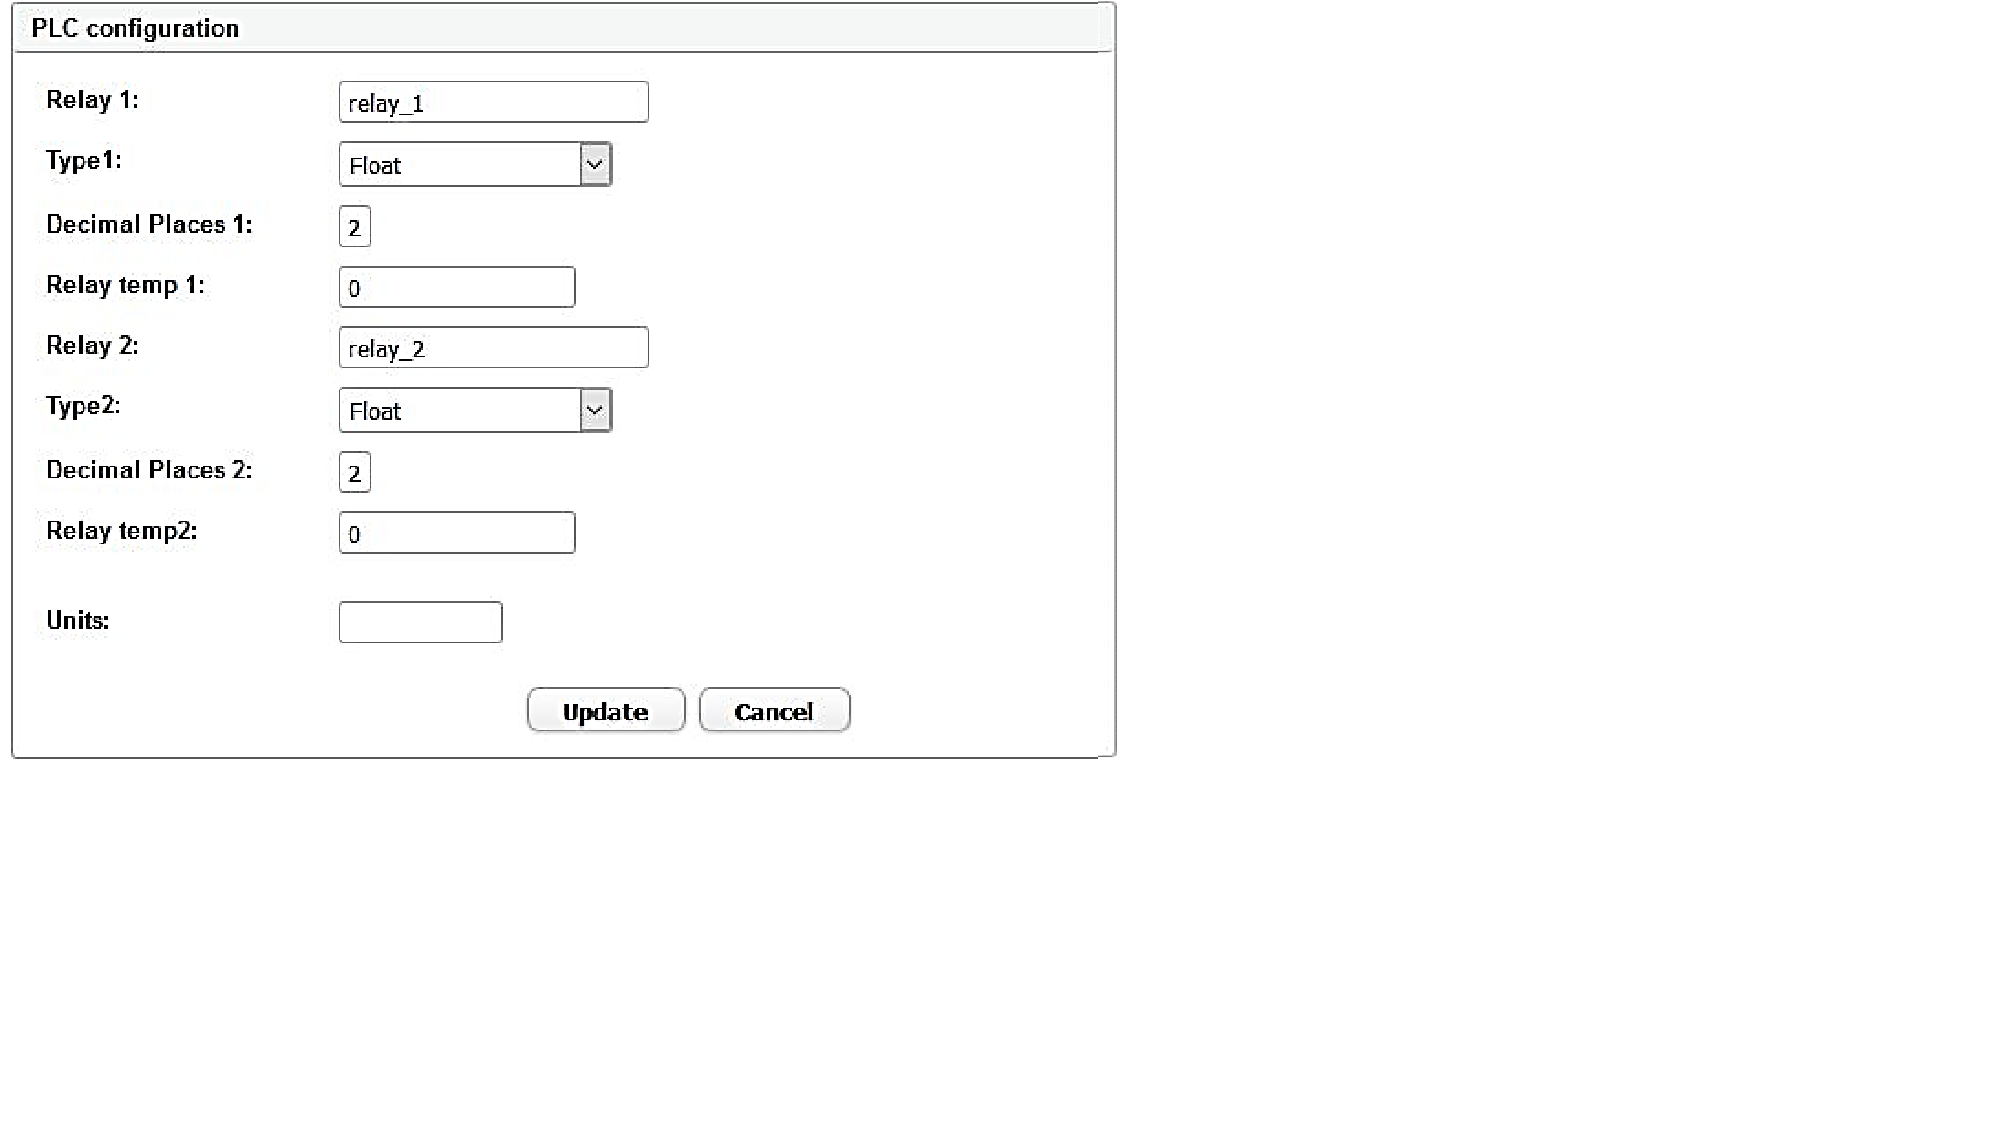
\includegraphics[trim={0 6cm 14cm 0},clip,width=\linewidth]{PLC_revised.pdf}
%     \caption{\textbf{Example configuration page.} Screenshot from the ControlByWeb x600m~\cite{controlbyweb} I/O server configuration page.}
%     \vspace{-20pt}
%     \label{fig:PLC}
% \end{figure}


\begin{figure}[t]
  \centering
    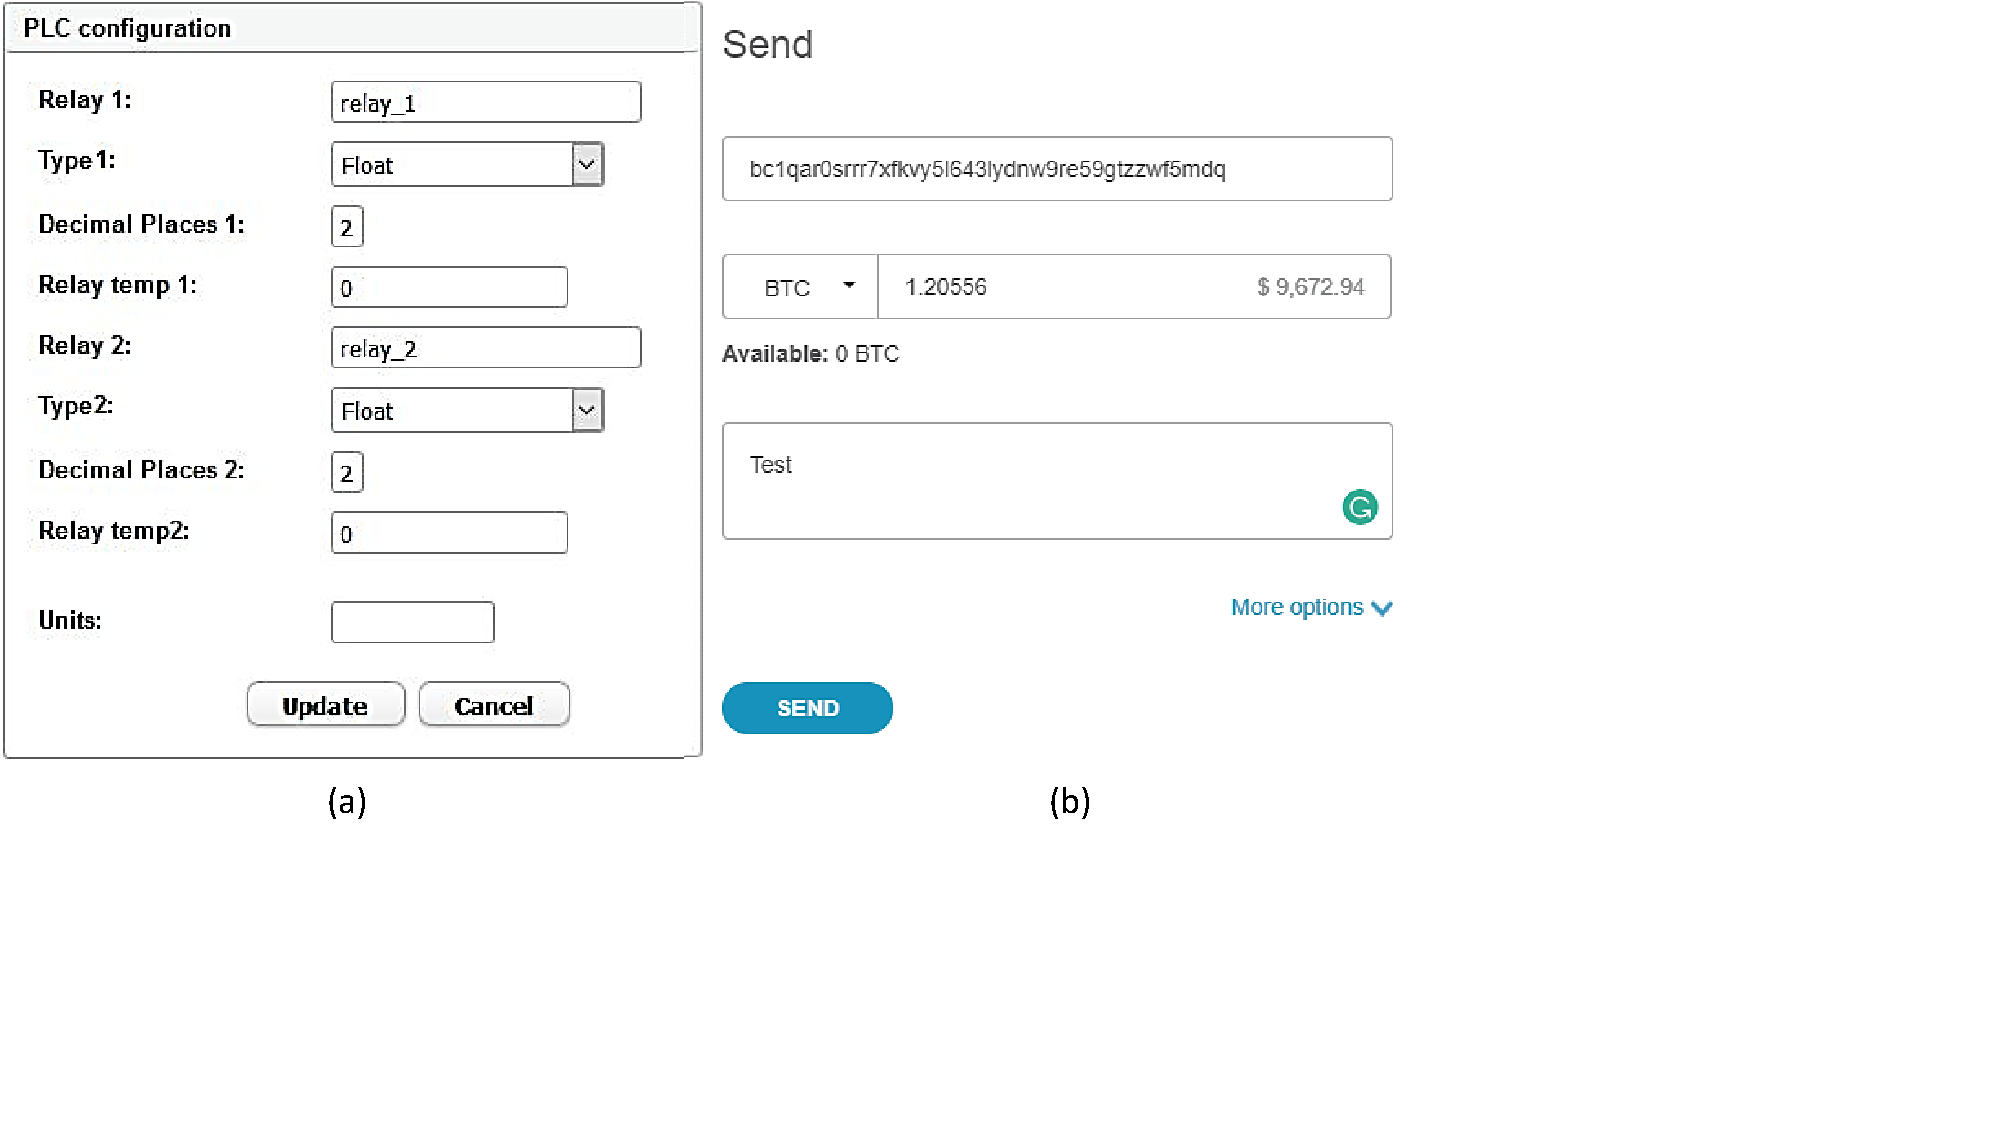
\includegraphics[trim={0 4cm 10cm 0},clip,width=\linewidth]{chapters/IntegriKey/images/config_pages.pdf}
    \caption[Example configuration page of a web-based PLC]{\textbf{Example configuration page of a web-based PLC.} Screenshot from the (a) ControlByWeb x600m~\cite{controlbyweb} I/O server configuration page, (b) web-based bitcoin wallet provide by BitGo~\cite{bitgo}. In rest of this chapter, we use the PLC server as the running example for our proposed system.}

    \label{fig:PLC}
\end{figure}


\subsection{Our Solution} 

In this chapter, we address the \emph{integrity protection} of user input in security-critical web user interfaces. Our goal is to design a solution that provides strong protection (e.g., no risk of user habituation, small TCB) and easy adoption (e.g., minimal changes to the existing systems and user experience, low deployment cost). We use remote configuration of a commercial safety-critical device (see Figure~\ref{fig:PLC} (a)) as a running example, but we emphasize that our solution is not limited to that application domain. In Section~\ref{sec:discussion_IK} we discuss how the same approach can be applied to integrity protection of various other services including financial transactions, social media posts, and email.

The basic idea behind \name is straightforward and we call this approach \emph{input trace matching}.  When the user needs to perform a security-critical web operation like configuring a PLC device or performing a cryptocurrency payment, he installs a trusted embedded device between the user input peripheral and the host platform. This device intercepts user's input events, passes them through to the host, and sends a trace of them (over a secure channel) to an authenticated remote server that compares the trace to the user input received from the host to detect input manipulation. Once the user has completed the web transaction, he can remove the embedded device from the host to preserve the user's privacy and to prevent that any subsequent input events are sent to the same server unnecessarily.

This approach can be seen as a second-factor for user input integrity protection. If the primary protection mechanism (i.e., the integrity of the host platform itself) fails, the secondary protection provided by input trace matching ensures that the target safety-critical device cannot be misconfigured.

Secure and easy adoption of this idea involves overcoming some technical challenges. The first is related to security, as an adversary that fully controls the host can execute restricted forms user input manipulation attacks, where he exchanges input values from interchangeable UI elements (e.g., two integers with overlapping ranges). Such \emph{swapping attacks} cannot be detected by the server relying on the input trace alone. Another challenge is related to deployment. Our trusted device needs to communicate with the server, but we want to avoid building an (expensive) separate communication channel into it. We further want to avoid the need to install additional software on the host that could assist in such communication. 


\myparagraph{System and tool} Based on this idea, we design and implement \name, a user input integrity protection system, that is tailored for \emph{keyboard} input, as keyboard input is sufficient for controlling many security-critical web interfaces including configuration of existing commercial safety-critical devices and execution of financial transactions.

Our system realizes the trusted embedded device as a simple USB bridge (for short \device) that is accompanied by a server-side user input matching library. To prevent subtle swapping attacks, our solution includes a simple \emph{user labeling} scheme, where the user is asked to annotate interchangeable input elements. For easy adoption, we leverage the recently introduced WebUSB browser APIs to enable communication between \device and the server in a plug-and-play manner. 

We also develop \tool, a user-interface analysis tool that helps developers to protect their web services and minimizes the added effort of users. In particular, the \tool detects input fields in web forms that require labeling and annotates the UI accordingly. 

We implemented a prototype of \device using an Arduino board and evaluated \tool using a range of existing web-based configuration UIs supported by x600m, a commercial PLC server~\cite{controlbyweb}, and several web-based Bitcoin wallets such as Bitgo~\cite{bitgo}, Bitcoin wallet~\cite{bitcoinwallet}, Coinbase~\cite{coinbase}, Coinspace~\cite{coin} and Blockchain wallet~\cite{blockchain}. Our results show that the tool can correctly process the configuration UIs of many existing security-critical web user interfaces. Our \device implementation adds a delay of $5$ ms on the processing of keyboard events and its TCB is 2.5 KLOC. 

We also conducted a preliminary user study where we simulated a swapping attack on $15$ study participants. Labeling prevented the attack in $14$ cases.


\subsection{Our Contributions} To summarize, in this chapter we make the following contributions:

\begin{enumerate}
    %\item \emph{New approach for integrity protection.} We propose input trace matching as a novel approach for integrity protection of user input on untrusted host platforms.
    \item \emph{New attack.} We identify swapping attacks as a novel form of user input manipulation against simple user input matching strategies.
    \item \name. We design and implement a user input integrity protection system that is tailored for keyboard input, prevents swapping attacks, and is easy to deploy.
    \item \tool. We develop a user interface analysis and webpage annotation tool that helps developers to protect their web services and minimizes user effort.
    \item \emph{Evaluation.} We verified that our tool can process UIs of existing safety-critical systems and cryptocurrency wallets correctly. Our experiments show that the performance delay of \name user input integrity protection is low. Our preliminary user study indicates that user input labeling prevents swapping attacks in most cases.
   %, and our preliminary user study indicates that user can perform the needed labeling. 
\end{enumerate}


\subsection{Organization of this Chapter} The rest of the chapter is organized as the following. We explain our problem in Section~\ref{sec:problemStatement_IK}. Section~\ref{sec:ourApproach} introduces our approach, Section~\ref{sec:integriKey} describes our system and Section~\ref{sec:integriTool} the UI analysis tool. We provide security analysis in Section~\ref{sec:securityAnalysis_IK}. Sections~\ref{sec:implementation_IK} and~\ref{sec:results} explain our implementation and evaluation. In Section~\ref{sec:discussion_IK} we discuss other applications for our solution. Section~\ref{sec:relatedWork_IK} reviews related work and Section~\ref{sec:conclusion_IK} concludes this chapter.




%!TEX root =  ../paper.tex
\section{SGX Background}
\label{sec:background}

Intel SGX is a TEE architecture that isolates application enclaves from all other software running on the system, including the privileged OS~\cite{sgxexplained}. Enclave's data is encrypted and integrity protected whenever it is moved outside the CPU chip. The untrusted OS is responsible for the enclave creation and its initialization actions are recorded securely inside the CPU, creating a \emph{measurement} that captures the enclave's code. Enclaves can perform local attestation, which allows one enclave to ask the CPU to generate a signed report that includes its measurement. Another enclave on the same platform can verify the validity of the report without interacting with any other external services. Enclaves can \emph{seal} data to disk, which  allows them to securely store confidential data such  that only the same enclave running in the same CPU will be able to retrieve it later.


\subsection{Remote Attestation}
\label{sec:background:attestation}

Remote attestation enables an external verifier to check whether a specific enclave has been correctly instantiated in a SGX protected environment. In the following, we describe the two main classes of remote attestation supported by Intel: i) ``enhanced privacy ID'' (EPID) attestation~\cite{epid_attestation}, and ii) the recently introduced ``data center attestation primitives'' (DCAP)~\cite{DCAP}.

\parasaverL
\myparagraph{EPID attestation.}
The EPID remote attestation is an interactive protocol between three parties: the remote verifier; the attested SGX platform; and the Intel Attestation Service (IAS), an online service operated by Intel. 
Each SGX platform includes a system service called \emph{Quoting Enclave} (QE) that has exclusive access to an attestation key. The remote verifier sends a random challenge to the attested platform, which replies with a QUOTE structure, capturing the enclave's measurement from its creation, signed with the attestation key. The verifier can then send the QUOTE to the IAS that verifies its signature and correctness, checks that the attestation key has not been revoked, and in case of successful attestation signs the QUOTE. 

The attestation key used by the QE is part of a group signature scheme called EPID that supports two signature modes: random base mode and name base mode, also called ``linkable'' mode. Both signature modes do not uniquely identify the processor to the IAS; but only a group, like a particular processor manufacturing batch. The difference between them is that the linkable signature mode allows to check whether two attestation requests came from the same CPU. 

\parasaverL
\myparagraph{DCAP attestation.} Whereas the EPID attestation variant requires connectivity to an Intel-operated attestation service, and is limited to pre-defined signature algorithms, the main goal of the DCAP attestation variant is to enable corporations to run their own local attestation services with freely chosen signature types. To achieve this, each SGX platforms is, at the time of manufacturing, equipped with a unique \emph{Platform Provisioning ID} (PPID) and \emph{Provisioning Certification Key} (PCK). Intel also provides a trusted \emph{Provisioning Certification Enclave} (PCE) that acts as a local CA and certifies custom Quoting Enclaves that can use freely-chosen attestation services and signatures.

DCAP attestation requires a trusted enrollment phase, where the enrolled SGX platform sends its PPID (in encrypted format) to a local corporate key management system that obtains a PCK certificate for the enrolled platform from an Intel-operated DCAP service. After that, the custom Quoting Enclave can create a new attestation key that is certified by the PCE enclave on the same platform. The certified attestation key can then be delivered to the corporate key management system that verifies it using the previously obtained PCK certificate. Once such enrollment phase is complete, the custom QE can sign attestation statements that can be verified by a local corporate attestation service without contacting Intel.



\subsection{Side-Channel Leakage}
\label{sec:background:attacks}

Recent research has demonstrated that the SGX architecture is susceptible to side-channel leakage. Secret-dependent data and code access patterns can be observed by monitoring shared physical resources such as CPU caches~\cite{sgxcache,gotzfried2017cache,moghimi2017cachezoom} or the branch prediction unit~\cite{lee2017inferring}. The OS can also infer enclave's execution control flow or data accesses by monitoring page fault events~\cite{xu2015controlled}. Many such attacks can be addressed by hardening the enclave's code, e.g., using cryptographic implementations where the data or code access patterns are independent of the key.

The recently discovered system vulnerabilities Spectre~\cite{Kocher2018spectre} and Meltdown~\cite{Lipp2018meltdown} allow application-level code to read memory content of privileged processes across separation boundaries by exploiting subtle side-effects of transient execution. The Foreshadow attack~\cite{foreshadow-usenix18} demonstrates how to extract SGX attestation keys from processors by leveraging the Meltdown vulnerability. 

\parasaverL
\myparagraph{Microcode updates.}
During manufacturing, each SGX processor is equipped with hardware keys. When SGX software is installed on the CPU for the first time, the platform runs a provisioning protocol with Intel. In this protocol, the platform uses one of the hardware keys to demonstrates that it is a genuine Intel CPU running a specific microcode version and it then then joins a matching EPID group and obtains an attestation key~\cite{epid_attestation} (or a signing key for the PCE enclave). 

Microcode patches issued by Intel can be installed to processors that are affected by known vulnerabilities such as the above mentioned Foreshadow attack. When a new microcode version is installed, the processor repeats the provisioning procedure and joins a new group that corresponds to the updated microcode version and obtains a new attestation key which allows IAS to distinguish attestation signatures that originate from patched processors from attestation signatures made by unpatched processors~\cite{epid_attestation}.
%!TEX root =  ../paper_NDSS.tex

\section{Relay Attack Analysis}
\label{sec:problemStatement}

In this section, we provide an analysis of relay attacks on SGX. 

\begin{figure}[t]
 \centering
  %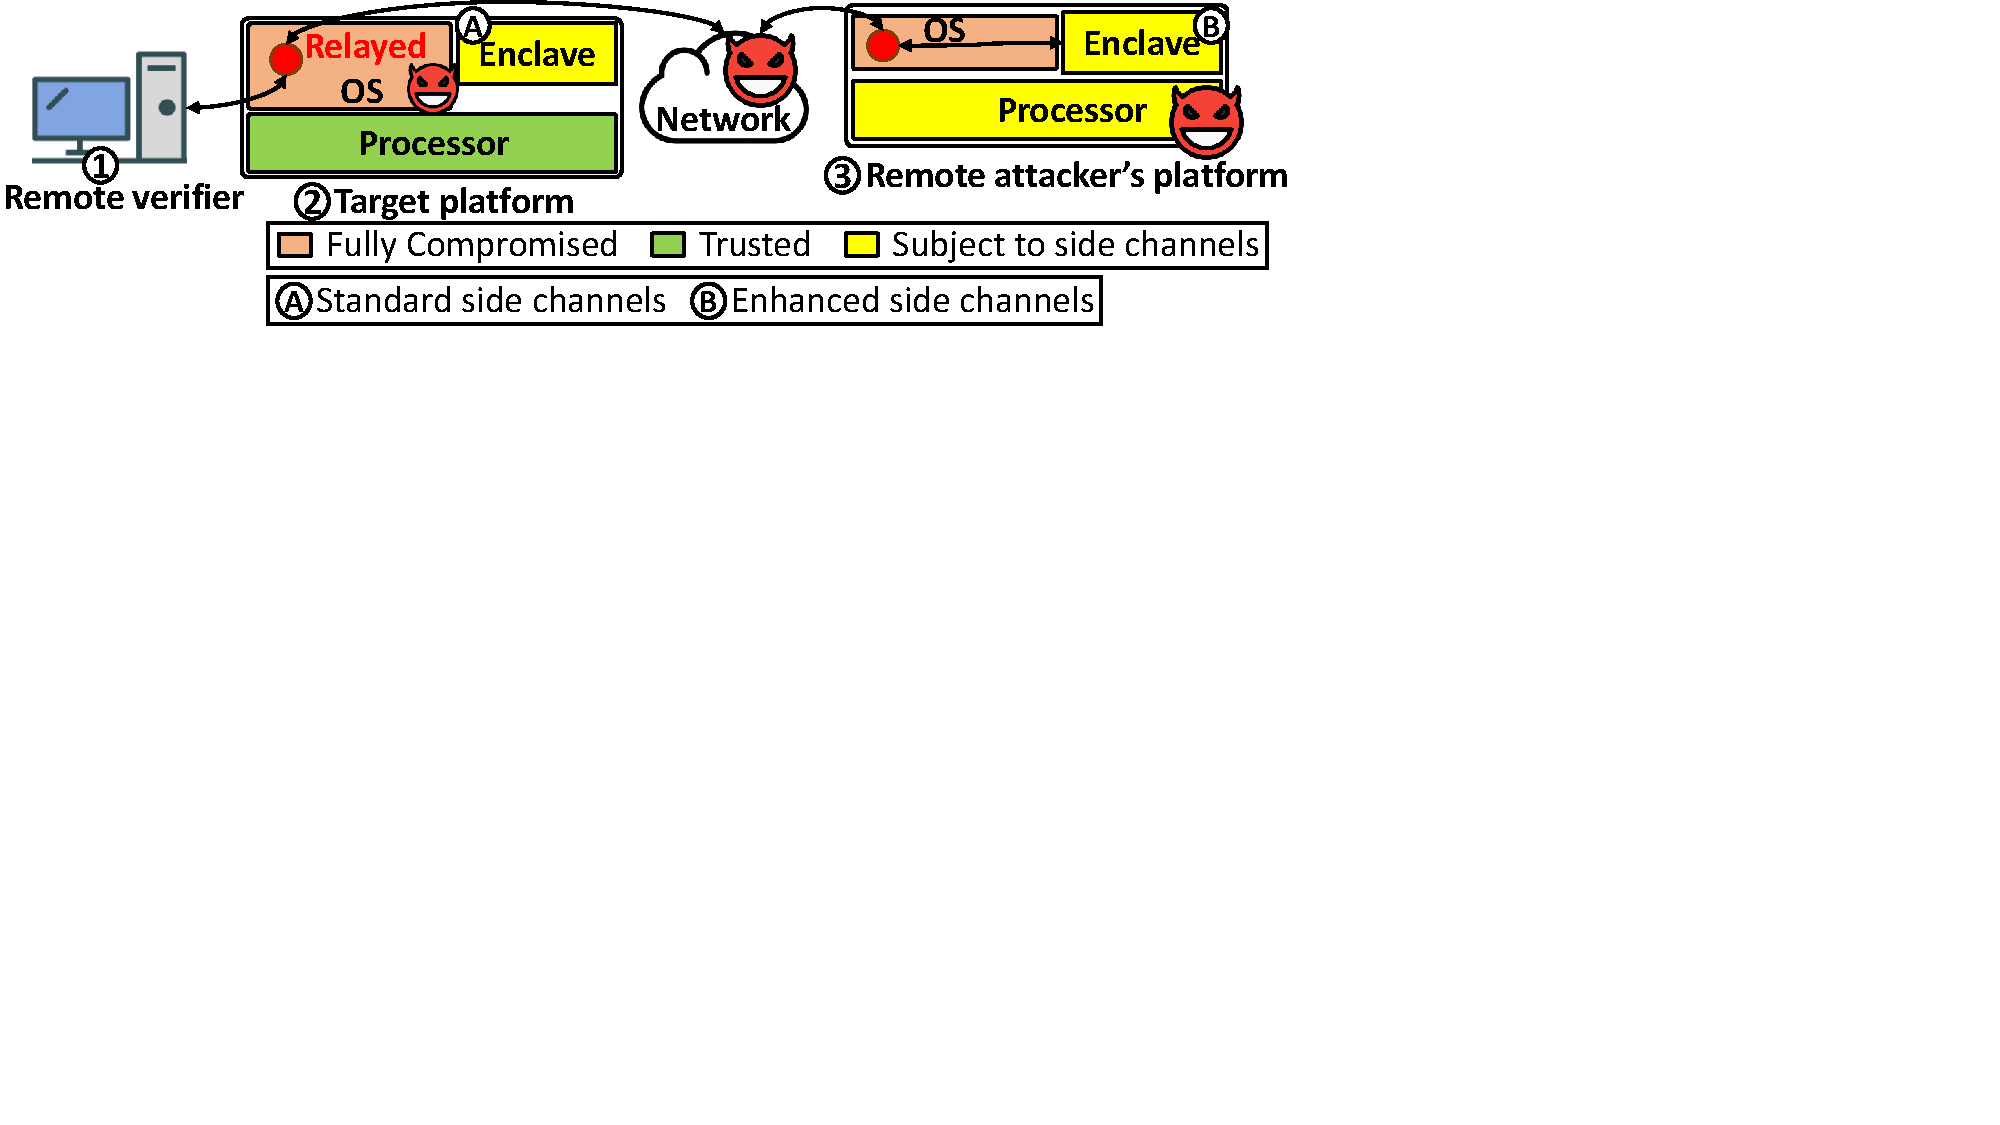
\includegraphics[trim={0 13.4cm 11cm 0},clip,width=\linewidth]{relayAttack.pdf}
  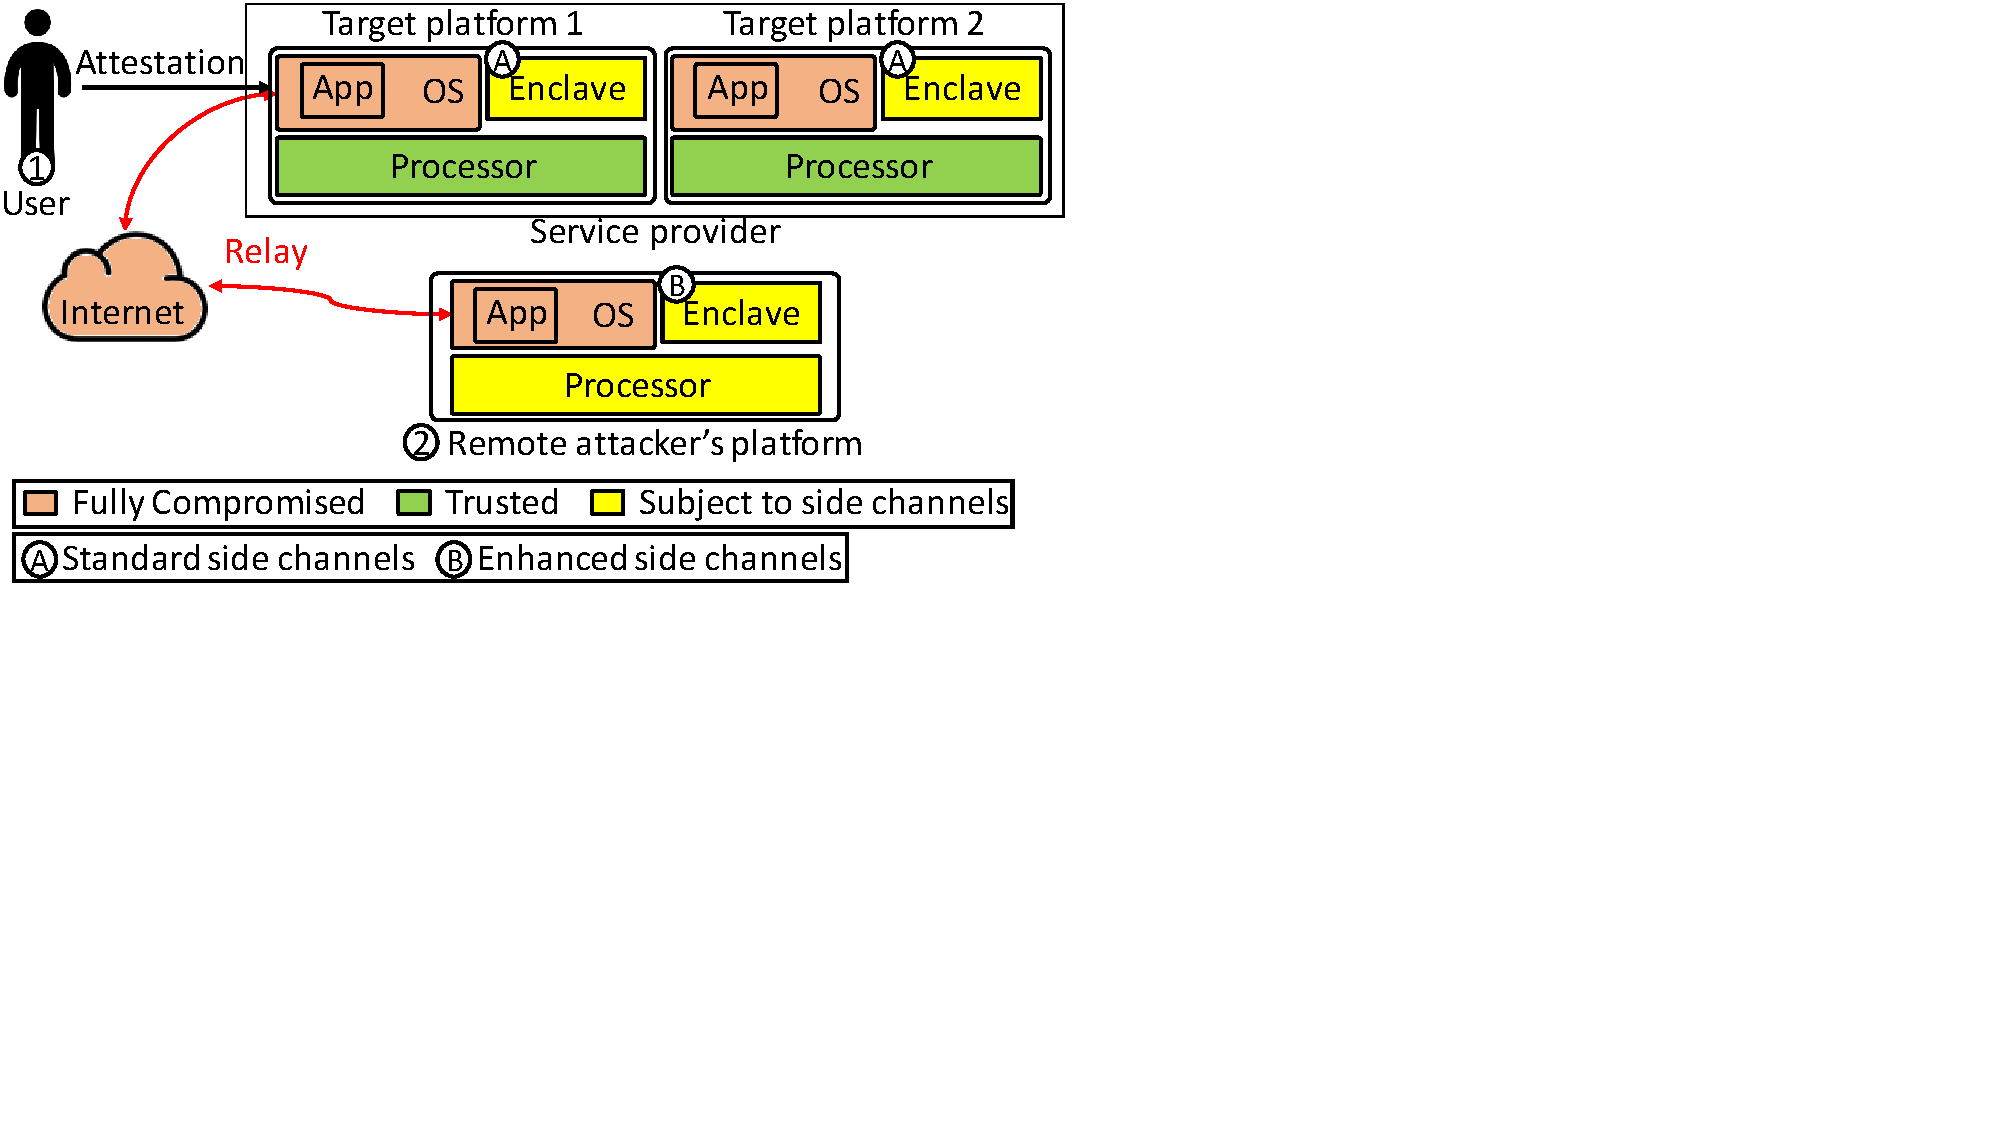
\includegraphics[trim={0cm 9cm 15.8cm 0},clip,width=0.75\linewidth]{chapters/ProximiTEE/figures/relayAttack2.pdf}
 \caption[Relay attack]{\textbf{Relay attack.} The adversary redirects attestation to his own platform which gives him increased (side-channel and kernel-level) abilities to attack the attested enclave.}

 \label{fig:SystemModel}
\end{figure}


\subsection{Relay Attacks}
\label{sec:problemStatement:systemAttackerModel}

We consider a system model shown in Figure~\ref{fig:SystemModel} that consists of three parties: the target platform, the remote verifier, and the attacker's platform. The remote verifier is a trusted party that wishes to connect and attest to a specific SGX platform. The target platform is the SGX platform to which the remote verifier intends to connect. Finally, the attacker's platform is a platform owned by the attacker that is connected to the target platform through the Internet.



\subsubsection{Adversary model} We consider the following adversary model that we call the \emph{relay attacker}. The relay attacker controls the OS and all other privileged software on the \emph{target} platform at least \emph{temporarily}, in particular at the time of the remote attestation. The OS compromise on the target platform may be later detected and disinfected. We consider the case in which the target platform resides in a data center or otherwise in a facility with restricted physical access. The attacker hence \emph{does not} have physical access to the target platform (or any other co-located platform in the same facility). %The relay attacker cannot extract attestation or sealing keys from the target platform.

The relay attacker controls the OS and all other privileged software on the attacker's platform \emph{permanently} and has physical access to that platform. The attacker also controls the network between the target platform and his platform. At the time of the attestation, the adversary has not been able to extract attestation or sealing keys from his platform or any other SGX processor.


\subsubsection{The process of the relay attack} The relay attacker can redirect the attestation requests intended for the target platform to his platform, as shown in Figure~\ref{fig:SystemModel}. This is a realistic attack for two reasons. First, in the SGX attacker's model the adversary is allowed to control the OS and can hence easily redirect any network request the target platform receives. Second, even if the attacker cannot compromise the OS in the target platform, it might be able to exploit some vulnerability of the untrusted application managing the enclave. The exploit might allow the attacker to manipulate the application's control flow to redirect attestation request to any platform he desires.




\begin{figure}[t]
\footnotesize
    \centering
    \begin{tikzpicture}[
solved/.style={rectangle,draw,fill=purple!40, rounded corners, align=center},
not/.style={rectangle, draw,fill=orange!60, rounded corners, align=center},
neutral/.style={rectangle, draw, rounded corners, align=center, fill=black!5},
sibling distance=12em]]
    \node[neutral](root) {SGX attacks}
    child { node[not, yshift=13pt] (name) {Attacks enabled by \\ leaked attestation keys ~\cite{foreshadow-usenix18}} }
    child { node[neutral, yshift=13pt] (app) {Side-Channels \\ on application enclave}
      child { node[neutral, yshift=0pt] (soft) {Software/digital}
		child { node[solved, yshift=-10pt] (pe) {Privilege\\ escalation}}      
        child { node[not, right=1.5em of pe,yshift=-10pt] (a) {Case (A) in Figure~\ref{fig:timeLine}:\\Complement of Case (B)}}
        child { node[solved, right=1.5em of a, yshift=-12pt] {Case (B) in Figure~\ref{fig:timeLine}:\\
            \begin{tabular}{rl}
                Target platform:& secure\\
                Attacker's platform:& vulnerable\\
            \end{tabular}}} }
      child { node[solved, yshift=12pt] (physical) {Physical} } };
      
    %\node[below=0cm of name] {Foreshadow~\cite{foreshadow-usenix18}};
    \node[below=0cm of physical](power) {Power analysis~\cite{wang2006covert}};
    \node[below=-5pt of power](EM) {EM radiation~\cite{gandolfi2001electromagnetic}};
    \node[below=-5pt of EM](ac) {Acoustic~\cite{shamir2004acoustic}};
         
    \node[left=10pt of soft](page) {Page fault~\cite{xu2015controlled}};
    \node[above=-3pt of page](cache) {Cache~\cite{dall2018cachequote,gotzfried2017cache,sgxcache,moghimi2017cachezoom}};
    \node[below=-2pt of page](branch) {Branch prediction~\cite{lee2017inferring}};
    %\node[below=-5pt of branch](synch) {Synchronization~\cite{asyncshock}};
      
    \node[solved, right=4em of root,  minimum size=3mm](l1) {};
    \node[right=0cm of l1](l1_1) {Enabled by relay};
    \node[not, below=1pt of l1, minimum size=3mm](l2) {};
    \node[right=0cm of l2](l2_1) {Independent of relay};
    
    \end{tikzpicture}
    
    \caption[Relay attack implications]{\textbf{Relay attack implications.} The tree shows the types of attacks that are enabled by  redirection and ones that are independent of relay.}
    \label{fig:relayTree}
\end{figure}

            
\subsection{Relay Attack Implications}
\label{sec:problemStatement:implication}

Although relay attacks have been known for a long time~\cite{parno2008bootstrapping}, their implications to modern TEEs like SGX have not been carefully analyzed. Next, we perform the first such analysis.

The main consequence of attestation redirection is that it \emph{increases the adversary's ability to attack the attested enclave} through side-channels which are a well-known limitation of SGX (see Section~\ref{sec:background:attacks}). In Figure~\ref{fig:relayTree} we highlight two major classes of attacks: those that are only possible by first performing a relay attack, which we denote as ``enabled by relay'', and those that can be done whether or not the attacker also does a relay attack, which we call ``independent of relay.''


\subsubsection{Attacks using leaked attestation keys} Our first observation is that attacks based on leaked attestation keys (e.g., ones obtained through the Foreshadow attack~\cite{foreshadow-usenix18}) are independent of relaying. If the adversary has obtained a valid and non-revoked attestation key, he can emulate an SGX processor on the target platform and obtain any secrets provisioned to it.


\subsubsection{Physical side channels} One major benefit of the relay, from the adversary's point of view, is that it enables \emph{physical} side-channel attacks against application enclaves. Once a secret has been provisioned to the attacker's platform, she has as much time as she likes to perform the attack. Some examples of physical side-channel attacks are acoustic, electric and electromagnetic monitoring, which have been shown to be both effective and inexpensive means to extract secrets from modern PC platforms (see~\cite{genkin2016physical} for a summary of known attacks). Since the adversary does not have physical access to the target platform, such attacks are clearly not possible without relay. Hardening programs like enclaves against physical side channels is difficult and currently an open problem~\cite{genkin2016physical}. Therefore, developers cannot easily defend their enclaves against physical side channels that are enabled by attestation redirection.


\subsubsection{Privilege escalation for digital side channels}
Another possible benefit of relay attacks is that it may enable \emph{privilege escalation}. In cases where the adversary has only compromised the user-space application that manages the enclave, and not the OS, the application can redirect the attestation to the attacker's remote platform where he controls the OS as well. In such cases, the relay enables \emph{digital} side-channel attacks that require system privileges. Several such attacks have been recently demonstrated against SGX~\cite{moghimi2017cachezoom, sgxcache, gotzfried2017cache}.


\begin{figure}[t]
\footnotesize
    \centering
    \begin{tikzpicture}[
    solved/.style={rectangle,draw,fill=purple!40, rounded corners, align=center},
    relayNode/.style={circle,draw,fill=red!40, align=center},
    edge from parent/.style={draw,-latex},    
    neutral/.style={rectangle, draw, rounded corners, align=center, fill=black!5},
    not/.style={rectangle, draw,fill=orange!60, rounded corners, align=center},
    sibling distance=12em]]
    
 
 
 \node[] (targetA) {\textbf{Target}};
 \node[right=33pt of targetA] (attackA) {\textbf{Attacker}};
 \node[below=0 of attackA] (dummy) {};
 
  
 \node[neutral, below=0.1cm of targetA](root1) {OS compromised};    
 \node[relayNode, below = 1em of root1] (relay1) {Relay};
 \node[neutral, right = 3em of relay1] (attestation1) {Attest enclave};
 \node[neutral, below = 1em of relay1] (discovery1) {New attack\\ discovery};        
  \node[neutral, below = 2.2em of attestation1] (discoveryAttack1) {New attack\\ discovery};  
 \node[neutral, below = 0.6em of discoveryAttack1] (provisioning1) {Secret\\ provisioning};
 \node[neutral, below = 3.5em of discovery1] (cleanup1) {OS cleanup};    
 \node[below = 3em of cleanup1] (end) {};      
 \node[not, below = 2em of provisioning1] (independent) {Independent of relay};
 
 
  \draw[->, thick] (root1) edge[] node{} (relay1);
 \draw[->, thick] (relay1) edge[] node{} (discovery1);
 \draw[->, thick] (relay1) edge[] node{} (attestation1);
 \draw[->, thick] (attestation1) edge[] node{} (discoveryAttack1);
 \draw[->, thick] (discovery1) edge[] node{} (cleanup1); 
 \draw[->, thick] (discoveryAttack1) edge[] node{} (provisioning1);
 \draw[->, thick] (provisioning1) edge[] node{} (independent);
 \draw[->, thick] (dummy) edge[] node{} (attestation1);
 \draw[->, thick] (cleanup1) edge[] node{} (end);
  \node[below=0cm of independent] {Case (A)};
 

 \node[right=0.79cm of attackA](point1){};
 \node[below=19em of point1](point2){Time};
 \draw[->] (point1) edge[] node{} (point2);
 
 \node[right=50px of attackA] (targetB) {\textbf{Target}};
 \node[right=37px of targetB] (attackB) {\textbf{Attacker}};
  \node[below=0 of attackB] (dummy1) {};
 
 %\draw ($(attackA)!0.5!(targetB)$) -- ($(attackA)!0.5!(targetB) - (0, 5)$);    
 \node[neutral, below=0.1cm of targetB](root) {OS compromised};
 \node[relayNode, below = 1em of root] (relay) {Relay};
 \node[neutral, right = 3.5em of relay] (attestation) {Attest enclave};
 \node[neutral, below = 0.6em of attestation] (provisioning) {Secret\\ provisioning};
 \node[neutral, below = 2em of relay] (cleanup) {OS cleanup};
 \node[neutral, below = 1em of cleanup] (discovery) {New attack\\ discovery};   
 \node[below = 3.5em of discovery] (end1) {};        
 \node[neutral, below = 2.5em of provisioning] (discoveryAttack) {New attack\\ discovery};           
 \node[solved, below = 1.7em of discoveryAttack] (attack) {Enabled by relay}; 
 
 
 \draw[->, thick] (root) edge[] node{} (relay);
 \draw[->, thick] (cleanup) edge[] node{} (discovery); 
 \draw[->, thick] (discoveryAttack) edge[] node{} (attack);
 \draw[->, thick] (relay) edge[] node{} (cleanup);  
 \draw[->, thick] (provisioning) edge[] node{} (discoveryAttack); 
 \draw[->, thick] (relay) edge[] node{} (attestation);
 \draw[->, thick] (attestation) edge[] node{} (provisioning);        
 \draw[->, thick] (dummy1) edge[] node{} (attestation);
 \draw[->, thick] (discovery) edge[] node{} (end1);
\node[below=0cm of attack] {Case (B)};
   

                         
    \end{tikzpicture}
    \caption[Relay timing of attack]{\textbf{Relay timing of attack.} In Case A the attack success is independent of relay. In Case B attestation redirection enables the attack.} 
    \label{fig:timeLine}
\end{figure}


\subsubsection{Attacks that depend on timing of events.}    
The third, and perhaps the most subtle, implication of relay is that it can also enable software-based side-channel attacks that would not be possible to launch on the target platform due to \emph{timing of certain events}. These events include, but are not restricted to the provisioning of secrets to the enclave, the possible disinfection of the target platform from malicious software, and the discovery of a new side-channel attack. 

We group the relative ordering of these events into two cases: A and B. Case A covers event sequences that only lead to attacks which are independent of relay and Case B covers event sequences in which redirection gives extra capabilities to the adversary. Below, and in Figure~\ref{fig:timeLine}, we provide examples of sequences belonging to these two cases:

\begin{enumerate}
    \item[]\emph{Case A: independent of relay.} A digital side-channel is independent of relay if the adversary could perform it on the target platform as well. An example of such case is shown th timeline depicted in Figure~\ref{fig:timeLine}, where a new attack is discovered after secret provisioning but before the target platform OS is disinfected.
    

    \item[]\emph{Case B: attack enabled by relay.} Case B is reached whenever it occurs that by using a side channel the enclave is exploitable on the attacker's platform, but not on the target platform. 
    %In this case, by having the foresight to provision the enclave on its platform, the attacker has the possibility to launch an attack on an enclave that would otherwise be secure on the target platform. 
    A timeline of such case is shown in Figure~\ref{fig:timeLine}, where at the time of attestation and secret provisioning, the enclave is hardened against all known digital side-channel attacks (using tools like Raccoon~\cite{raccoon}, ZeroTrace~\cite{zerotrace} or Obfscuro~\cite{obfscuro}). After secret provisioning, the OS compromise is detected and cleaned. Later, a new side-channel attack vector (that is not prevented by the used tools) is discovered. If the adversary performed redirection and the secret was provisioned to the attacker's machine, the new side channel is exploitable. Without the relay, the attack is not possible.
    

\end{enumerate}


\subsection{Limitations of Known Solutions}
\label{sec:problemStatement:limitations}

Next, we review commonly suggested solutions and their limitations.

\subsubsection{Trust on first use} 
A common ``solution'' in the research literature is to rely on \emph{trust on first use} (TOFU)~\cite{tofu}. Simple TOFU solutions assume that the OS is clean at the time of attestation or perform attestation only immediately after fresh OS installation. Both of these approaches have obvious security and deployment problems. OS re-installation is not always possible and trusting the OS, even if momentarily, is undesirable (and violates the SGX's trust model).

\subsubsection{SGX attestation variants.}
As we explain in Section \ref{sec:background:attestation}, SGX supports different variants of remote attestation. Unfortunately, none of these schemes prevents relay attacks without some form of TOFU assumption.

\begin{enumerate}
	\item \emph{The EPID attestation scheme} is based on group signatures, and thus the remote verifier cannot distinguish between attestation responses that are received from the expected target platform or the adversary's platform. To accept a successful attestation, the remote verifier must rely on trust on first use. 

	\item \emph{The linkable EPID attestation mode} allows the remote verifier to check if he has attested the same platform before, but the first attestation protocol run is vulnerable to relay attacks, and therefore also in this case the remote verifier must assume TOFU. 

	\item \emph{The DCAP scheme} allows corporations to operate their own local attestation services after an enrollment phase. However, if the adversary controls the target platform during the enrollment, he can replace the enrolled platform identifier PPID with the identifier of his own platform PPID' and enroll the adversary's platform instead. Thus, also the DCAP variant scheme requires trust on first use. In addition, the entire corporate key management system must be trusted at the time of the enrollment (and after it).
\end{enumerate}


\subsubsection{Non-anonymous attestation.}
Because SGX's attestation protocol support anonymity features, like the EPID signature scheme, one may think that relay attacks are caused by such privacy protection mechanism. However, such reasoning is incorrect. Even if all anonymity features would be removed from attestation, the problem of relay attacks would still persist. The root cause of relay attacks is that certified keys can be securely installed to processors at the time of manufacturing, but the processor ownership by private individuals or companies is established much later. Therefore, common PKI mechanism do not eliminate relay attacks --- unless the processor manufacturing and distribution model is completely changed such that factories start to manufacture and certify customers-specific processors batches on demand (which would be very expensive).


\subsubsection{Other TOFU variants.}
Recent research papers use slightly different TOFU variants. For example, the \textsc{Rote} system~\cite{matetic2017rote} assumes fresh OS installation at system initialization time and for each used platform it requires a local administrator to input a credential to the enclaves. As another example, in the \textsc{VC3} system~\cite{schuster2015vc3} enclaves generate a public/private key pair at the time of trusted initialization, output the public key and seal the private key. The public key can be sent to a trusted authority for certification, which then enables clients to securely connect to enclaves. Both of these solutions essentially avoid insecure attestation by pre-authorizing known enclaves during a setup phase that is assumed trusted. 

In general, TOFU solutions suffer from the following limitations:

\begin{enumerate}
  \item \emph{OS re-installation:} Forcing users or administrators to re-install the OS is not always possible. 
  
  \item \emph{Manual configuration:} Manual interaction tasks, such as an administrator that needs to enter credentials to enclaves during initialization, complicates platform enrollment, especially in scenarios like data centers with many enrolled platforms.

  \item \emph{Pre-defined enclaves:} Solutions that only work with enclaves that are known at the time of initialization are not applicable to scenarios like cloud computing platforms where users need to install new enclaves after platform installation. 

  \item \emph{Large temporary TCB:} Modern operating systems have a large TCB and trusting the OS even temporarily is unideal.

  \item \emph{Online authorities:} Solutions where a trusted authority needs to either certify or revoke new enclaves typically require that the authorities are online, which increases their attack surface.
\end{enumerate}



\section{\name}
\label{sec:systemDesignMain}

Our goal is to design a solution that addresses the above limitations of previous solutions. In short, our solution should be \emph{secure} (no TOFU assumption, small TCB, no online authorities) and \emph{easy to deploy} (no OS re-installation, manual configuration, or pre-defined enclaves). In this section, we provide an overview of our approach, outline possible use cases, describe our solution in detail, and analyze its security.

\subsection{Approach Overview}

We propose a hardened SGX attestation scheme, called \name, based on a simple embedded device that we call \device. The embedded device is attached to the target platform over a local communication interface such as a USB. 

% as shown in  Figure~\ref{fig:approach}. %Using this approach, we propose a hardened attestation mechanism to address the relay attacker defined in Section~\ref{sec:problemStatement:attackerModel}.

Our main idea is to use the combination of such a trusted device and \emph{proximity verification} to prevent relay attacks. In our solution, the \device device verifies the proximity of the attested enclave, and after successful proximity verification, it facilitates the creation of a secure channel between the remote verifier and the attested enclave. 

After the initial attestation, the device periodically checks proximity to the attested enclave. The established secure channel is contingent on the physical presence of the embedded device on the target machine, and it stays active only as long as the device is plugged in. The act of detaching the device automatically revokes the attested platform without any interaction with a trusted authority. Thus, our solution enables secure \emph{offline} enrollment and revocation. 

To use our solution, enclave developers use a simple API that facilitates communications between the enclave and the device. 


\myparagraph{Security assumptions}
%\label{sec:ext-attacker-model}
In our solution, the \device device is a trusted component. We deem this choice reasonable since it implements only the strictly necessary functions, and therefore, it has significantly smaller software TCB, attack surface, and complexity compared to a general-purpose commodity OS. We assume that its issuer certifies each embedded device prior to its deployment, and such certification can take place fully offline.

Concerning the security of the \device device we employ the same attacker model introduced in Section~\ref{sec:problemStatement} for enclaves. While the user's device and its private keys are never exposed to the attacker, another similar device can be in the physical possession of the attacker, which has as much time as she wants to fully compromise it (run arbitrary code and extract keys). 


\subsection{Example Use Cases}
\label{sec:use-cases}

Our solution is targeted to scenarios where the benefits of more secure attestation outweigh the deployment cost of a simple embedded device. Here, we outline three example cases.  

\myparagraph{Data center} In our first example, we consider a cloud platform provider that attaches \device to a server in a specific data center and makes the public key of the connected device known to the users of the service. Our approach is particularly well suited to cloud computing models where customers rent dedicated computing resources like entire servers. In such a setting, our solution ensures that the cloud platform customer outsources data and computation to a server that resides in a specified location. Enforcing location may be desirable to meet increasing data protection regulation that defines how and where data can be stored, even if protected by TEEs such as SGX. Revocation (e.g., when a server is relocated to another data center or function) can be realized by merely detaching \device.

\myparagraph{Permissioned blockchain} Our second case is a setting in which a trusted authority initializes a set of validator nodes for a permissioned and SGX-hardened blockchain. 
The trusted authority issues one \device for each organization that operates one of the validator nodes, which allows secure attestation of the validator platforms. Organizations are free to upgrade their computing platforms by attaching the \device to a new platform which automatically revokes the old platform without the need to interact with a trusted authority. Furthermore, since \device can only be active on one platform at a time, such a deployment enables the authority to control the identities used in a (Byzantine) blockchain consensus process.



\myparagraph{HSM-protected keys} Our last case is the management of HSM-protected keys from an attested enclave. Such deployment enables the secure and flexible realization of various access control policies, implemented as attested enclaves. \name guarantees that only an enclave in the proximity of the HSM can control its keys. Such a solution provides a high level of protection because, at no point in time, the HSM keys are directly accessible by the enclave (which may be vulnerable to side-channel attacks) or by the untrusted OS.


\subsection{Solution Details}
\label{sec:systemDesign}


Now, we explain the \name attestation mechanism in detail.


\myparagraph{Attestation protocol} 

Figure~\ref{fig:systemSetUp} illustrates the attestation protocol that proceeds as follows:


\begin{figure}[t]
 \centering
  %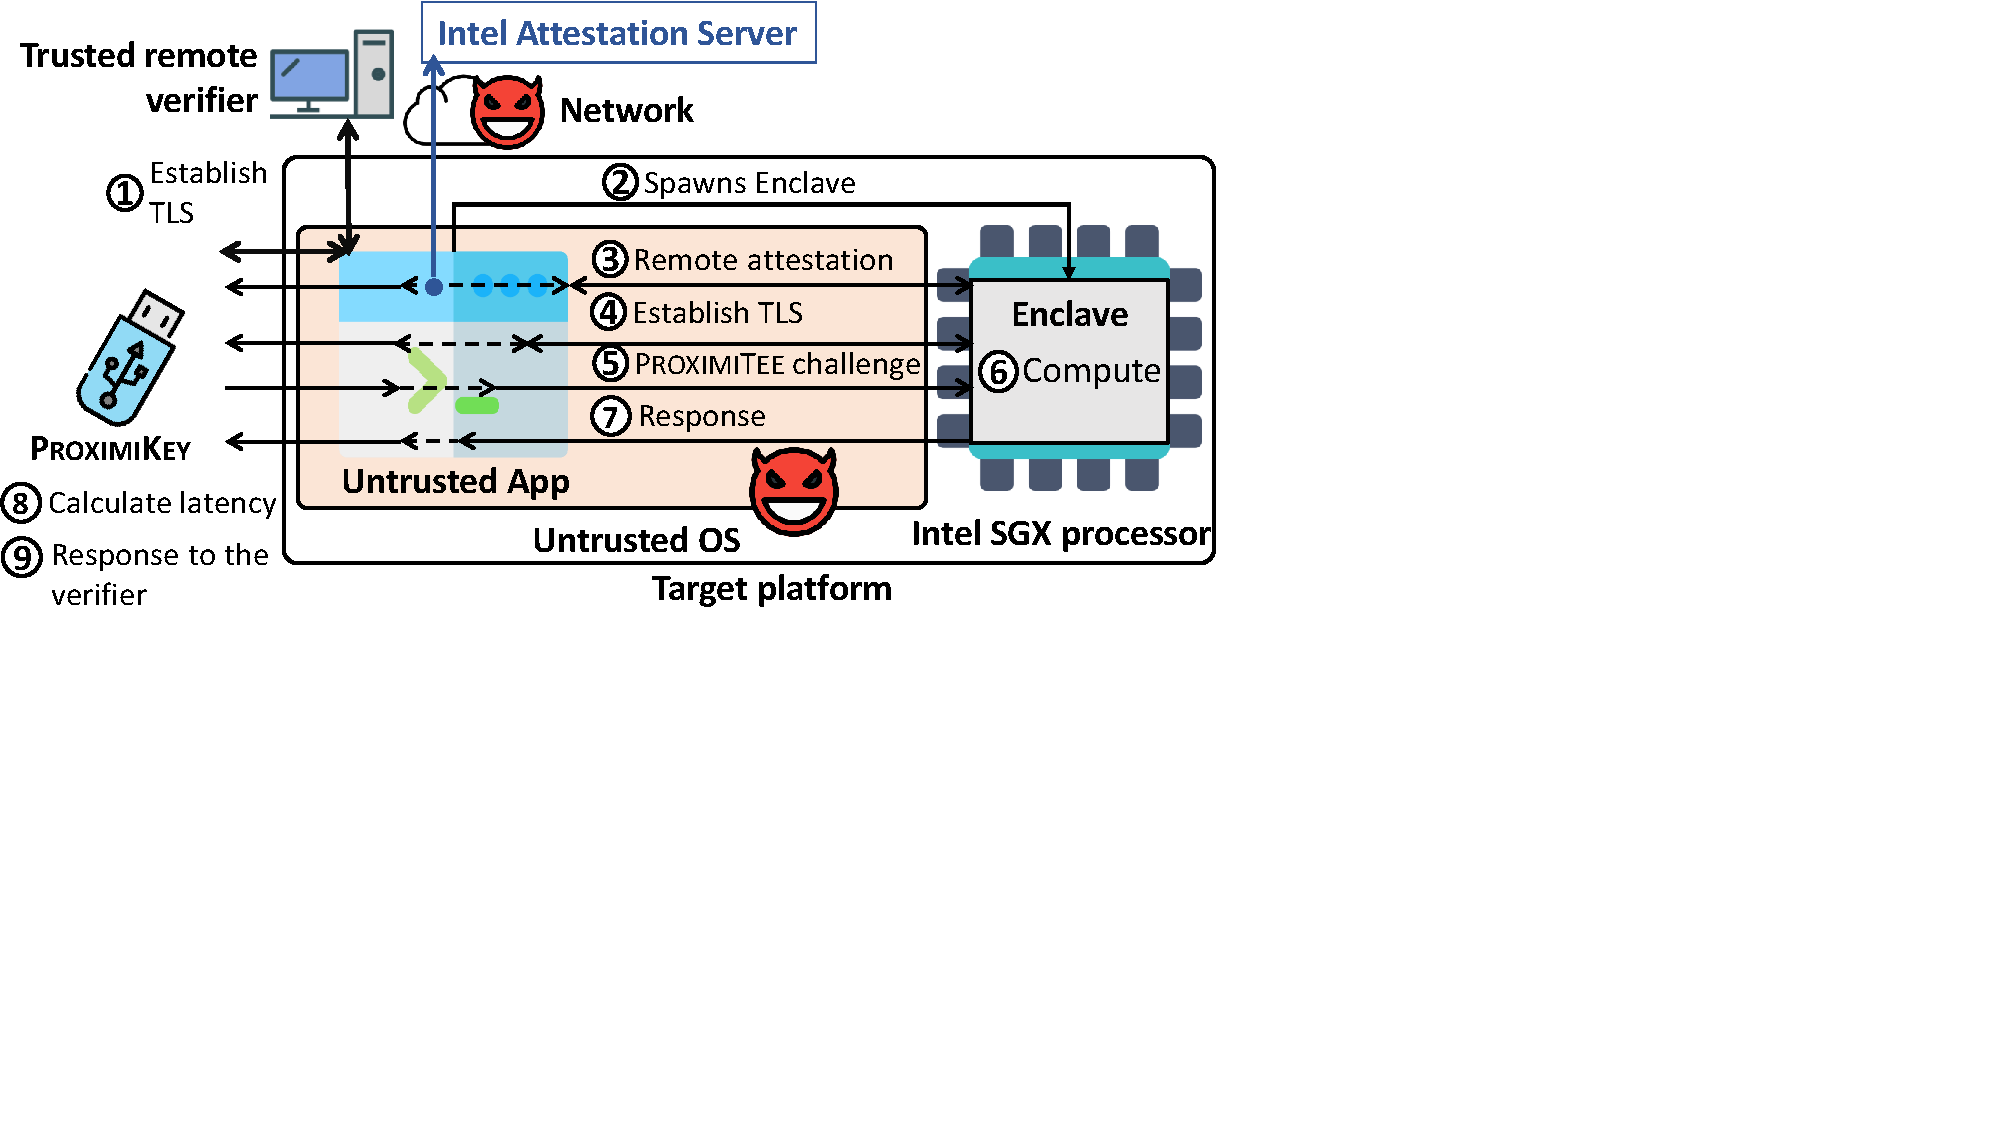
\includegraphics[trim={0 8.7cm 13.2cm 0},clip,width=\linewidth]{chapters/ProximiTEE/figures/proximiteeMain.pdf}
  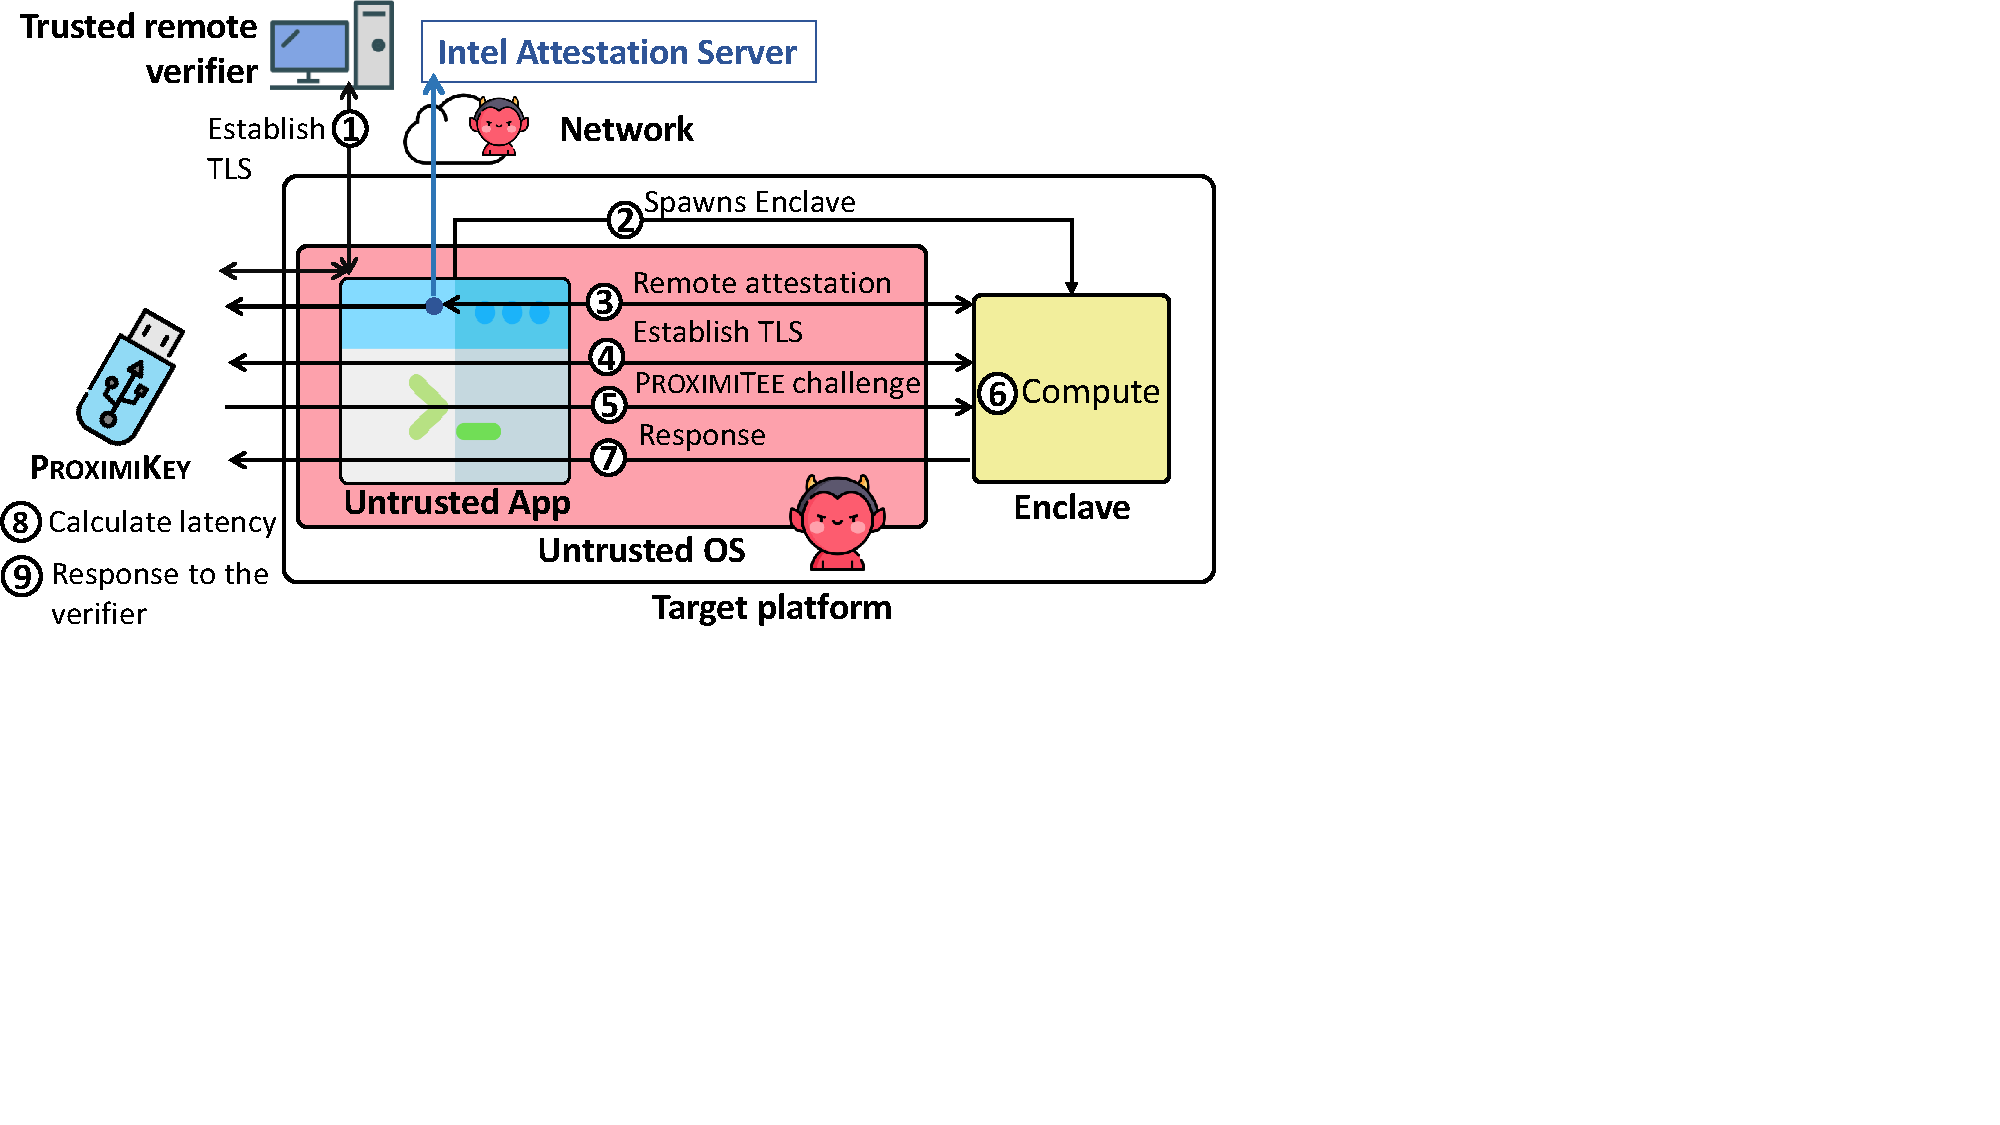
\includegraphics[trim={0 8cm 13.2cm 0},clip,width=\linewidth]{chapters/ProximiTEE/images_new/distance_bound.pdf}
 \caption[\name attestation]{\textbf{\name attestation.} The remote verifier establishes a secure channel to the \device device that first attests the enclave and then verifies its proximity.}
 	\label{fig:systemSetUp}
\end{figure}

\begin{enumerate}%
 
  \item[\one] The remote verifier establishes a secure channel (e.g., \tls) to the certified \device. An assisting but untrusted user-space application facilitates the connection on the target platform, acting as a transport channel between the remote verifier and the \device (and later also the enclave). As part of this first step, the remote verifier specifies which enclave should be executed.%

  \item[\two] The untrusted application creates and starts the attestation target enclave.%

  \item[\three] \device performs the standard remote attestation to verify the code configuration of the enclave with the help of the IAS server or using a custom DCAP procedure (see Section~\ref{ch:background:SGX:remote}). In the attestation protocol, the device learns the public key of the attested enclave.%

  \item[\four] \device establishes a secure channel (e.g., \tls) to the enclave using that public key.

  \item[\five] \device performs a distance-bounding protocol that consists of $n$ rounds, where each round is formed by steps \five to \eight.
  %(see Figure~\ref{fig:challengeResponse}).
  At the beginning of each round \device generates a random challenge $r$ and sends it to the enclave over the TLS channel.

  \item[\six] The enclave increments the received challenge by one $(r+1)$.

  \item[\seven] The enclave sends a response ($r+1$) back to the \device over the \tls channel.

  \item[\eight] \device verifies that the response value is as expected (i.e., $r+1$) and checks if the latency of the response is below a threshold (\connect). Successful proximity verification requires that the latency is below the threshold for at least $k \times n$ responses, where $k \in (0, 1]$ is a percentage of the total number of responses $n$.

  \item[\nine] If proximity verification is successful, the \device notifies the remote verifier over the \tls channel (constructed in step \one). The verifier starts using the \device TLS channel to send messages to the enclave.
\end{enumerate}


\myparagraph{Periodic proximity verification} 

After the initial connection establishment, the \device device performs \emph{periodic} proximity verification on the attested enclave. \device sends a new random challenge $r$ at frequency $f$, verifies the correctness of the received response, and measures its latency. The latest $w$ latencies are stored in a sliding window data structure, as shown in Figure~\ref{fig:slidingWindow}.

\begin{figure}[t]
  \centering
   %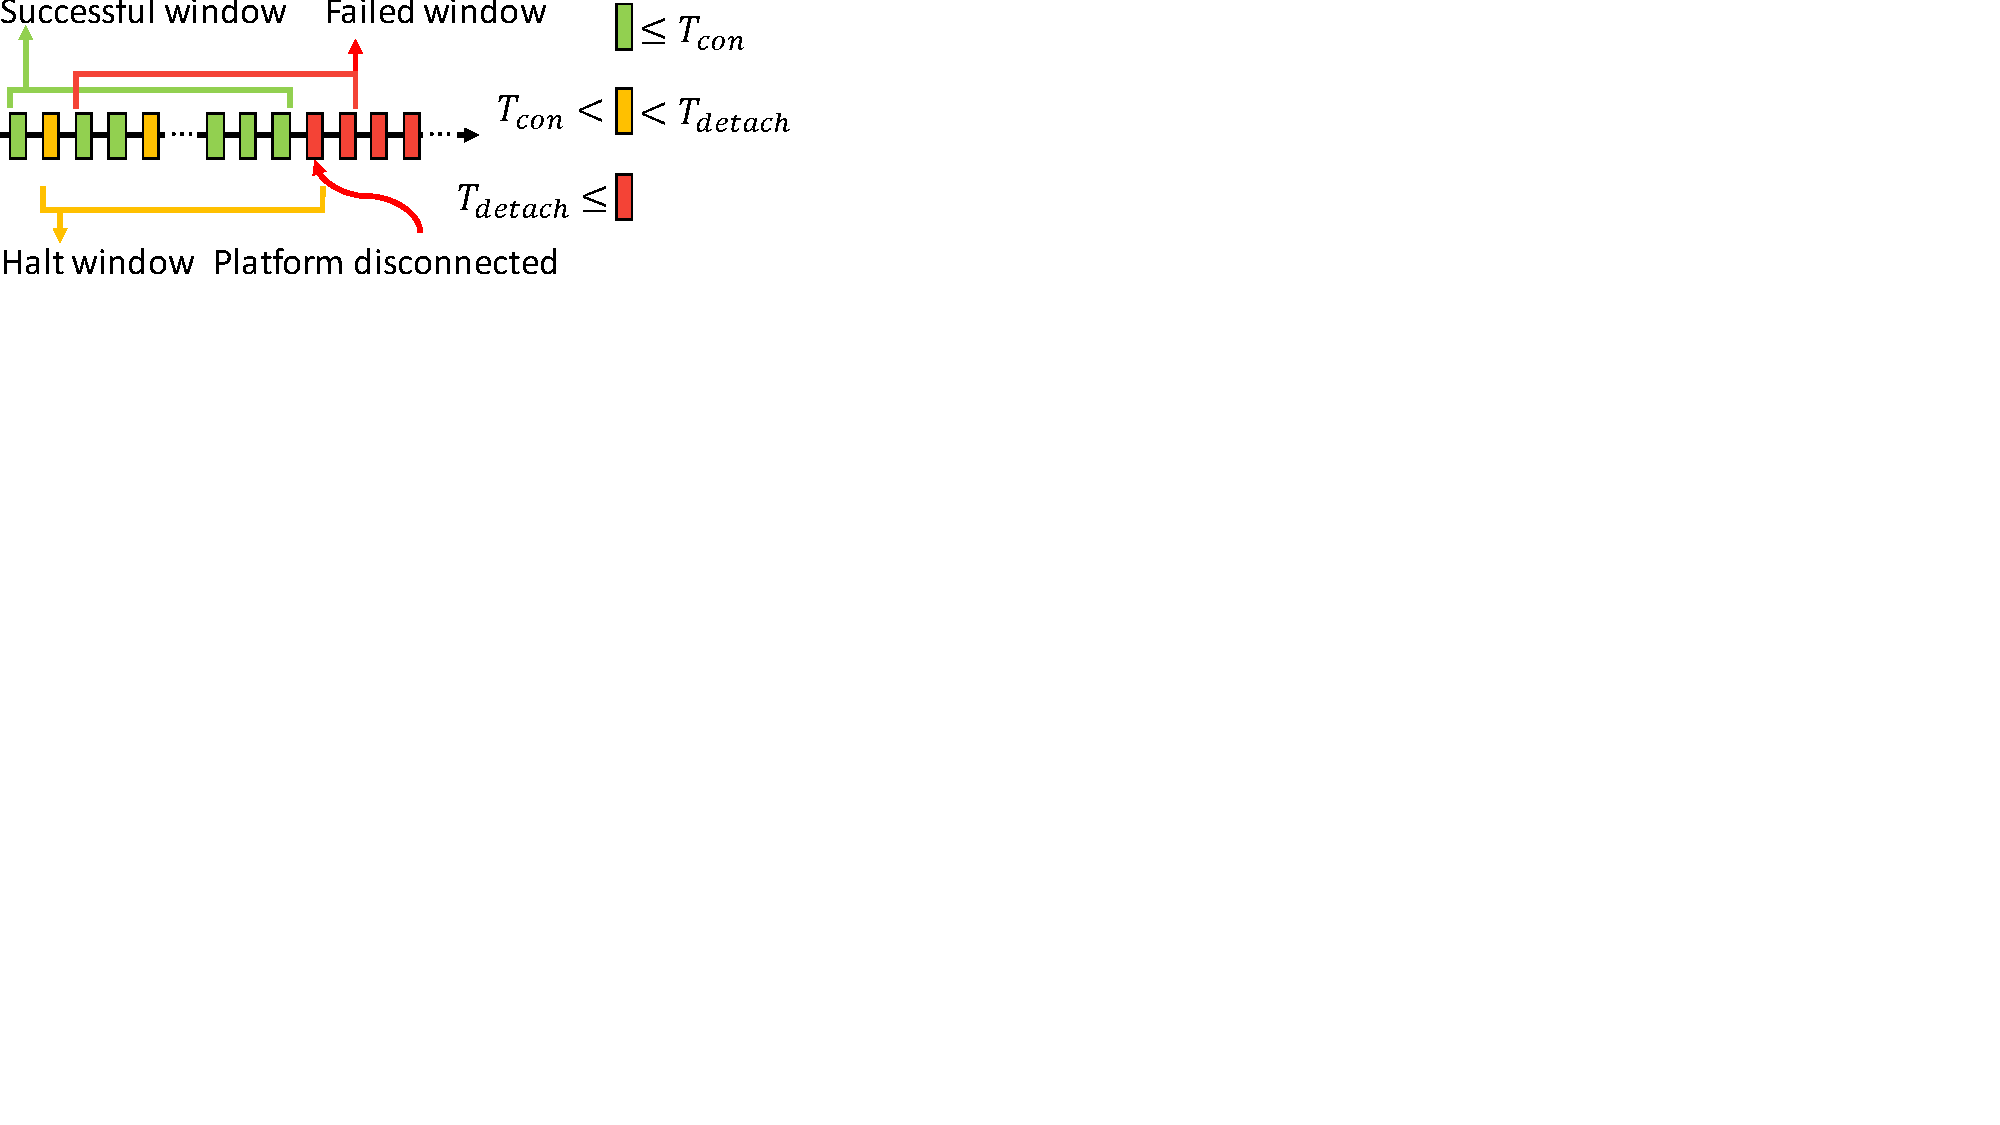
\includegraphics[trim={0 14cm 20cm 0}, clip, width=0.7\linewidth]{chapters/ProximiTEE/figures/SlidingWindow_1.pdf}
   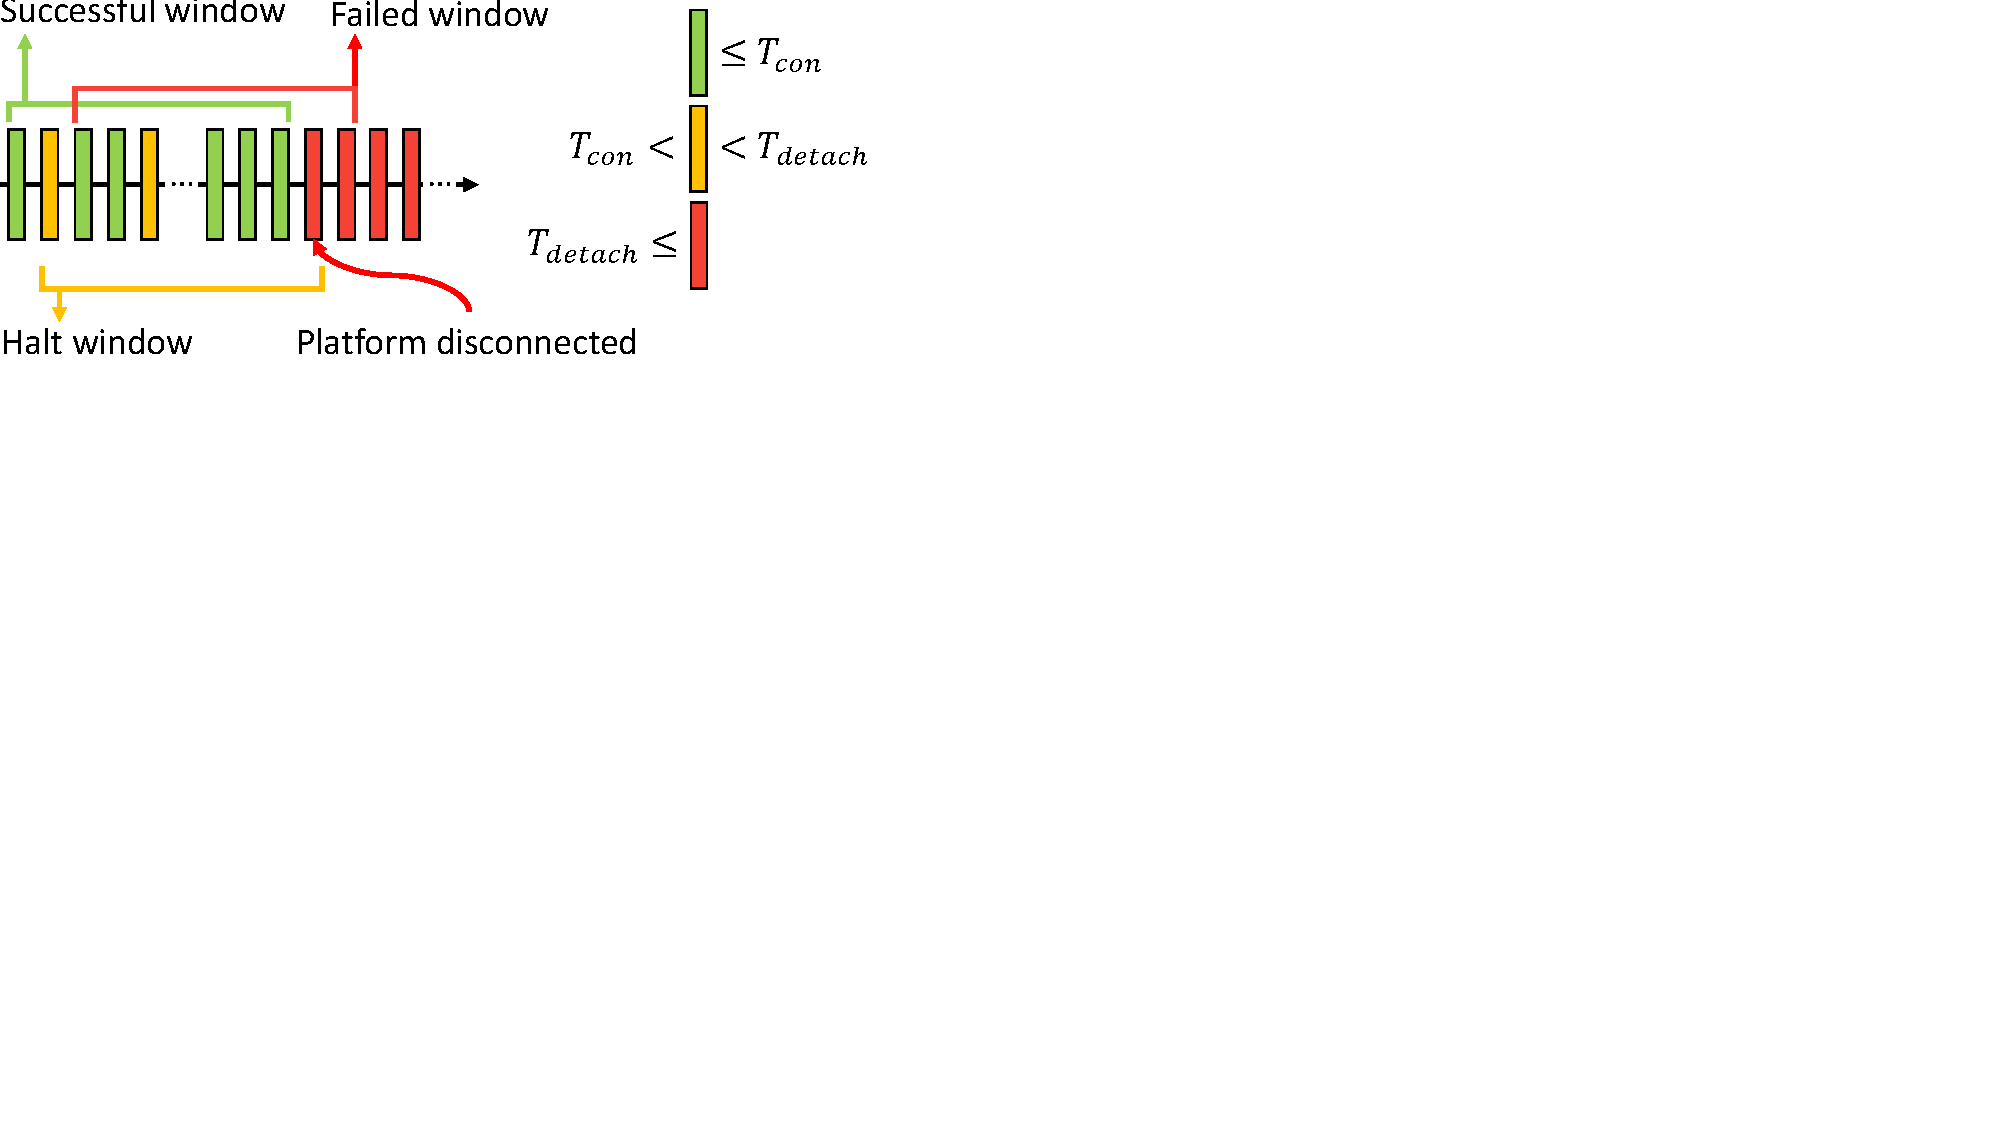
\includegraphics[trim={0 12.5cm 19cm 0}, clip, width=0.7\linewidth]{chapters/ProximiTEE/figures/SlidingWindow.pdf}
    \caption[\name periodic proximity verification]{\textbf{Sliding window} for periodic proximity verification with three different types of challenge-response latencies.}
    \label{fig:slidingWindow}
\end{figure}

As elaborated in Section~\ref{sec:evaluation}, there are three types of latencies in the presence of relay attacks. The first type of response is received faster than the threshold \connect (green in Figure~\ref{fig:slidingWindow}). These responses can only be produced if no attack is taking place. In the second type of response, the latency exceeds \connect, but it is below another, higher threshold \detach (yellow); these are sometimes observed during legitimate connections and sometimes during relay attacks. And third, the latency is equal to or exceeds \detach (red); these latencies are only observed while a relay attack is being performed. Given such a sliding window of periodic challenge-response latencies, we define the following rules for halting or terminating the connection:

\begin{enumerate}
  \item \emph{Successful window: no action.} If at least $k$ responses have latency $\leq$\connect and none of the responses has latency$\geq$\detach, the current window legitimate, and \device keeps the connection active.
 
  \item \emph{Halt window: prevent communication.} If one of the responses has latency $\geq$\detach, we consider the current window a ``halt window,'' and \device stops forwarding data to the enclave until the current window is legitimate again.

  \item \emph{Failed window: terminate channel.} If two or more responses have latencies $\geq$\detach, we consider the current window a ``failed window'', and \device terminates the communication and thus revokes the attested platform.
\end{enumerate} 
\section{Experimental Evaluation}
\label{sec:evaluation}

In order to evaluate the security and reliability of our implementation of \name, we conducted a series of experiments

\subsection{Evaluation Focus: Internet Relay}
\label{sec:evaluation:focus}

For the purposes of our evaluation, we make the distinction between two types of relay attacks. In the first type, the adversary redirects the attestation \emph{over the Internet} to another platform that is under his physical control, and therefore in a \emph{different location}. As we explained in Section~\ref{sec:problemStatement:implication}, such relay attack amplifies the adversary's capabilities the most, as he can now attack the attested enclave using physical side-channels, he has unlimited time to launch digital side-channels, or he can wait for the discovery of new attack vectors. 
 
In the second type of relay attack, the adversary redirects the attestation to another \emph{co-located platform}, like another server on the same server rack. In most cases, attestation relay to a co-located platform does not improve the adversary's chances of attacking the enclave, because typically the adversary has similar control over the co-located platform. The only exception is privilege escalation in cases where the adversary has user privileged on the target platform and system privileges on the co-located platform. 

Next, we focus on demonstrating that an inexpensive \name prototype can be configured to prevent the first (and typically more dangerous) type of relay attacks with very strong security and robustness. Later, in Section~\ref{sec:co-located}, we discuss the second type of relay.


\subsection{Experimental Setup}
\label{sec:evaluation:exp}

To demonstrate that \name prevents relay attacks (over the Internet) we performed two types of experiments. First, we tested the legitimate attestation execution with \name and measured the challenge-response latencies between our prototype and the target platform. Second, we \emph{simulated} a relay attack, where the adversary redirects the attestation to another platform.

\begin{figure}[t]
  \centering
    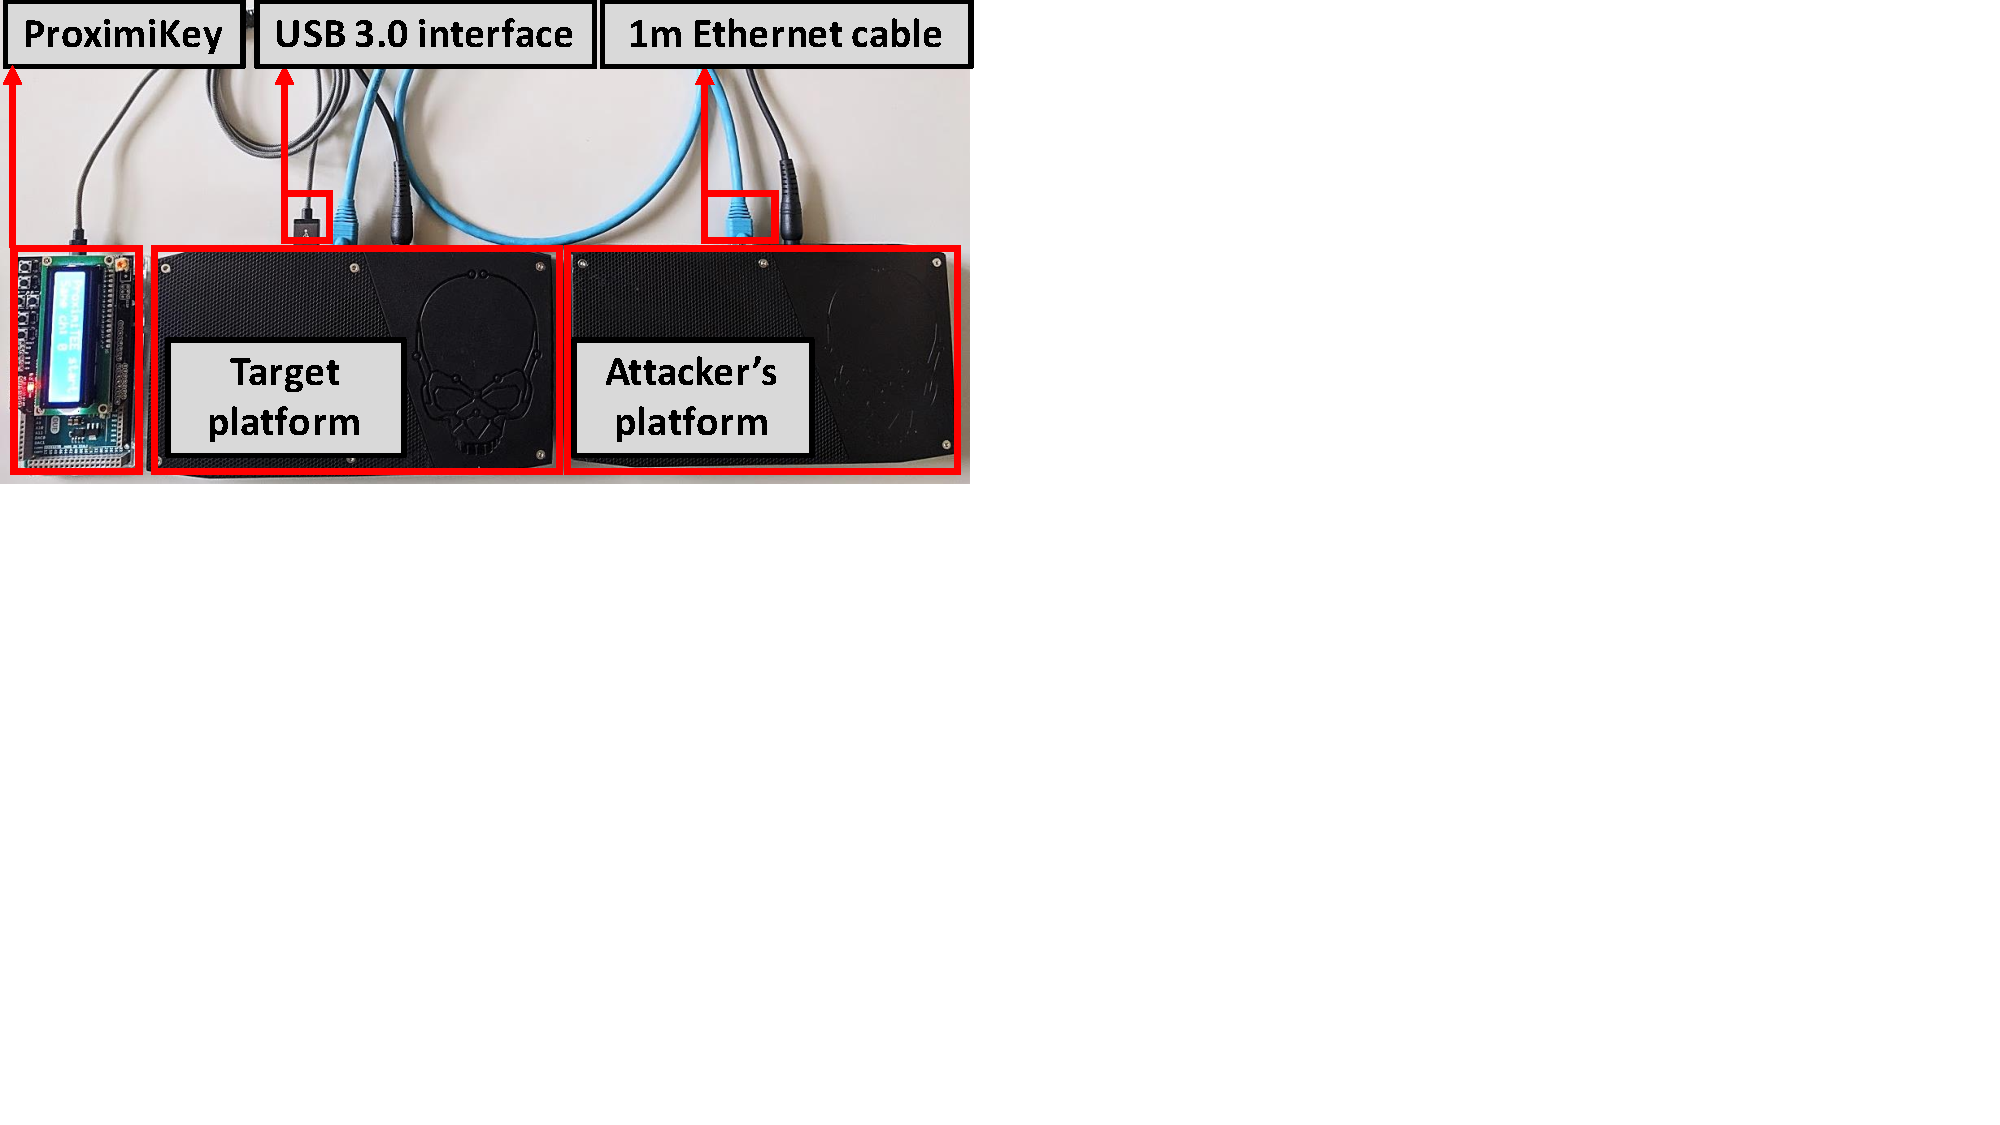
\includegraphics[trim={0 11cm 17cm 0}, clip, width=0.8\linewidth]{chapters/ProximiTEE/figures/Setup2.pdf}
    \caption[\name experimental setup]{\textbf{\name experimental setup} consists of the \device device prototype, the target platform, the attacker's platform and the connection interfaces between them.}

    \label{fig:setup}
\end{figure}

\subsubsection{Assumptions and optimizations.}
To consider the best possible case for the adversary, we made several generous assumptions in his favor, when designing our experimental setup and post-processing of our measurement:

\begin{enumerate}
	\item \emph{Single network hop.} Since we do not want to make any assumptions about the precise network path that the relayed attestation needs to travel, we connected the adversary's platform to the target platform via a direct 1-meter Ethernet cable as seen in Figure~\ref{fig:setup}. With such setup, our goal is to simulate the most direct connectivity and the best possible latency that the adversary could achieve in relay attacks that take place over the Internet. In most realistic attacks, the adversary would need to relay the attestation over multiple network hops which increases the round-trip latency significantly. 

	\item \emph{Instant protocol computation.} Since the adversary might have a faster processor on his platform than the one the one we used in our experiments, we simulated an adversary who is able to perform all computations needed for the proximity verification protocol instantly. Instant replies were simulated by fixing the randomness for the challenges and having precomputed responses for that randomness on the attacker's machine.

	\item \emph{Packet forwarding optimizations.} Since the adversary controls the OS on the target platform, he can perform software-based optimizations to reduce the packet forwarding delay. We experimented with several such optimizations. First, we tested the standard \texttt{ping} tool which gave a latency of around $380\ \mu s$ for one-meter Ethernet connection. After that, we used the \texttt{ping} tool in so called flood mode and measured a reduced average network latency of around $153\ \mu s$ (command \texttt{ping -s 300 -af}). Flood mode achieves faster round-trip time as the it forces the OS to fill up the network queue of the kernel. Based on these measurements, we chose to simulate an attacker that fills the kernel's network queues (on both platforms) similar to the flood mode to minimize latency. We also tested other possible OS-level optimizations, but did not observe material reduction in measured latencies, and thus in our experiments we only use the kernel queue filling.
	
	\item \emph{Infinitely fast network interface.} Since the adversary's platform might have a faster network interface hardware than the one used in our experiments, we chose to simulate an adversary that has infinitely fast network interface. In our experimental setup, both the target platform and the adversary's platform have identical network interfaces. We assume (in the favor of the adversary) that the transmission time spent on the wire is negligible and most the the round-trip latency is due to processing the in the network interface. This allows us to simulate an adversary with infinitely fast network interface by first performing latency measurements and then in a post-processing phase cutting down all the measured latencies by half. Note that the target platform's network interface cannot be replaced by the attacker has he does not have physical access to it.
\end{enumerate}

\subsubsection{Experiments.}
We conducted our experiments on three SGX platforms: two Intel NUC NUC6i7KYK mini-PCs and one Dell Latitude laptop, all equipped with SGX-enabled Skylake core i7 processors and Ubuntu 16.04 LTS installed on them. To measure latencies we used FX-3's GPIO pins that provides 100 nanosecond level accuracy. We performed a total of $20$ million rounds of the protocol for normal attestations and simulated attacks and measured the challenge-response latencies for each. We measure all of them inside the EZ-USB FX3 code. For cross-validation, we tested the \device with the high precision oscilloscope and witnessed identical timing patterns.


\subsection{Latency Distributions}
\label{sec:evaluation:results}



The histogram in Figure~\ref{graph:instatAttackerHisto} on the left represents the challenge-response latencies in the legitimate proximity verification. The histogram on the right shows latencies in a simulated attack (including a post-processing phase where we reduce the adversary's measured network latencies to half to accommodate the assumption of the attacker's infinitely fast network interface).

As can be seen from Figure~\ref{graph:instatAttackerHisto}, the vast majority of the benign challenge-responses take from $145$ to $250 \mu s$ (average is $185 \mu s$, $95\%$ of samples are in between $150\mu s$ and  $200\mu s$). The vast majority of the round-trip times in the simulated attack take from $200$ to $750$ $\mu s$ (average is 264$\mu s$, $95\%$ of samples are in between 209$\mu s$ and 650 $\mu s$). Hence, the average delay of our simulated adversary is only $80 \mu s$. To put this into perspective, even the highly-optimized network connections between major data centers in the same region exhibit latencies from one millisecond upwards~\cite{agarwal_agarwal_2018} which is one order of magnitude more than in our simulated setup.



\begin{figure}[t]
  \centering
    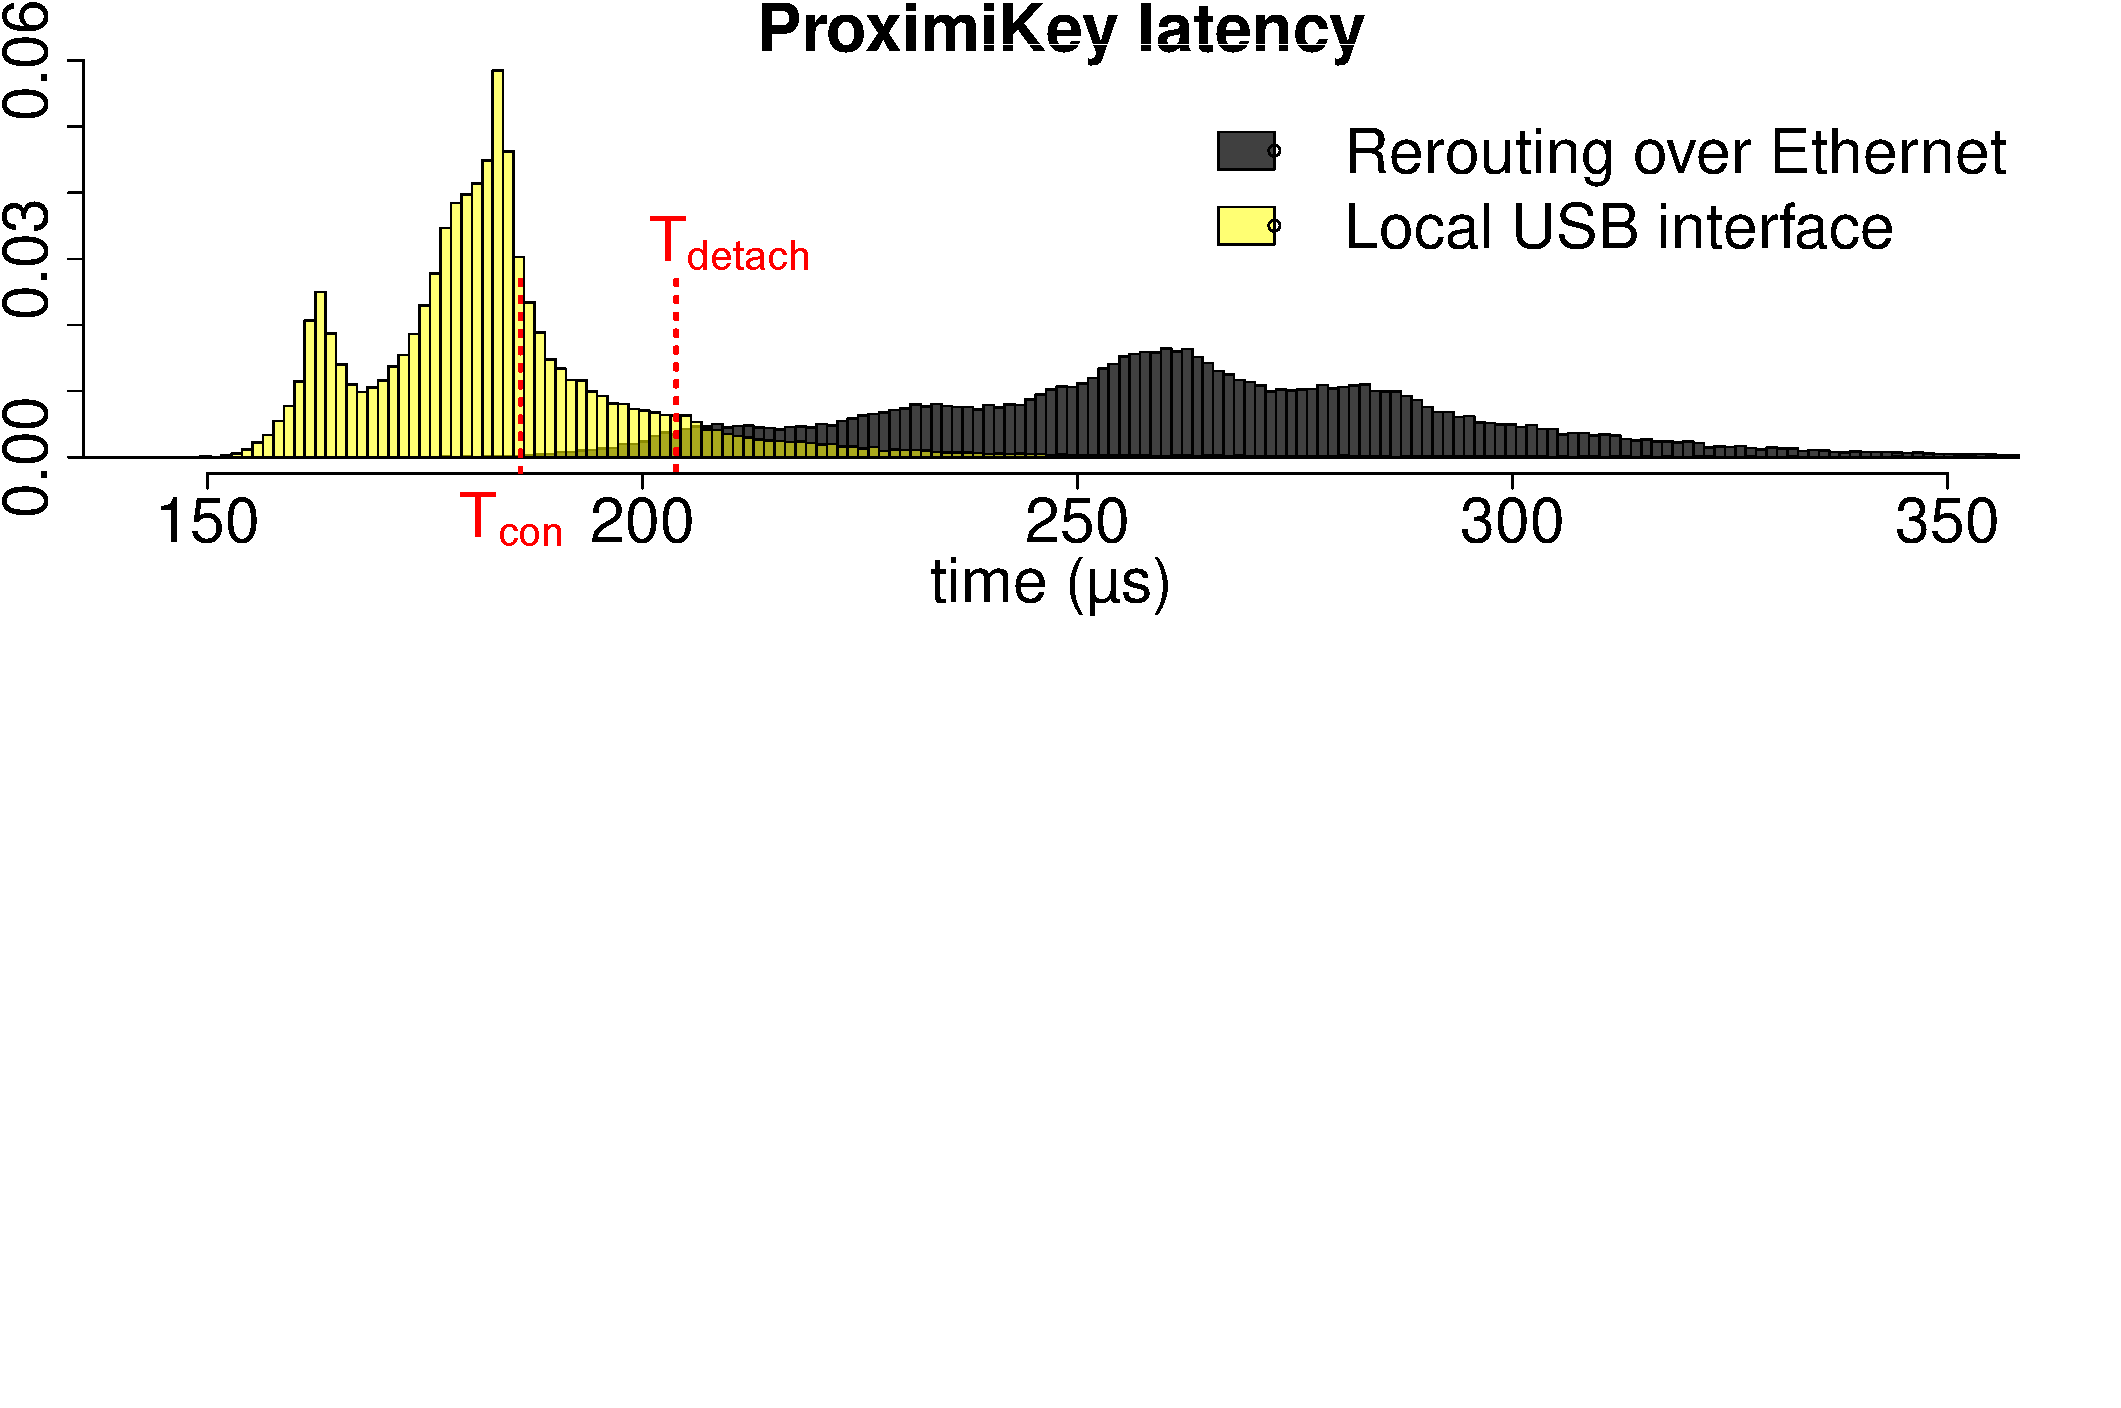
\includegraphics[trim={0 13.4cm 0 0},
    clip,width=\linewidth]{chapters/ProximiTEE/figures/histo.pdf} 
    \caption[Latency distributions]{\textbf{Latency distributions} for legitimate challenge-response rounds (left) and simulated relay attack (right).}
    \label{graph:instatAttackerHisto}
\end{figure}



Besides the latency observed on the side of the embedded device, we measured the time required to compute responses to received challenges on the side of the target platform. We repeated these test on three different SGX platforms and observed results that varied from 6 to 10 $\mu$s. We also measured if the computational load of the target platform influences the time required to compute responses. Under maximum system load (all 8 cores busy), the maximum observed time increased to 20 $\mu$s. Under moderate system load (1 or 2 cores busy), we experience no notable increase in the required computation time. 


\subsection{Initial Proximity Verification Parameters}
\label{sec:evaluation:parameters}

As explained in Section~\ref{sec:systemDesign}, the initial proximity verification is successful when at least fraction $k$ of the $n$ challenge-response latencies are below the threshold \connect.  Now, we explain our strategy for setting these parameters based on the above results.

There are five interlinked parameters that one needs to consider: (i) the legitimate connection latency threshold \connect, (ii) total number of challenge-response rounds $n$, (iii) the fraction $k$, (iv) attacker's success probability $P_{adv}$ that should be negligible, and (v) the legitimate success probability $P_{legit}$ that should be high. We find suitable values for these parameters in the following order:



\newcommand{\mainResultCaption}{\textbf{Distinguishing relay attack.} The attacker's success probability $P_{adv}$ and the legitimate success probability $P_{legit}$ in proximity verification for different number of rounds ($n$) given a fixed $k=0.4$.}


\subsubsection{Finding suitable threshold \connect.} Finding a suitable threshold \connect is a non-trivial task. A very low threshold requires a high number of the challenge-response rounds, since the protocol requires at least a fraction $k$ of the observed responses to be less or equal to \connect and a low threshold has very low cumulative probability value in the latency distribution (see Figure~\ref{fig:cdf}). Conversely, a very high threshold value enables some latencies measured during an attack to be classified as legitimate replies, hence increasing the chances of the attacker to break the proximity verification. To address this challenge, we perform a trial over multiple threshold candidates to evaluate their viability.


Figure~\ref{graph:diffTh} shows the legitimate success probability $P_{legit}$ for different number of rounds ($n\in\{10,20,50,100\}$). We iterate through multiple threshold times (\connect$\in\{183\mu s,184\mu s,185\mu s, 186\mu s, 189\mu s\}$), and $186\mu s$ provides high success ratio for different values of $k$ ($P_{legit}=0.9\{7\}77$ $(n=50)$ and $P_{legit}=0.9\{15\}29\ (n=100)$), where $0.9\{n\}x$ denotes $0.n$-times $9$ followed by $x$.

We test \connect up until $186 \mu s$ because as can be observed in Figure~\ref{graph:instatAttackerHisto} for these values we observe extremely small occurrences ($1.33\times10^{-3}$) of latency responses during an attacking scenario. It is possible to increment the latency further to improve the success probability, but doing so will start increasing the probability for the attacker as well. 
%
After that, we estimate that any latency value less than or equals to the threshold \connect appears with the cumulative probability of $p_{\mathcal{H}} = \Pr[144\leq x \leq 186] = \sum_{i=144}^{186}\Pr[x=i] = 0.693$ (where $144\ \mu s$ is the smallest latency experienced).

The attacker's success probability for a single round is the cumulative probability sampled from the attacker's distribution (the grey histogram in Figure~\ref{graph:instatAttackerHisto}) $p_\mathcal{A} = \Pr[x \leq 186] = \sum_{i=160}^{183}\Pr[x=i] = 1.33 \times 10^{-4}$.


Now, for both cases (simulated attack and benign case) we can model the complete challenge-response protocol of $n$ rounds as a Bernoulli's trial where we look for at least $kn$ responses within $186\ \mu s$ out of $n$. We can write this cumulative probability as a binomial distribution:
%

\begin{align*}
    \Pr[x \geq nk] = \sum_{i=nk}^n\binom{n}{i} (p)^{i}(1-p)^{n-i};~~\text{where}~ p \in \{p_\mathcal{H}, p_\mathcal{A}\}
\end{align*}

\begin{figure}[t]
  \centering
    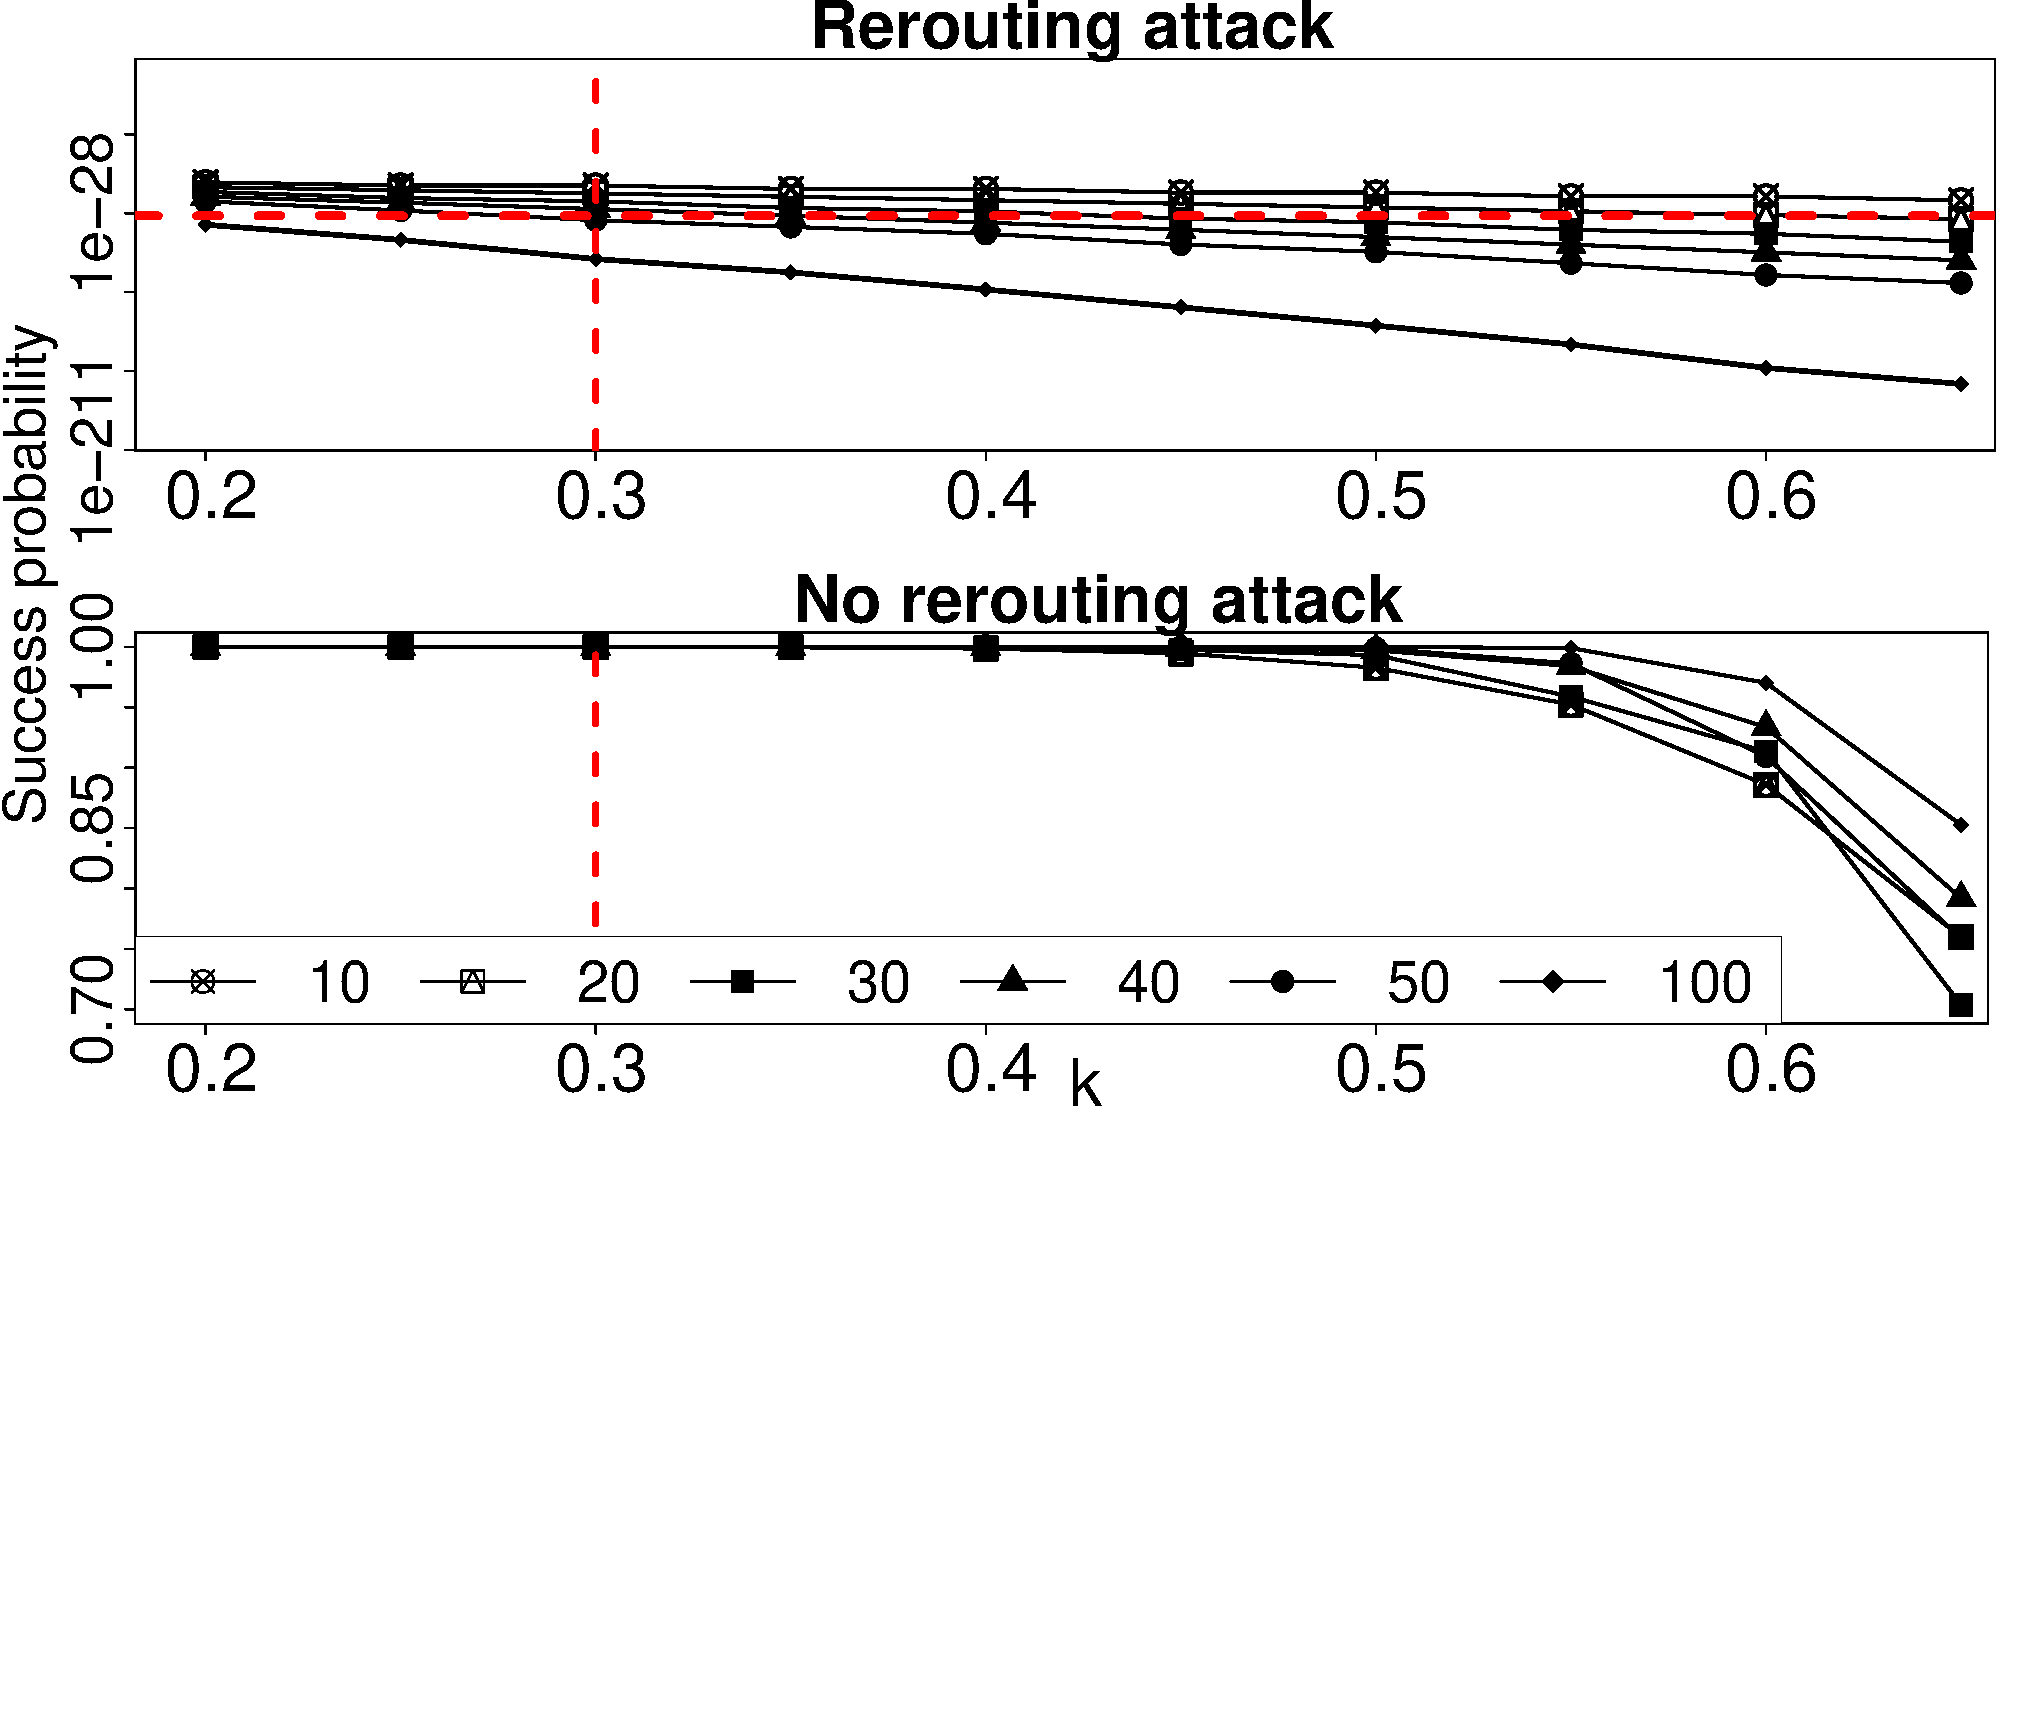
\includegraphics[trim={0 10cm 0 0}, clip, width=\linewidth]{chapters/ProximiTEE/data/fx3_data/round_comp_new.pdf}
    \caption[Finding suitable fraction $k$]{\textbf{Finding suitable fraction $k$.} The graph shows the legitimate enclave's success probability in an ideal scenario and the attacker's success probability in rerouting attack scenario with varying $k$.}
    \label{graph:roundSuccess}
\end{figure}



\begin{figure}[h]
  \centering
    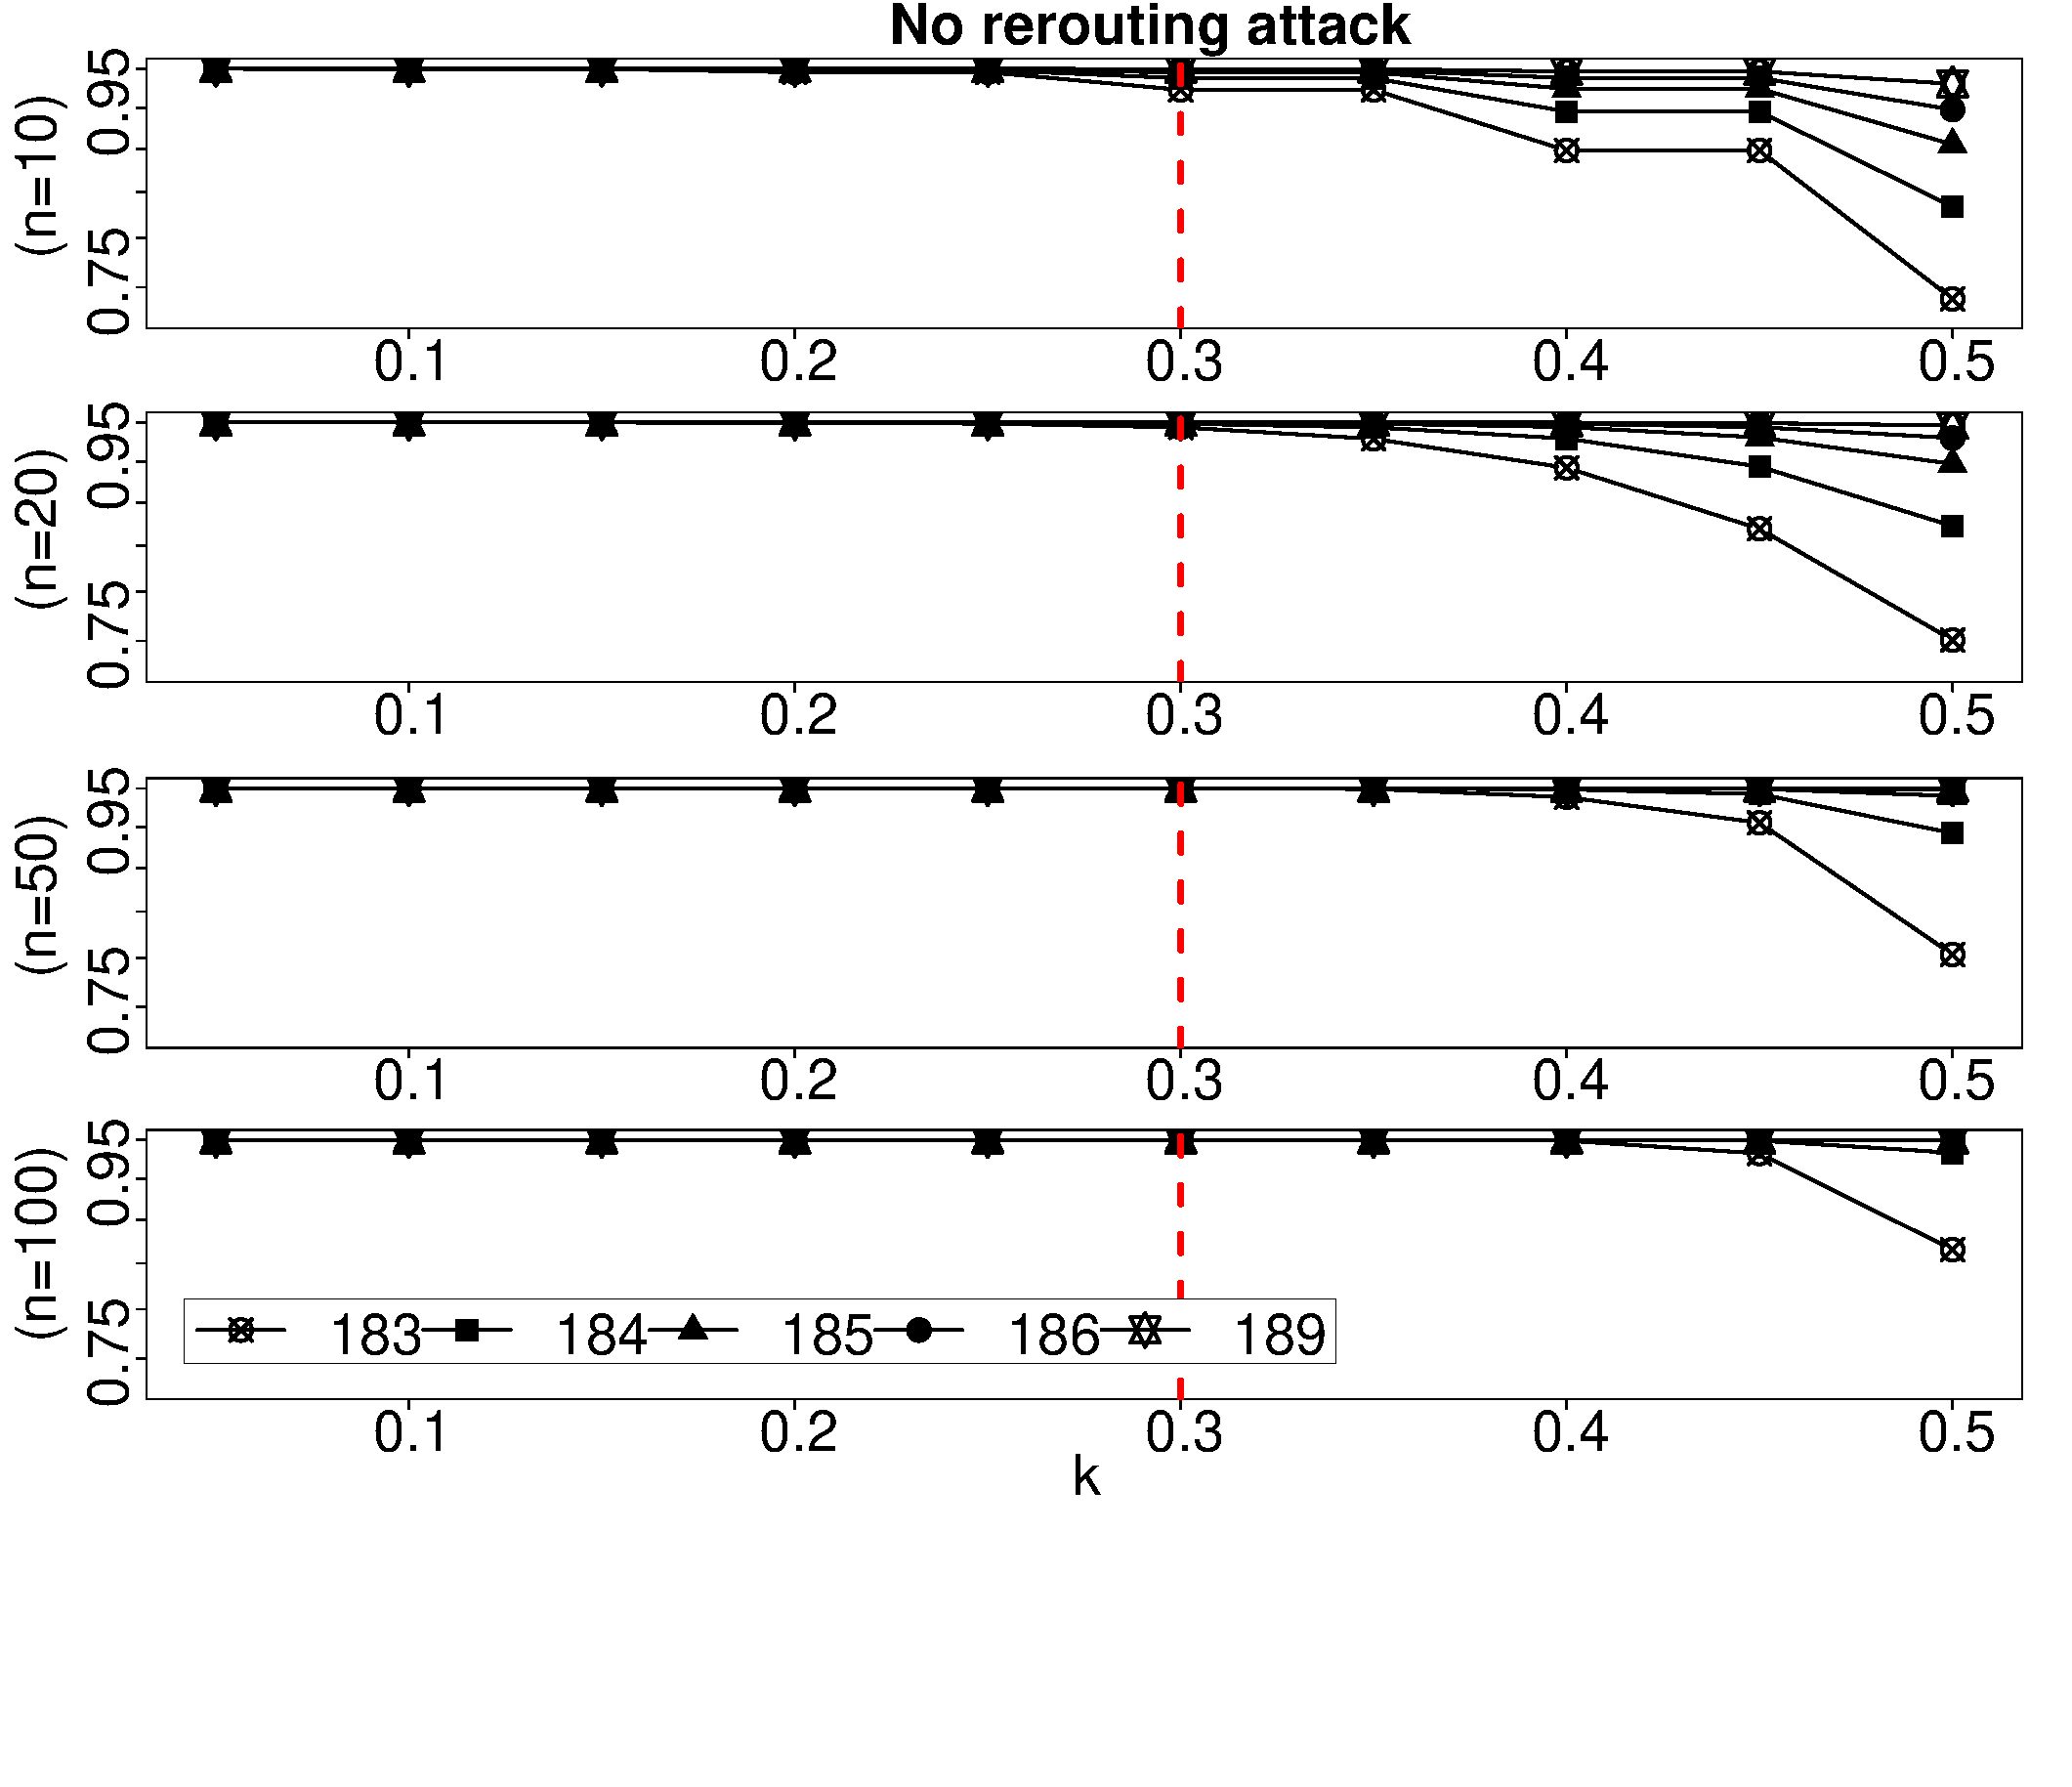
\includegraphics[trim={0 5cm 0 0}, clip, width=\linewidth]{chapters/ProximiTEE/data/fx3_data/timeRound.pdf}
    \caption[Legitimate attestation success probability for different \connect values]{\textbf{Legitimate attestation success probability for different \connect values.} The chosen value \connect $=186\ \mu s$ gives success probability $0.999999977$ for number of trials at least 15 out of $n=50$ rounds when $k=0.3$.}
    \label{graph:diffTh}
\end{figure}


\begin{figure}[h]
  \centering

    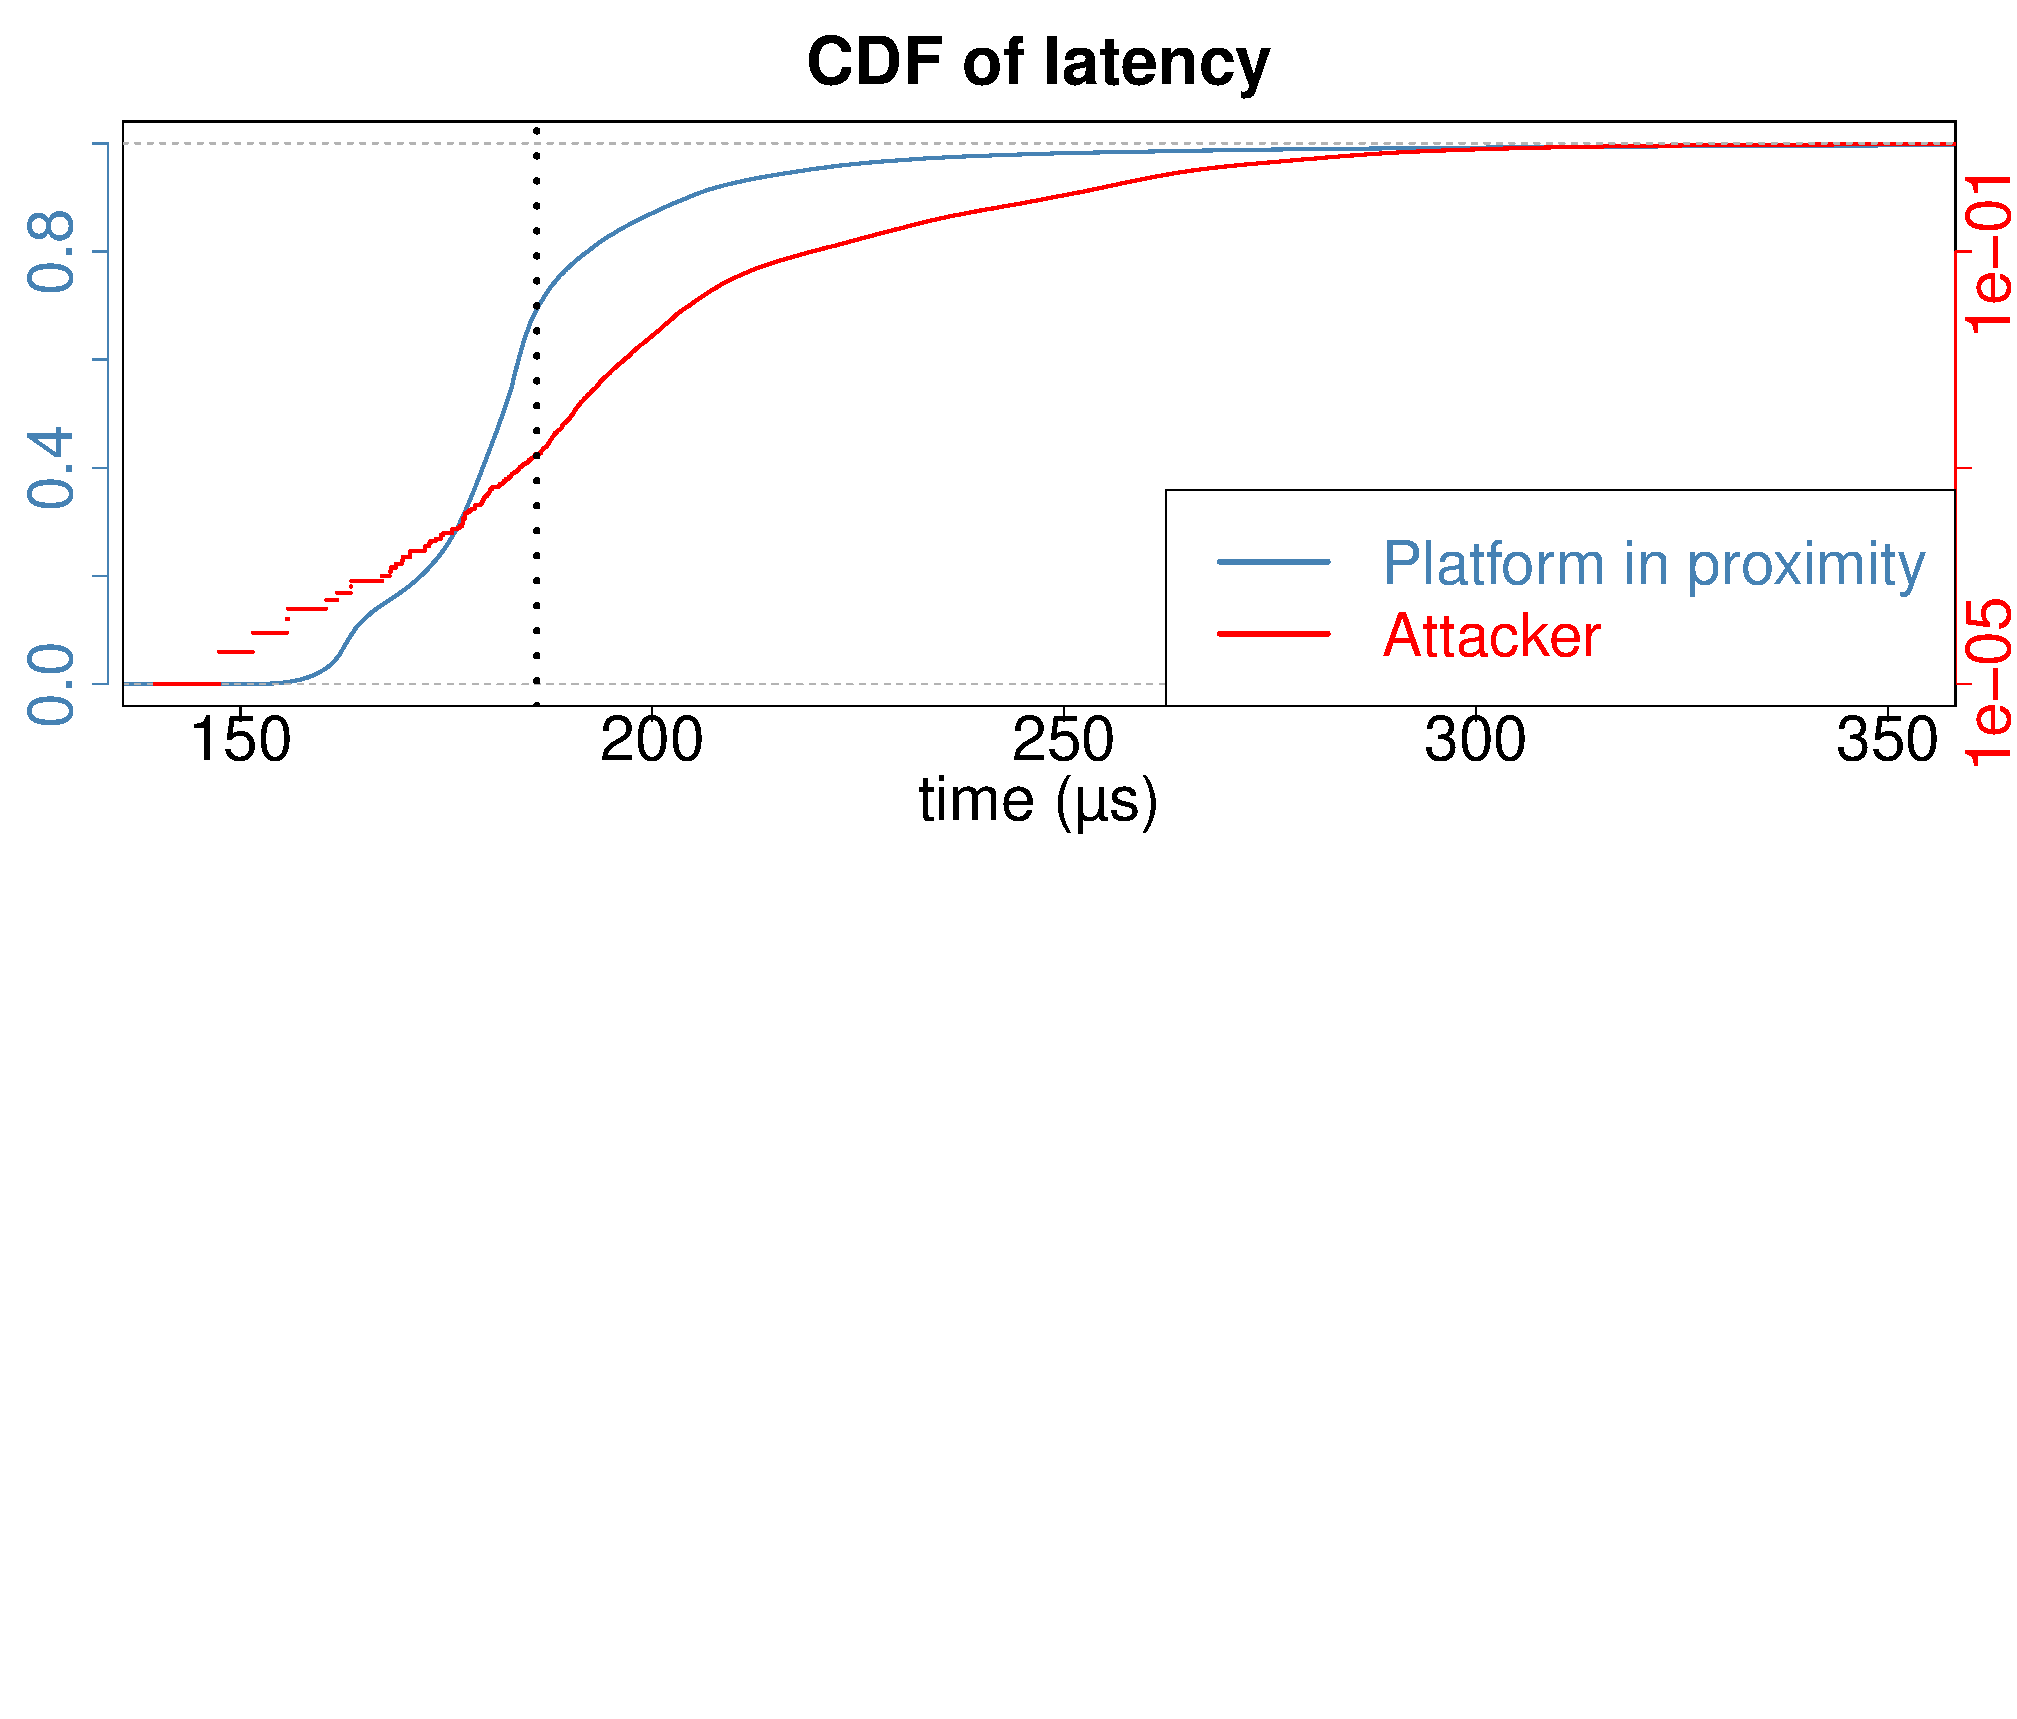
\includegraphics[trim={0 15cm 0 0}, clip, width=0.9\linewidth]{chapters/ProximiTEE/data/fx3_data/CDF_N.pdf}
    \caption[Cumulative distribution function for latencies]{\textbf{Cumulative distribution function for latencies.} We set the threshold \connect at 183 $\mu s$ which has a cumulative probability of $0.693$ in the experiment where no rerouting attack takes place with probability of $1.33\times10^{-4}$.}
    \label{fig:cdf}
\end{figure}


\subsubsection{Choosing a suitable fraction $k$.} The next step of the evaluation is to find a suitable fraction $k$ based on the threshold time \connect. Note that both the success probability of the attacker and the legitimate enclave is calculated as the cumulative probability from a binomial distribution (from $nk$ to $n$). Hence, we require to choose a suitable value of $k$ that maximizes $P_{legit}$ while minimizing $P_{adv}$.

We calculate two graphs that are depicted in Figure~\ref{graph:roundSuccess} where the x-axis denotes $k$, and the y-axis denotes attacker's success probability $P_{adv}$ and legitimate success probability $P_{legit}$, respectively, while using \connect$=186 \mu s$. We observe a sharp decrease in the legitimate success probability at $k=0.3$. Hence, fix $k=0.3$ to achieve the maximum $P_{legit}$. Additionally, in the graph of attacker's success probability, the red horizontal line is placed at $10^{-30} \approx 2^{-100}$. Hence we propose to choose any round configuration bellow this horizontal line, where $n \geq 40$. With number of rounds set to $n=50$ and $k=0.3$, we have $P_{legit}=0.99999997$ and $P_{adv}=3.55\times 10^{-34}$. Similar result could be also observed in Figure~\ref{graph:roundSuccess} where the success probability of the legitimate enclave decreases significantly after $k=0.55$ for \connect$=186\mu s$.



\subsubsection{Generalizing the number of rounds $n$.} Figure~\ref{graph:instatAttackerHisto} extends this analysis to the general number of challenge-response rounds spanning from $n=2$ to $100$. Here we compute the probability of attacker returning the reply within $186 \mu s$ for at least $k=0.3$ fraction of challenges. The y-axis denotes the attacker's success probability which diminishes overwhelmingly with the increasing number of challenges (keeping the fraction constant at $k=0.3$). 



\begin{figure}[h]
  \centering
    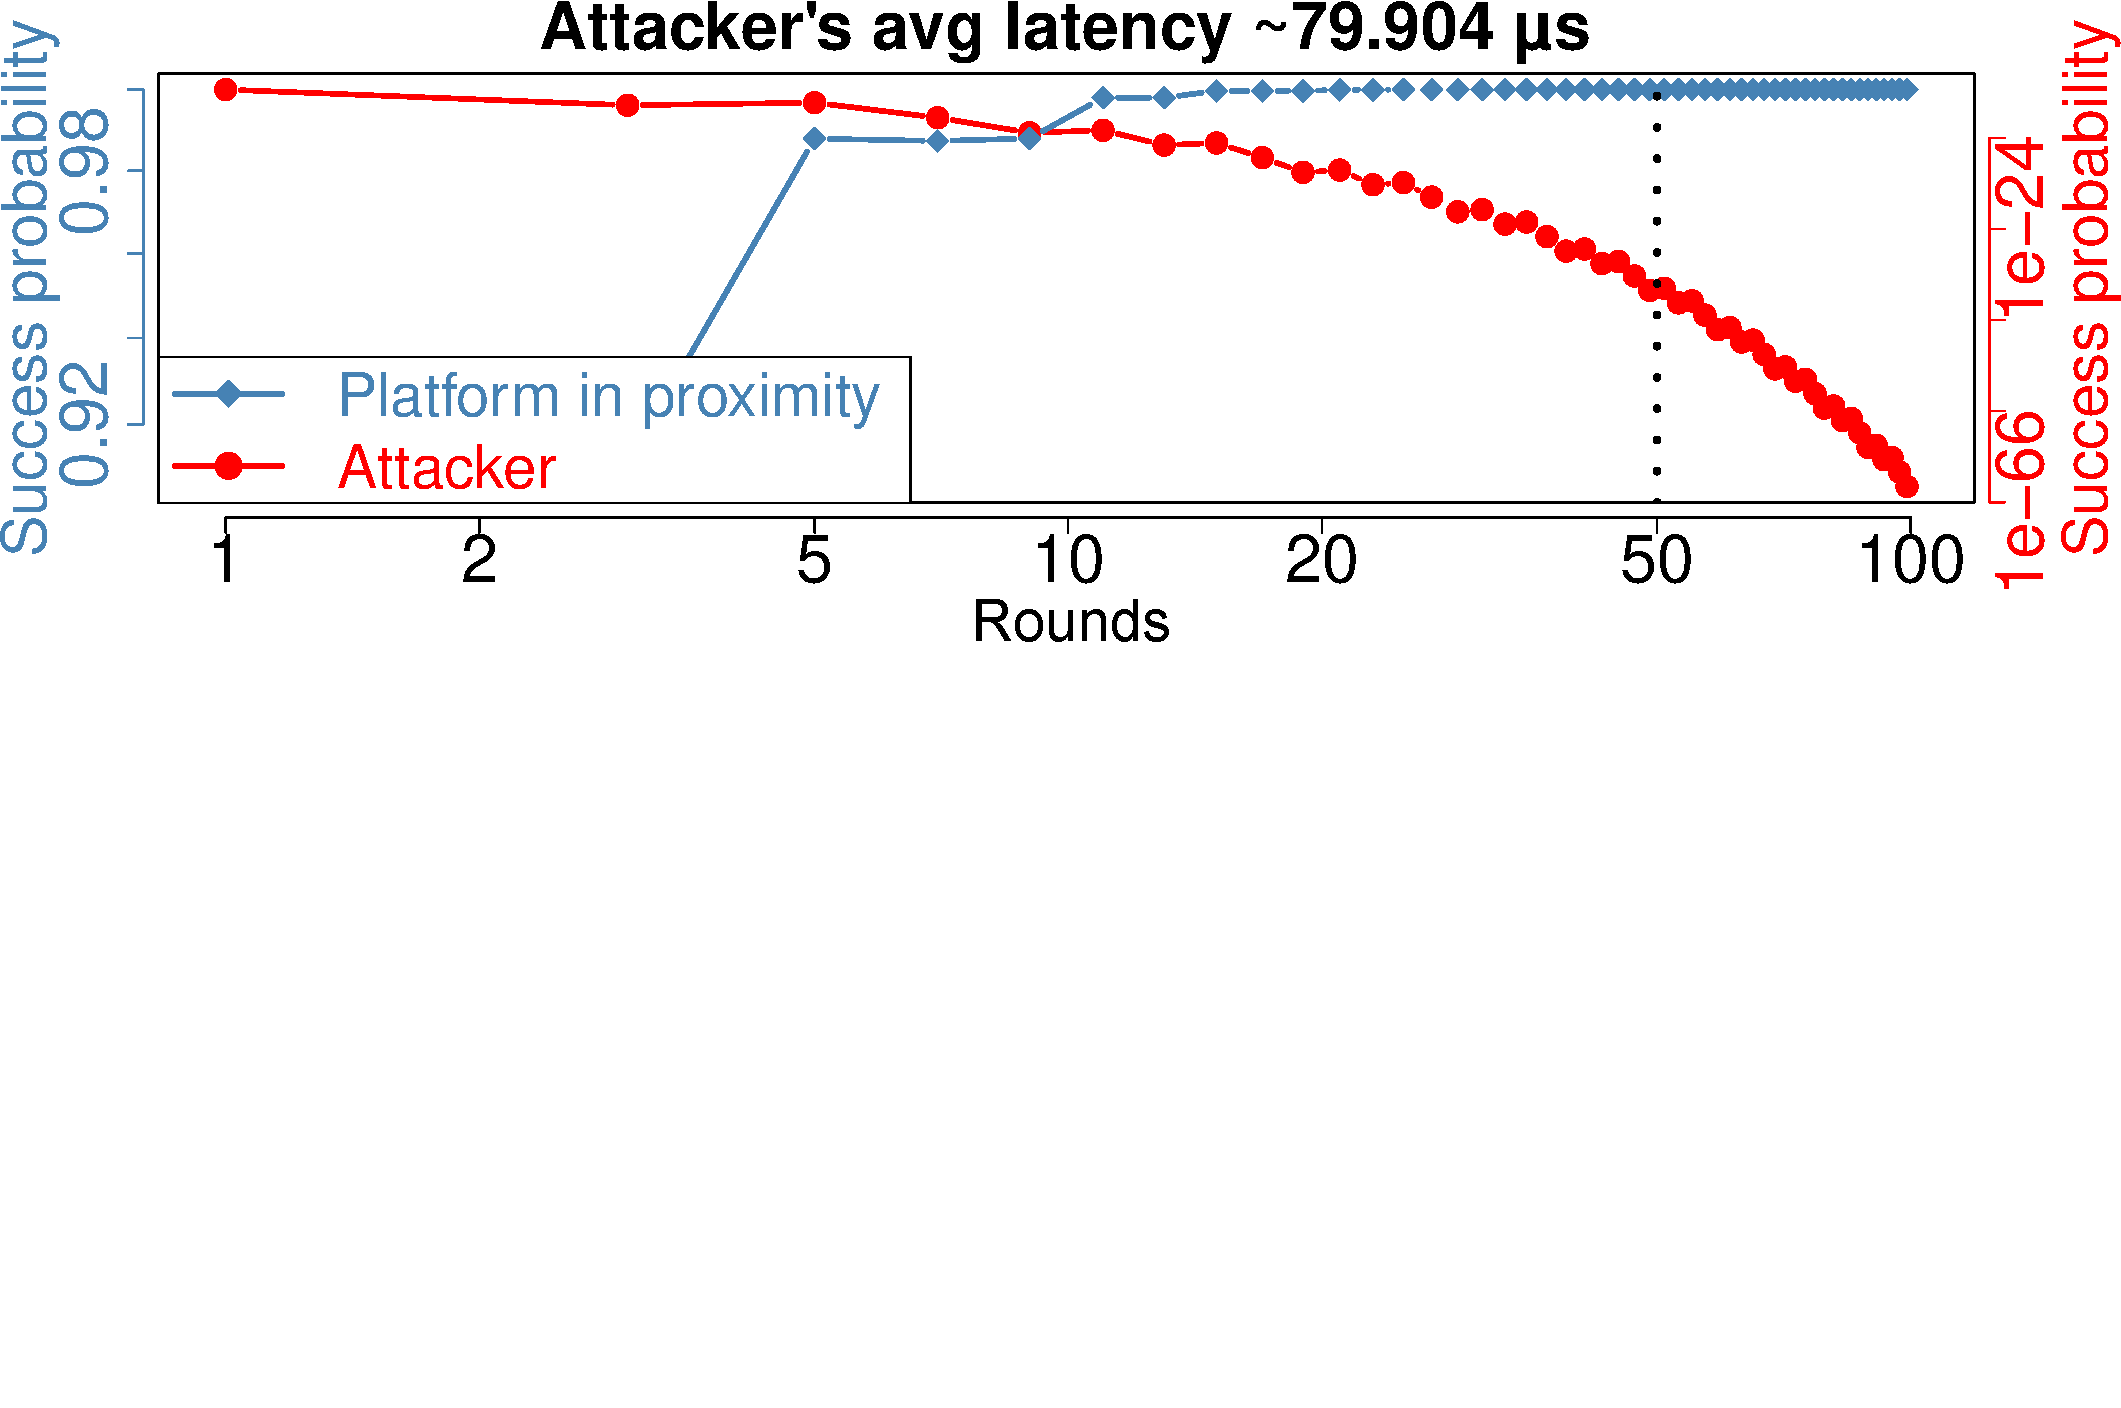
\includegraphics[trim={0 12.8cm 0 0}, clip, width=0.9\linewidth]{chapters/ProximiTEE/figures/InstantAttackerSuccess.pdf}
    \caption[\name distinguishing relay attack]{\textbf{\name distinguishing relay attack.} The figure shows the attacker's success probability $P_{adv}$ and the legitimate success probability $P_{legit}$ for different number of rounds $n$ given a fixed $k$.}

    \label{graph:instantAttackerSuccess}
\end{figure}


\subsubsection{Main result.} Figure~\ref{graph:instantAttackerSuccess} shows the legitimate enclave's success probability $P_{legit}$ and the attacker's success probability $P_{adv}$ with different number of rounds. Based on our experiments we set \connect= 186$\mu s$ (see Figure~\ref{graph:instatAttackerHisto}), the threshold fraction $k=0.3$ and the number of rounds $n=50$ which yields a very high legitimate success probability $P_{legit}=0.999999977$ and a negligible attacker's success probability $P_{adv}=3.55\times 10^{-34}$.





\subsection{Periodic Proximity Verification Parameters}
\label{sec:evaluationL:continuousParameters}


For periodic proximity verification we have two main requirements. First, the attacker's success probability $P'_{adv}$ must be negligible. Recall that $P'_{adv}$ refers to an event where the device is detached but the connection is not terminated sufficiently fast. Second, the probability of false positives $P'_{fp}$ should be very low. $P'_{fp}$ refers to an event where the connection is terminated when the device is still attached. Next, we explain the three-step process to set up parameters \detach, $w$ and $f$ for the periodic proximity verification:

\begin{enumerate}
  \item We find out a suitable latency \detach that define the yellow or red round in Figure~\ref{fig:slidingWindow}. The yellow window defines the round of challenge response latency between \connect and \detach, while the red window defines a latency more than \detach. Hence, the probabilities $\Pr[T_{con}\leq \mathcal{L}_{legit}\leq T_{detach}]=\Pr[legit\in\text{yellow}]$, and $\Pr[\mathcal{L}_{legit} \geq T_{detach}]=\Pr[legit\in\text{red}]$ should be very low. $\mathcal{L}_{legit}$ and $\mathcal{L}_{A}$ denote the latency of the legitimate enclave running on the platform in proximity and remote attacker platform's latency respectively.
  \item Based on the threshold \detach, we select a suitable sliding window size $w$ to minimize the attacker success probability $P'_{adv}$ to a negligible quantity.
  \item We fix a suitable frequency $f$ for the periodic challenges. A high $f$ value terminate the communication very fast, leaving very small attacking window.
\end{enumerate}

\subsubsection{Finding suitable threshold \detach.} We set the threshold \detach to $510\ \mu s$. We choose this value as we experience zero sample from the timing distribution (refer to the `yellow' distribution Figure~\ref{graph:instatAttackerHisto}) where no rerouting attack takes place. While in the attacker's distribution, the cumulative probability of the response occurring between \connect and \detach is $Pr[$\connect$\leq \mathcal{L}_{A} \leq$\detach$]=\sum_{i=451}^{510}\Pr[\mathcal{L}_{A}=i]=1.4\times10^{-2}$. 
%We account for the experimental error in our model using the standard error of the mean as  $p_e \approx 1.06\times10^{-4}$. The value $p_e$ signifies that a legitimate enclave running on the platform in proximity may take more than 649 $\mu s$ to respond. 
Using \detach, we can now define the challenge response rounds in Figure~\ref{fig:slidingWindow} for a \emph{single round} as following:

\begin{align*}
\Pr[\mathcal{L}_{legit}\leq T_{con}]&=\Pr[legit\in\text{green}]=0.75\\
\Pr[T_{con}< \mathcal{L}_{legit}< T_{detach}]&=\Pr[legit\in\text{yellow}]= 0.237\\
\Pr[\mathcal{L}_{legit}\geq T_{detach}]&=\Pr[legit\in\text{red}]= 7.09\times10^{-3}\\
\Pr[\mathcal{L}_{A}\leq T_{con}]&=\Pr[A\in\text{green}]=9.73\times10^{-5}\\
\Pr[T_{con}< \mathcal{L}_{A}< T_{detach}]&=\Pr[A\in\text{yellow}]= 1.4\times10^{-2}\\
\Pr[\mathcal{L}_{A}\geq T_{detach}]&=\Pr[A\in\text{red}]= 0.985\\
\end{align*} 


\subsubsection{Finding suitable sliding window size $w$.} Sliding window size is analogous to that of the number of rounds $n$. We keep  the size of the sliding window as $w=n=50$ as it only requires the \device to remember the past $50$ interactions and achieve high probability for the legitimate enclave and negligible success probability for the attacker. Similar to the previous approach, only if $20$ out of $50$ ($k=0.4$) challenge-response round where responses are within $470\ \mu s$, \name yields success probabilities as the following:

\begin{align*}
 \Pr[A \in \text{success window}]&=P'_{adv} = P'_{fn}= 2.71\times 10^{-67}\\
 \Pr[A \in \text{failed window}]&=\Pr[A\in\text{red}]^2=0.970\\
 \Pr[legit \in \text{success window}]&=0.999999965\\
 \Pr[legit \in \text{failed window}]&=P'_{fp}=\Pr[legit\in\text{red}]^2=5\times10^{-5}
\end{align*}

The probability that a halt window event occurs for a legitimate \app running on the platform in proximity is $\Pr[legit\in\text{red}]\approx 7.09\times10^{-3}$. The \device halts all the data communication to the target platform until the next periodic proximity verification.

If two or more than two latencies $\geq 510\mu s$ (\detach) are received, the \device terminates the connection and revoke the platform. The downtime that can happen as a result of false positive during a connection of 10 years is around $2$ minutes.

\subsubsection{Finding suitable frequency $f$.} The frequency $f$ determines how fast the connection is terminated in case the \device device is detached. Note that the \device takes around $12$ $ms$ on average to issue a new random challenge (by reading out the noise of the analog pins of the Arduino board) in the legitimate case. Hence, by performing a round of the protocol as soon as the previous is over, we achieve the maximum attainable average frequency of $\sim83$ rounds per second. We use this frequency as it consumes only $6.48$ KB (0.0011\% of the 
channel capacity) and allows the communication channel to be halted on average after $12 ms$ of the start of a relay attack and terminated in $24 ms$.

\subsubsection{Summarizing the result of \name periodic verification} 
Based on the above strategy, we set the periodic proximity verification parameters as follows: $\Pr[A \in \text{success window}]=P'_{adv} = P'_{fn}= 3.55\times 10^{-34}$, $\Pr[legit \in \text{success window}]=0.999999977$ and $\Pr[legit \in \text{failed window}]=P'_{fp}=\Pr[legit\in\text{red}]^2=1.6\times10^{-4}$ and \detach = $205 \mu s$ (see Figure~\ref{graph:instatAttackerHisto}). If at least two latencies above \detach are received, the \device terminates the connection and revokes the platform. The average downtime due to false positives occurring during a connection of 10 years is around $2$ minutes. 




\subsection{Performance Analysis}

In addition, we evaluated the following two performance metrics:

\begin{enumerate}
  \item \emph{Start-up latency.} The initial proximity verification takes $2$ ms. The complete connection establishment including attestation and \tls handshake takes less than 1 second.  
  


  \item \emph{Operational latency and data overhead.} Our solution adds around $200 \mu s$ of additional latency for \tls and transport over the native \usb interface of the FX3. The data overhead is around 80 bytes per packet for the header and the MAC. Execution of the periodic \name protocol with $83$ rounds/second requires around $156.14$ KBytes/s of data which is only $2.4 \times 10^{-3}$\% of the \usb 3.0 channel capacity. 


\end{enumerate}


\subsection{Additional Experimental Results}


\begin{figure}[t]
  \centering
    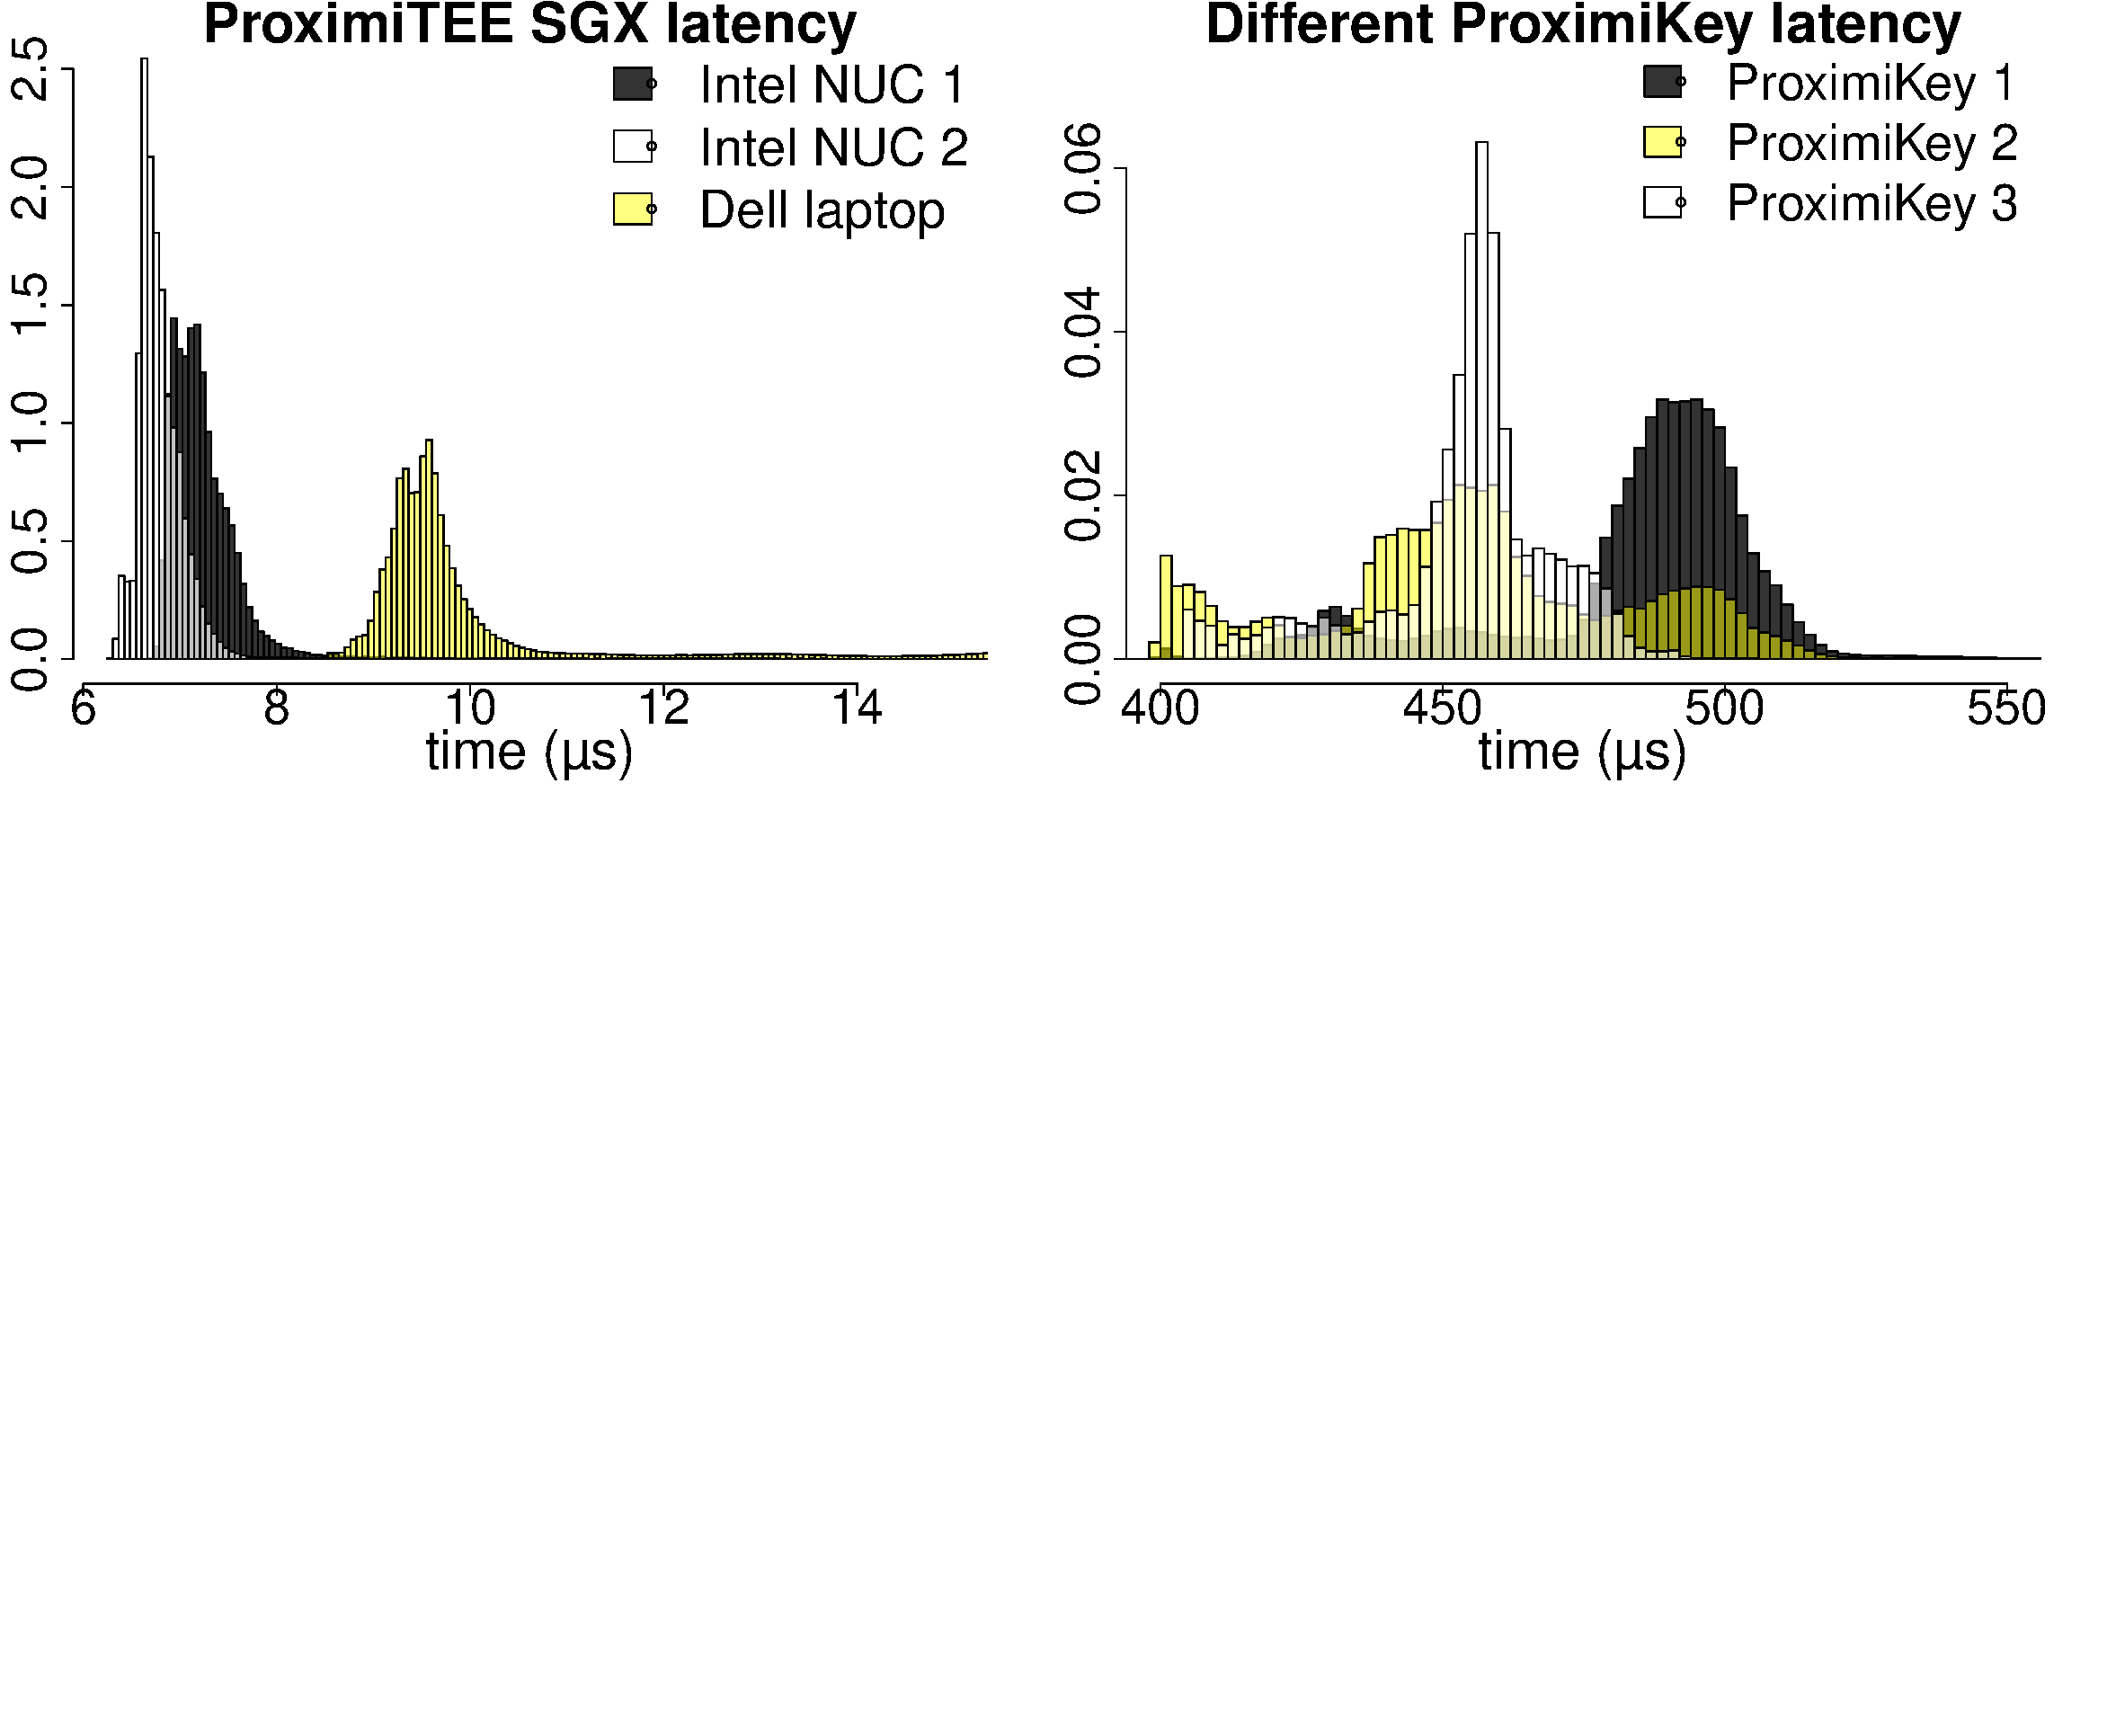
\includegraphics[trim={0 18cm 0 0}, clip, width=\linewidth]{chapters/ProximiTEE/data/graph/PlatformDevice_1.pdf}
    \caption[Effect of different target platforms/\device on the latency.]{\textbf{Effect of different target platforms/\device on the latency.} We evaluates latencies using three different SGX platforms. The Intel NUCs were few microseconds faster. Additionally, we evaluated latencies using three different FX3 boards. The latencies are consistent.}
    %\vspace{-17pt}
    \label{graph:sgxLatency}
\end{figure}

\begin{figure}[t]
  \centering
    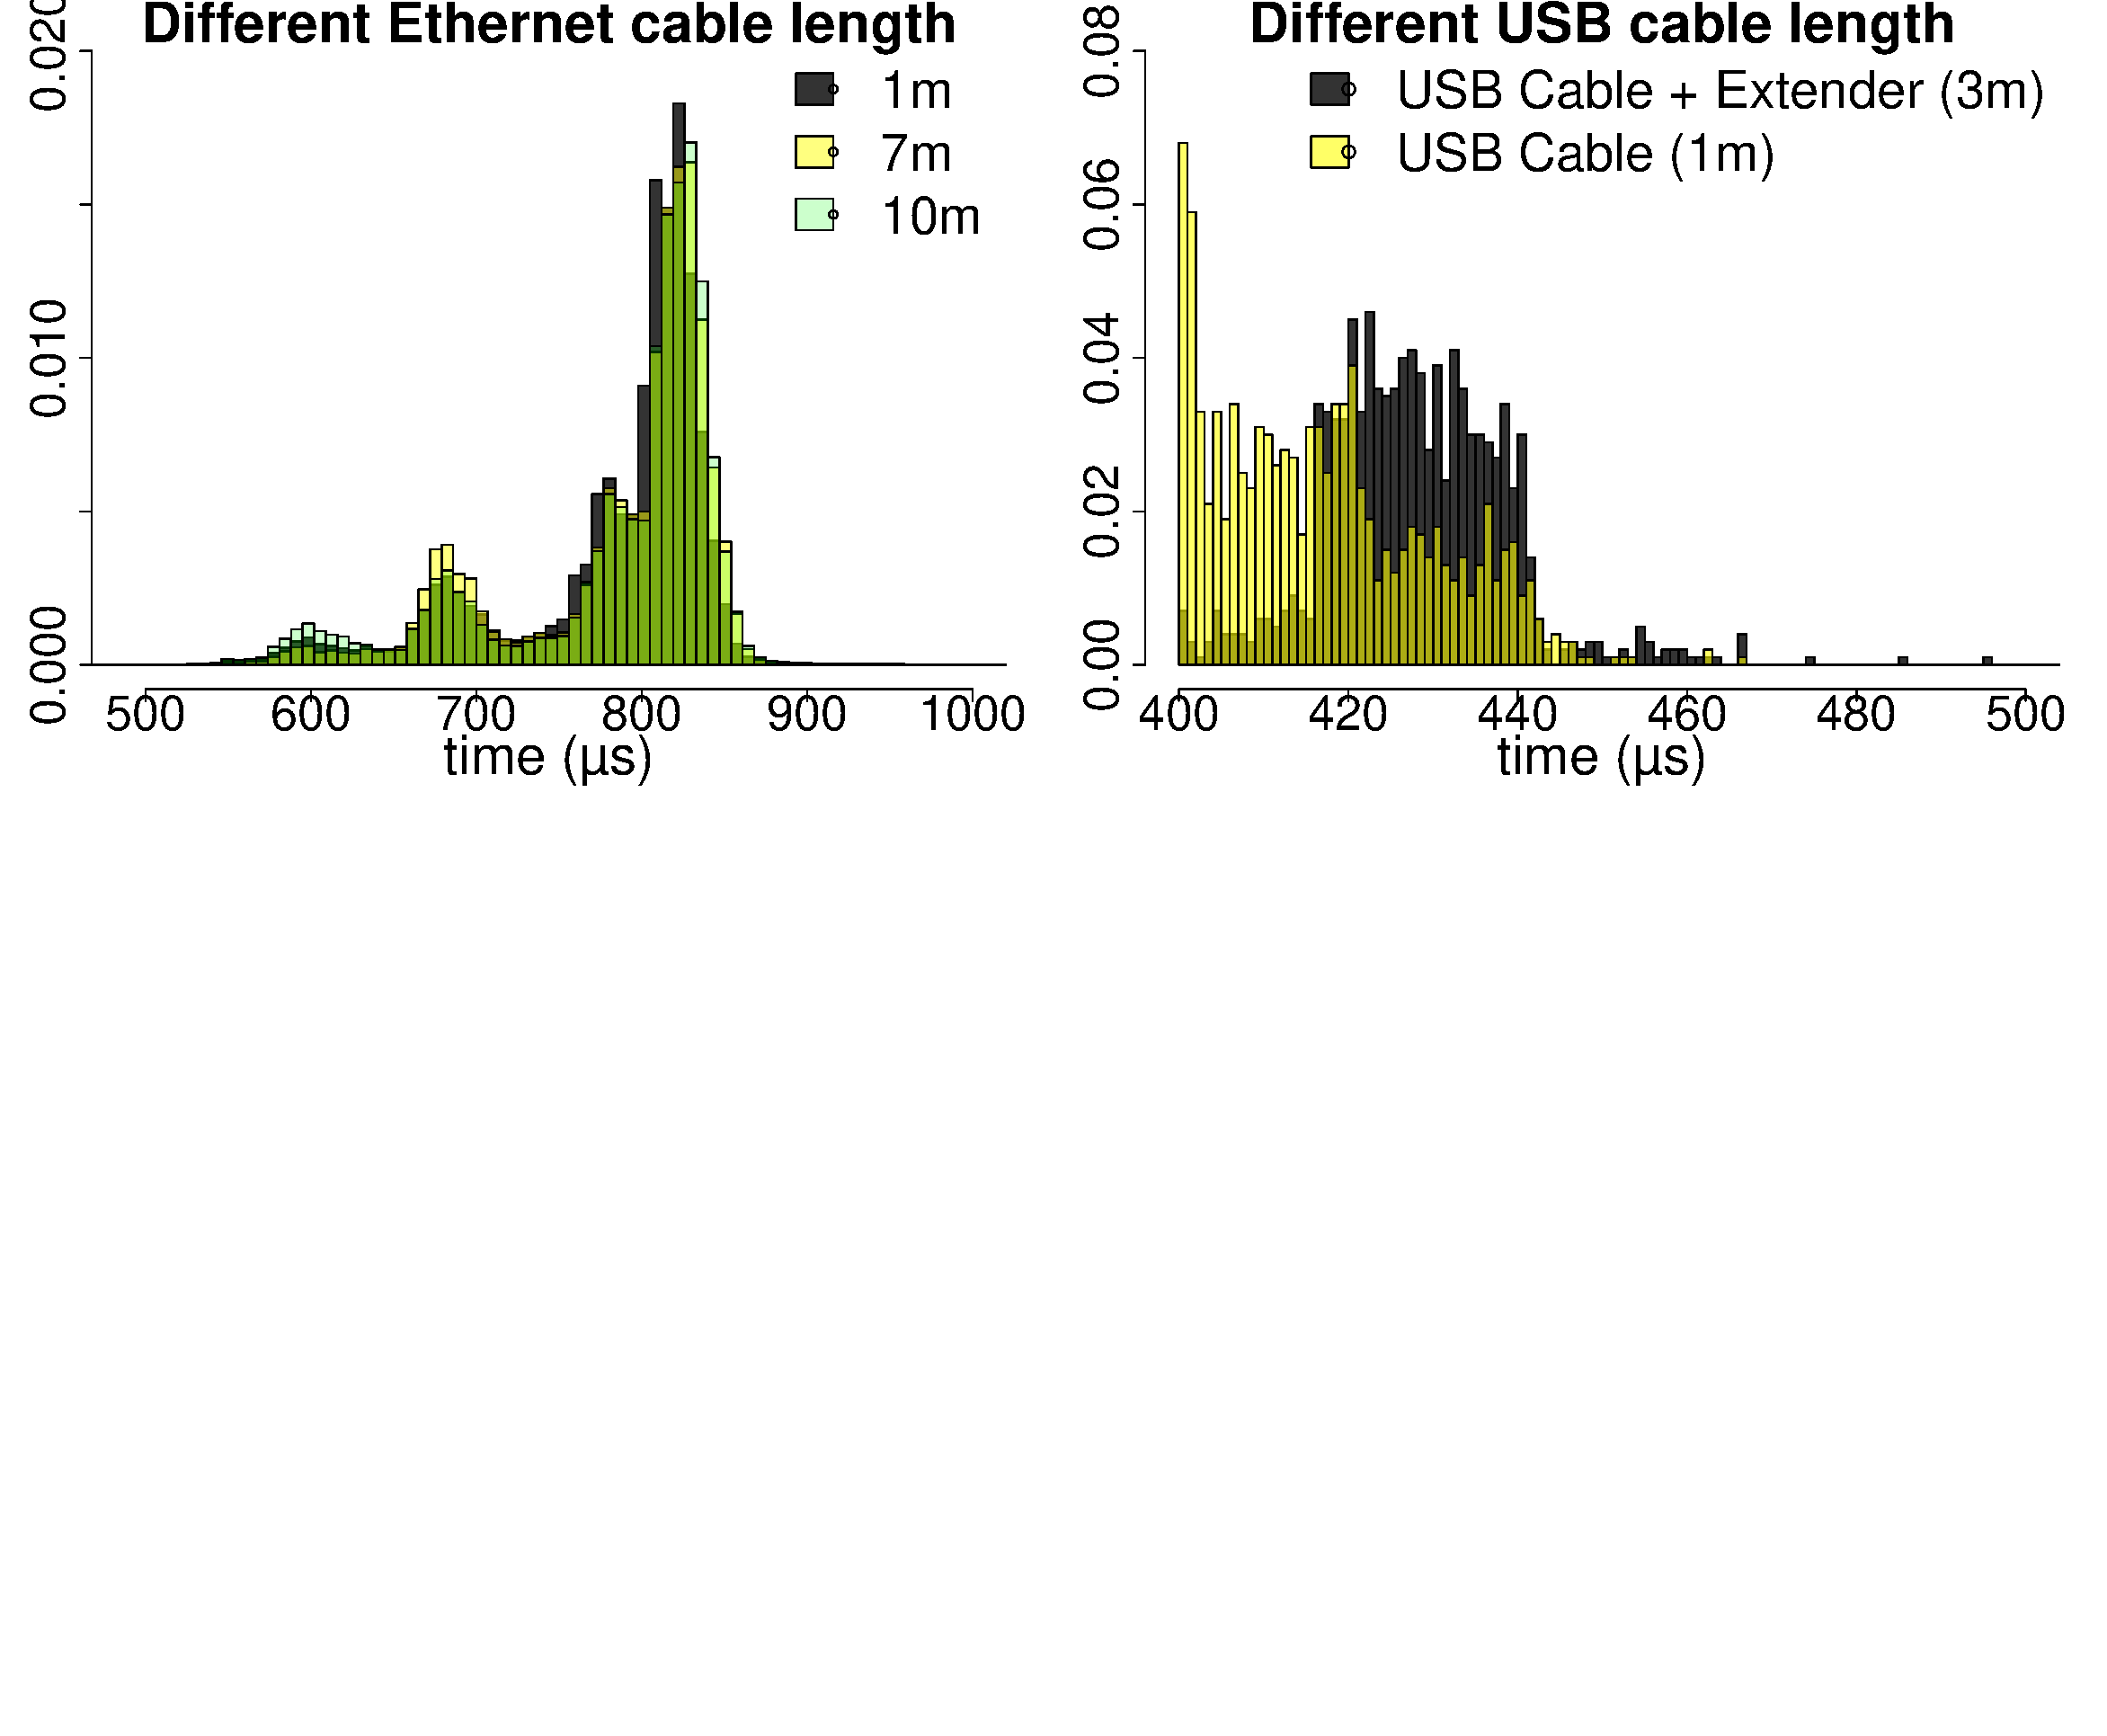
\includegraphics[trim={0 18cm 0 0}, clip, width=\linewidth]{chapters/ProximiTEE/data/graph/CombinedCable_1.pdf}
    \caption[Effect of Different Ethernet/USB cables on the latency]{\textbf{Effect of different Ethernet/USB cables on the latency.} We evaluated latencies two different USB cables: one with an \usb cable (1m) and another with an \usb extender of length 2m attached. Additionally, we evaluated latencies using three different Ethernet cables (1, 7 and 10 m). Latencies are consistent. Note, that the latency is sampled in the experiment conducted with non-\texttt{ping} flood mode.}
    \label{graph:usbCableLength}
\end{figure}


Here we provide results from additional experiments.

We evaluated the consistency of measured latencies across different computing platforms. Figure~\ref{graph:sgxLatency} shows the frequency distribution of latencies across three SGX platforms and three \device devices. We conclude that measurements are consistent result across devices. The two Intel NUCs are few microseconds faster than the Dell Latitude laptop. Additionally, we evaluated the effect of two different \usb cable lengths (3m and 1m) and three different Ethernet cables (lengths of 1m, 7m, and 10m). Figure~\ref{graph:usbCableLength} shows (on the right) that the \usb cable has very small effect on the latency (around 10 $\mu s$ average difference). It also shows (on the left) no significant differences between the different Ethernet cable lengths. 


\begin{figure}[t]
  \centering
    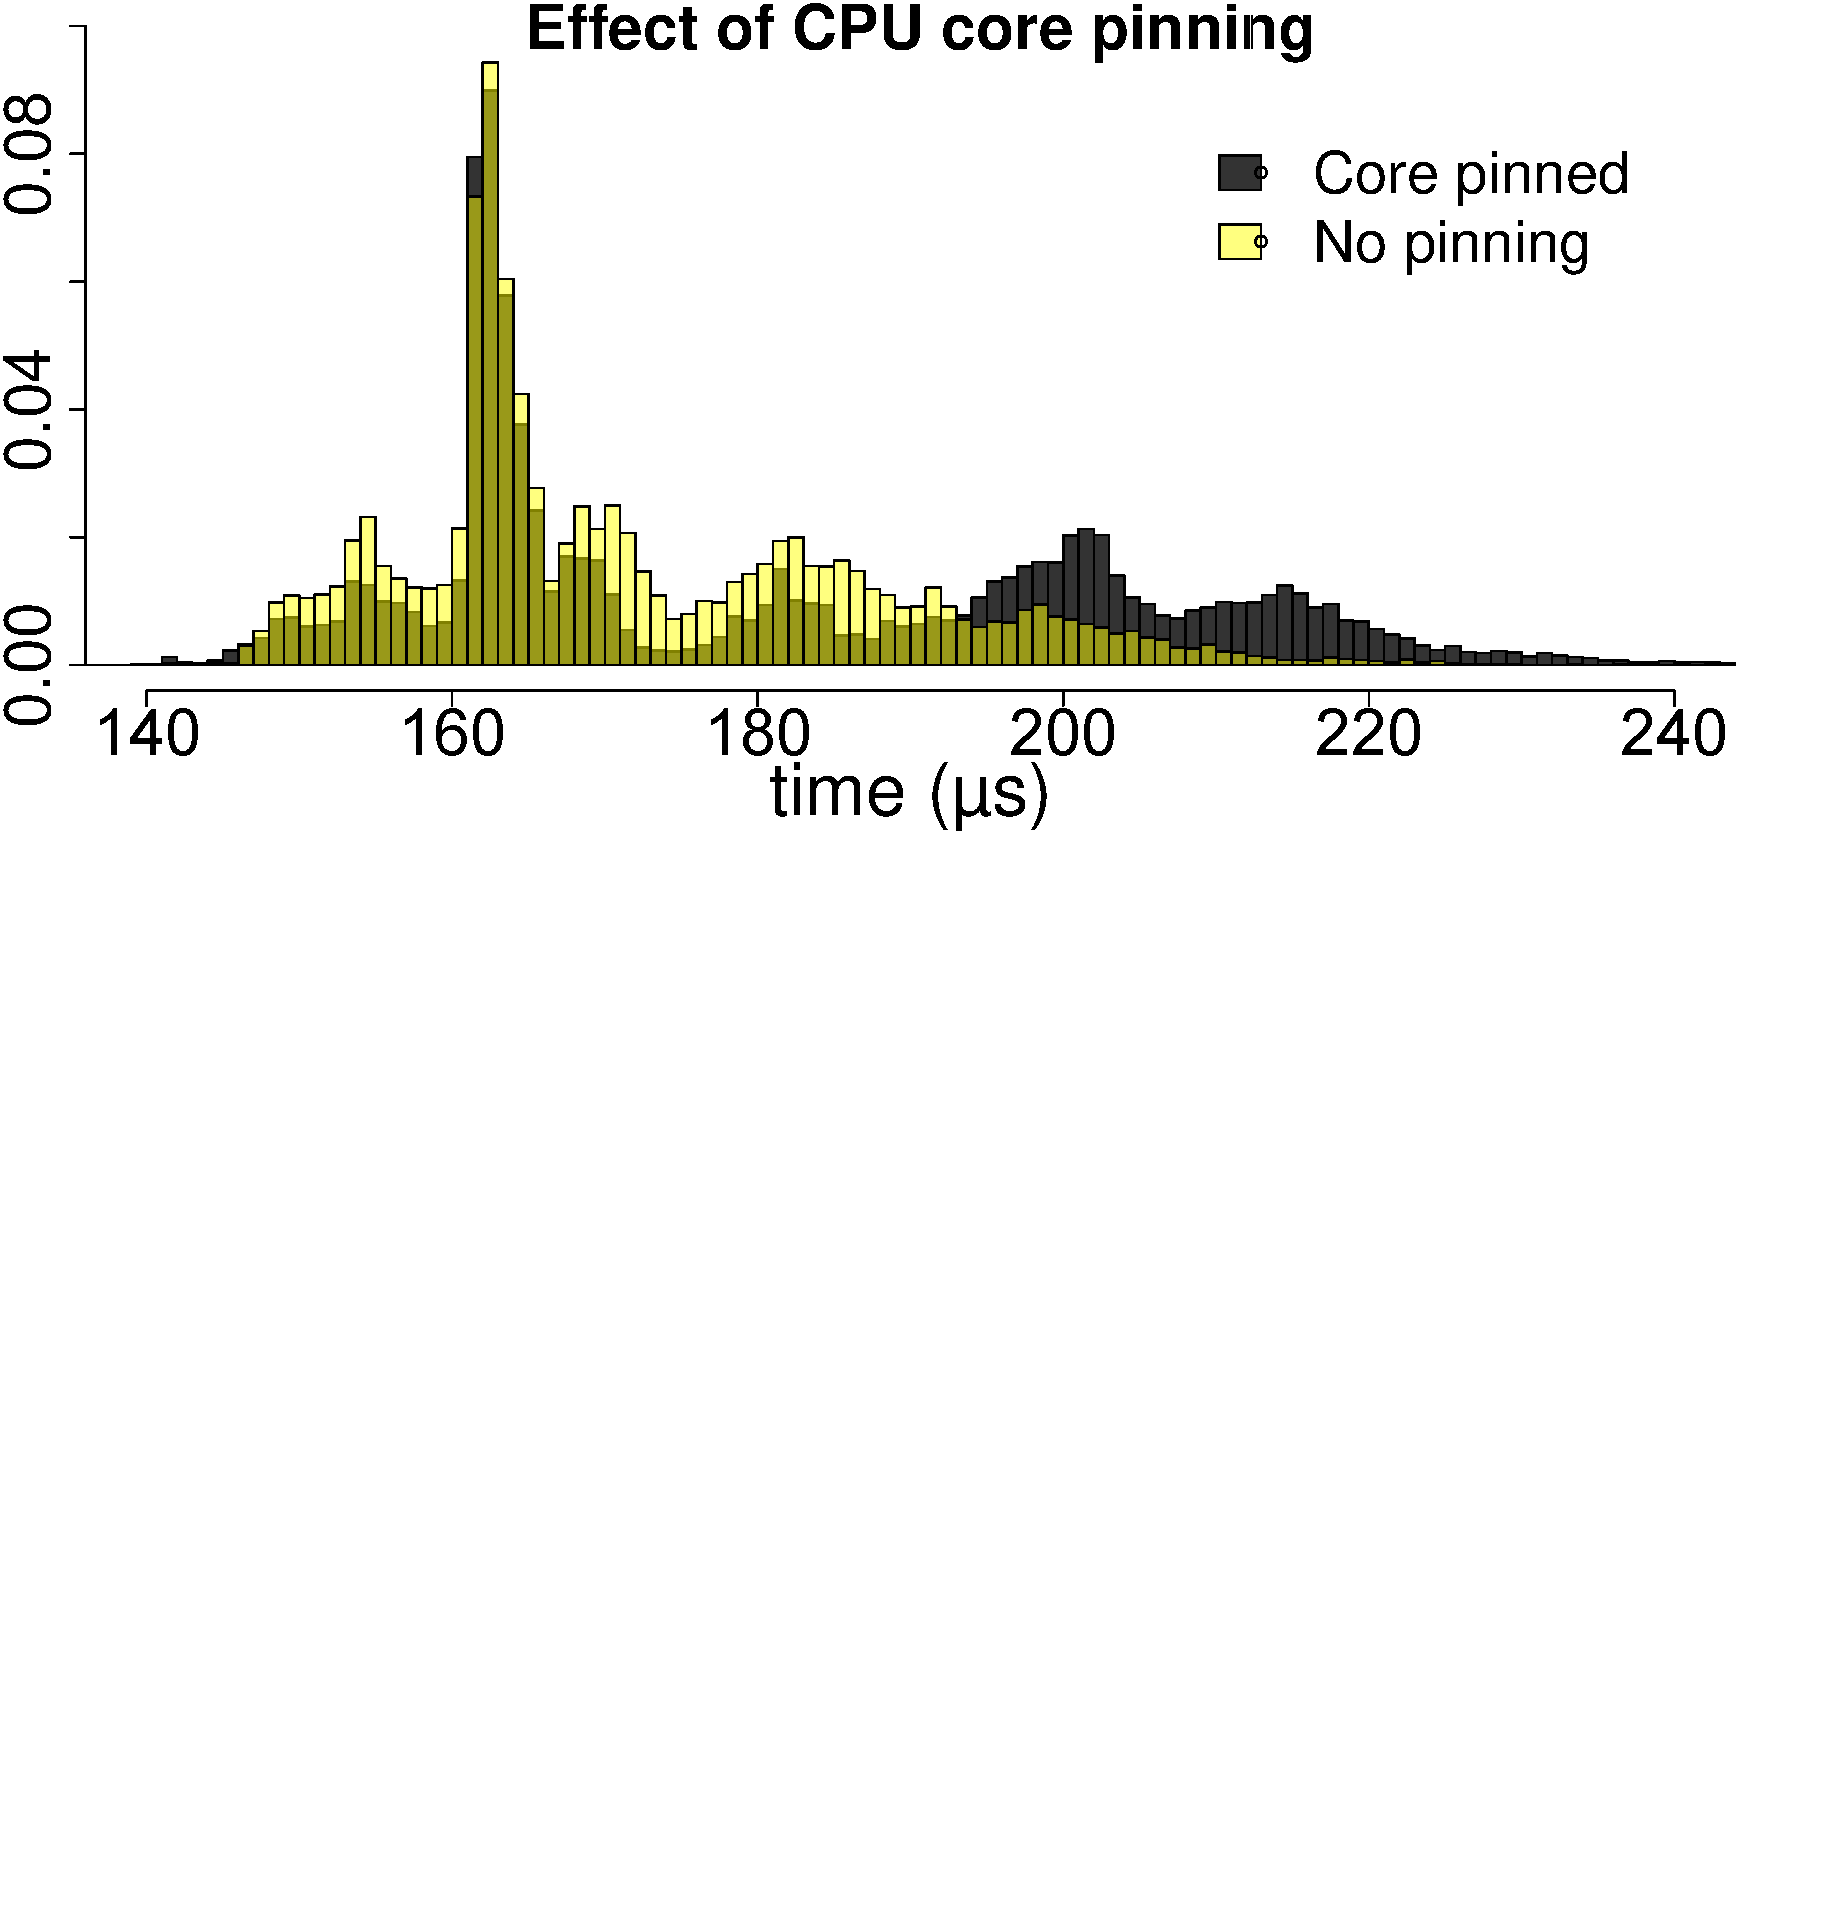
\includegraphics[trim={0 18cm 1.8cm 0}, clip, width=0.75\linewidth]{chapters/ProximiTEE/data/CPU_stress/plot_pin_1.pdf}
    \caption[Effect of CPU core pinning on the enclave application]{\textbf{Effect of CPU core pinning on the enclave application.} Restricting the enclave application to a specific core has a very minor effect on the observed latency.}

    \label{graph:cpuPin}
\end{figure}

\subsubsection{Effects of core pinning.} We executes the \name enclave application pinning to specific CPU cores (using the command \texttt{taskset [COREMASK] [EXECUTABLE]}). Core pinning forces the operating system to use a specific set of CPU core(s) to execute a program. CPU pinning may significantly bring down execution time due to the elimination of core switching and ability to reuse L1 and L2 cache. Figure~\ref{graph:cpuPin} illustrates the effect of CPU core pinning vs. no pinning. We experience negligible effect by core pinning. Hence we conclude that the attacker won't gain any advantage by CPU core pinning.

\begin{figure}[t]
  \centering
    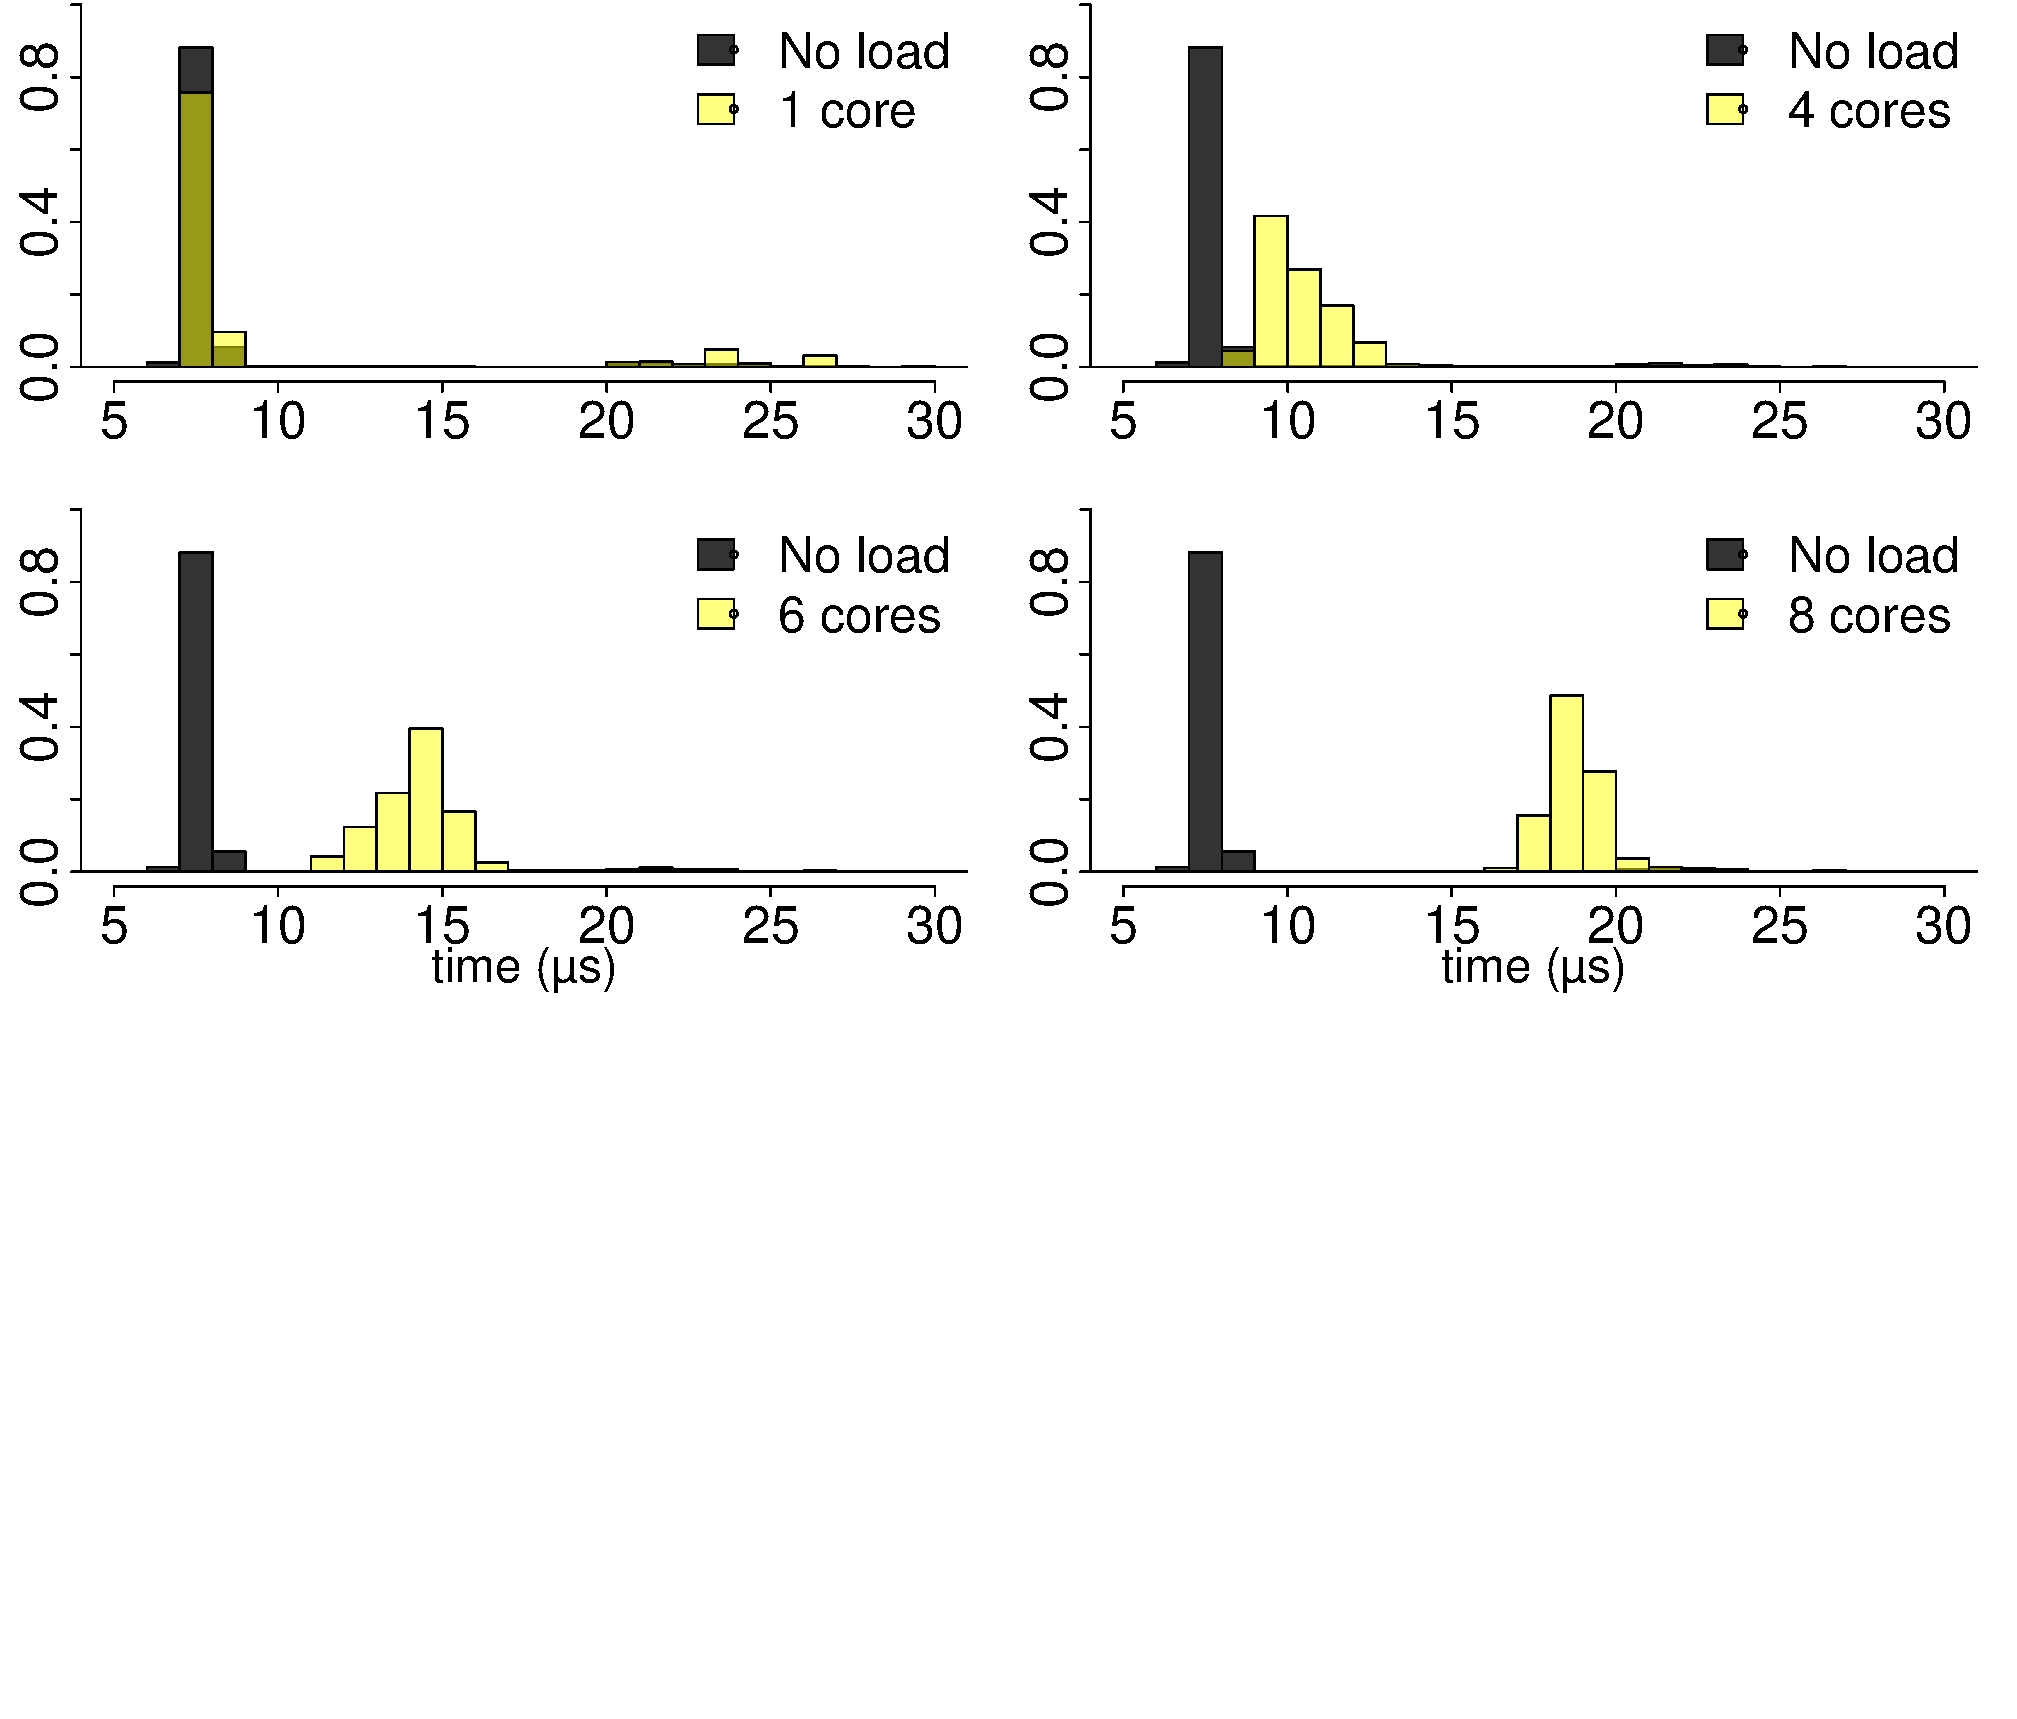
\includegraphics[trim={0 12cm 0 0}, clip, width=0.8\linewidth]{chapters/ProximiTEE/data/CPU_stress/allCore_SGX_1.pdf}
    \caption[Effect on latency experienced by the \device with different number of stressed CPU cores]{\textbf{Effect on latency experienced by the \device with different number of stressed CPU cores.} We evaluated latencies while running CPU intensive benchmark on different number of cores. Note that with higher number of busy cores, the means of the  distributions start to shift towards right but stayed within \connect $= 186\mu s$. We used \texttt{stress-ng} Linux stress-testing application.}
    \label{graph:cpuLoad_SGX}
\end{figure}


\subsubsection{Effects of CPU load.} Figure~~\ref{graph:cpuLoad_SGX} shows the enclave execution times with varying degree of CPU stress testing. We used \texttt{stress-ng} to stress different number of CPU cores. We experienced a minor slowdown with the increasing number of busy CPU cores. But the slowdown is insignificant. For example, as shown in the Figure~\ref{graph:cpuLoad_SGX}, we experienced a shift of $12\mu s$ when all the 8 CPU cores are busy executing the benchmark software. Also, note that the load introduced by the benchmark is a sustained load on all the CPU cores which is much more demanding for the CPUs compared to the CPU loads introduced by real-life applications. In that scenarios, the deviation would be even lesser. We conclude that proximity verification for SGX enclaves is reliable even under high system load. In rare cases of extreme system load, proximity verification might fail, but this is an availability concern, not a security threat.


\subsection{Preventing Relay to Co-Located Platform}
\label{sec:co-located}

The main purpose of our experimental evaluation was to show that our inexpensive \name prototype can effectively prevent relay attacks where the adversary redirects the attestation to another platform that is under his physical control in a \emph{different location}. Next, we discuss whether \name can prevent attestation redirection a \emph{co-located} platform, like another server on the same server rack.

If the two co-located platforms are connected through traditional networking technologies like Ethernet (as in our experiments), our evaluation already shows that such relay attacks can be effectively prevented, using a simple and inexpensive embedded device like our prototype. However, in some modern data centers, computing platforms are connected with faster inter-connect technologies like InfiniBand connections that can enable latencies as lows as $7 \mu$s~\cite{liu2003performance}. 

The ability to distinguish relay attacks depends on three key factors. The first is the latency of the channel through which the relay is performed (e.g., $7 \mu$s for InfiniBand). The second is the time required to compute responses to challenges on the target platform (e.g., $6-10 \mu$s in the SGX platforms that we tested). And the third is how much variance the round-trip times between the embedded device and the target platform have (e.g., $10-20 \mu$s in our USB 3.0 prototype). The local communication variance and the response computation time should be less than the relay latency, to enable robust proximity verification. 

We conclude that our simple prototype cannot prevent all possible relays to co-located platforms when very fast inter-connect technologies like InfiniBand are used. To address such relay attacks, one needs a faster and more accurate embedded device that exhibits less variance. For example, PCIe connected FPGAs can have latencies as lows $1 \mu $s~\cite{algoLogic}. Besides better embedded device, one can also increase the number of distance-bounding protocol rounds and reduce the success probability for legitimate attestation $P_{legit}$.



\section{Addressing Emulation Attacks}
\label{sec:variantII}

We consider attestation key extraction from SGX processors difficult and rare, in contrast to the previously considered relay attacks that require only OS control or other malicious software on the target platform. However, the recently demonstrated Foreshadow attack~\cite{foreshadow-usenix18} that exploited the Meltdown vulnerability~\cite{Lipp2018meltdown} showed how to extract attestation keys from SGX processors. Although Intel has the possibility to issue microcode patches that address processor vulnerabilities like Meltdown and the processor's microcode version is reflected in the SGX attestation signature, new vulnerabilities like the ZombieLoad attack~\cite{ZombieLoad} may be discovered. Before microcode patches are deployed, in rare occasions, leaked but not revoked attestation keys may be available to the attacker.


\subsection{Addressing the Emulation Attack} 

\myparagraph{attacker model} 
We consider an \emph{emulation attacker} has all the capabilities of the relay attacker (cf.\ Section~\ref{sec:problemStatement}) and additionally has obtained at least one valid (not yet revoked by Intel) attestation key from any SGX platforms but the target platform. The attacker might obtain an attestation key by attacking one of his processors or by purchasing an extracted key from another party. 

\myparagraph{The emulation attack} 
In the attack, the attacker uses a leaked attestation key to emulate an SGX-processor on the target platform. Since the IAS (or any other attestation service) successfully attests to the emulated enclave, it is impossible for the remote verifier to distinguish between the emulated enclave and the real one. 


\myparagraph{Emulation attack implications} 
The emulation attack allows the attacker to fully control the attested execution environment and thus break the two fundamental security guarantees of SGX, enclave's data confidentiality and code integrity, and to access any secrets provisioned to the emulated enclave. Since the OS is also under the control of the attacker, any attempted communication with the real enclave will always be redirected to the emulated enclave.



\begin{figure}[t]
 \centering
%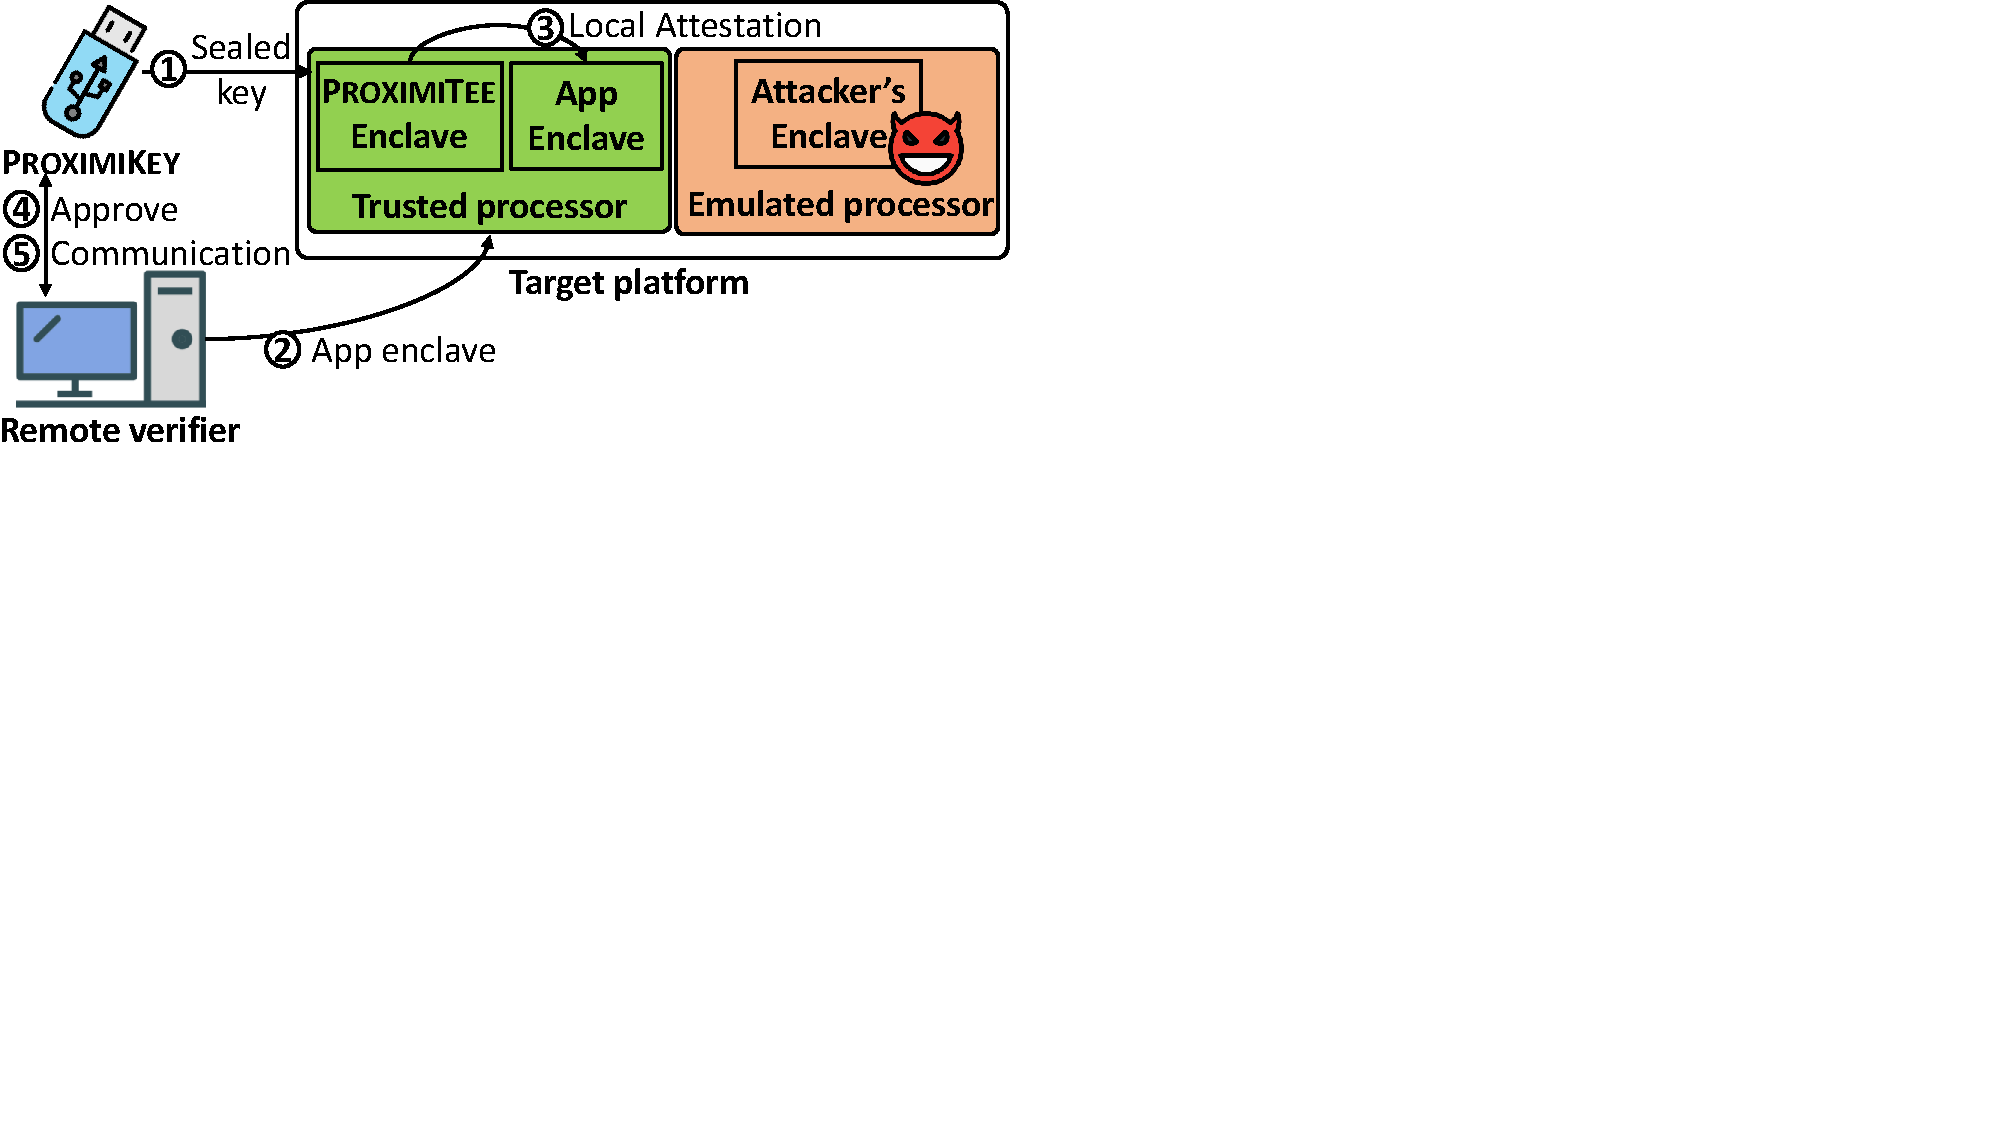
\includegraphics[trim={0 11.6cm 16.5cm 0},clip,width=0.72\linewidth]{chapters/ProximiTEE/figures/boot-attest.pdf}
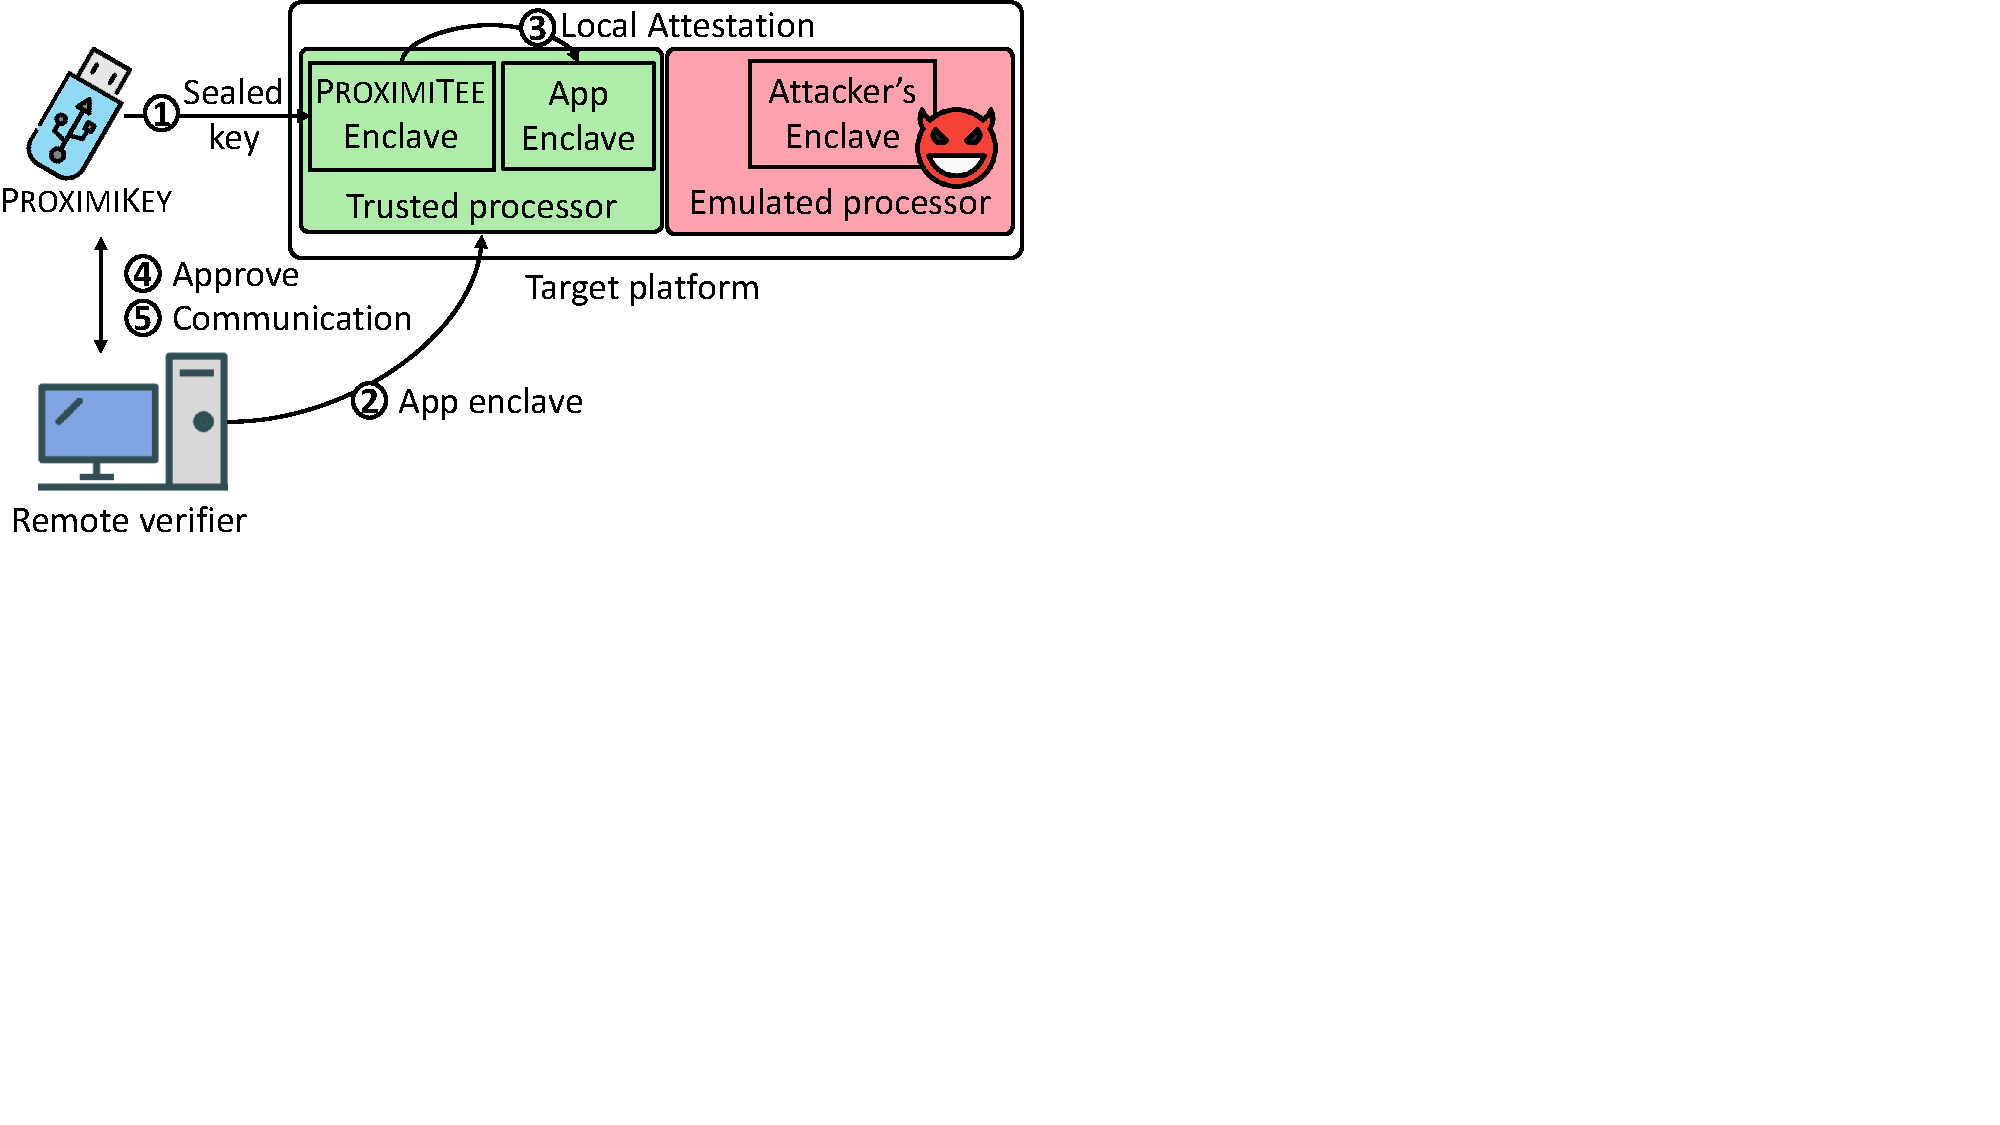
\includegraphics[trim={0 9cm 16.5cm 0},clip,width=0.72\linewidth]{chapters/ProximiTEE/images_new/boot_attest.pdf}
 \caption[\name boot-time attestation]{\textbf{\name boot-time attestation.} After the boot-time initialization (refer to Figure~\ref{fig:boot-init}) the \nameclave executes a local attestation with the verifier uploaded \app. 
 }
 \label{fig:boot-attest}
\end{figure}


\begin{figure}[t]
 \centering
    %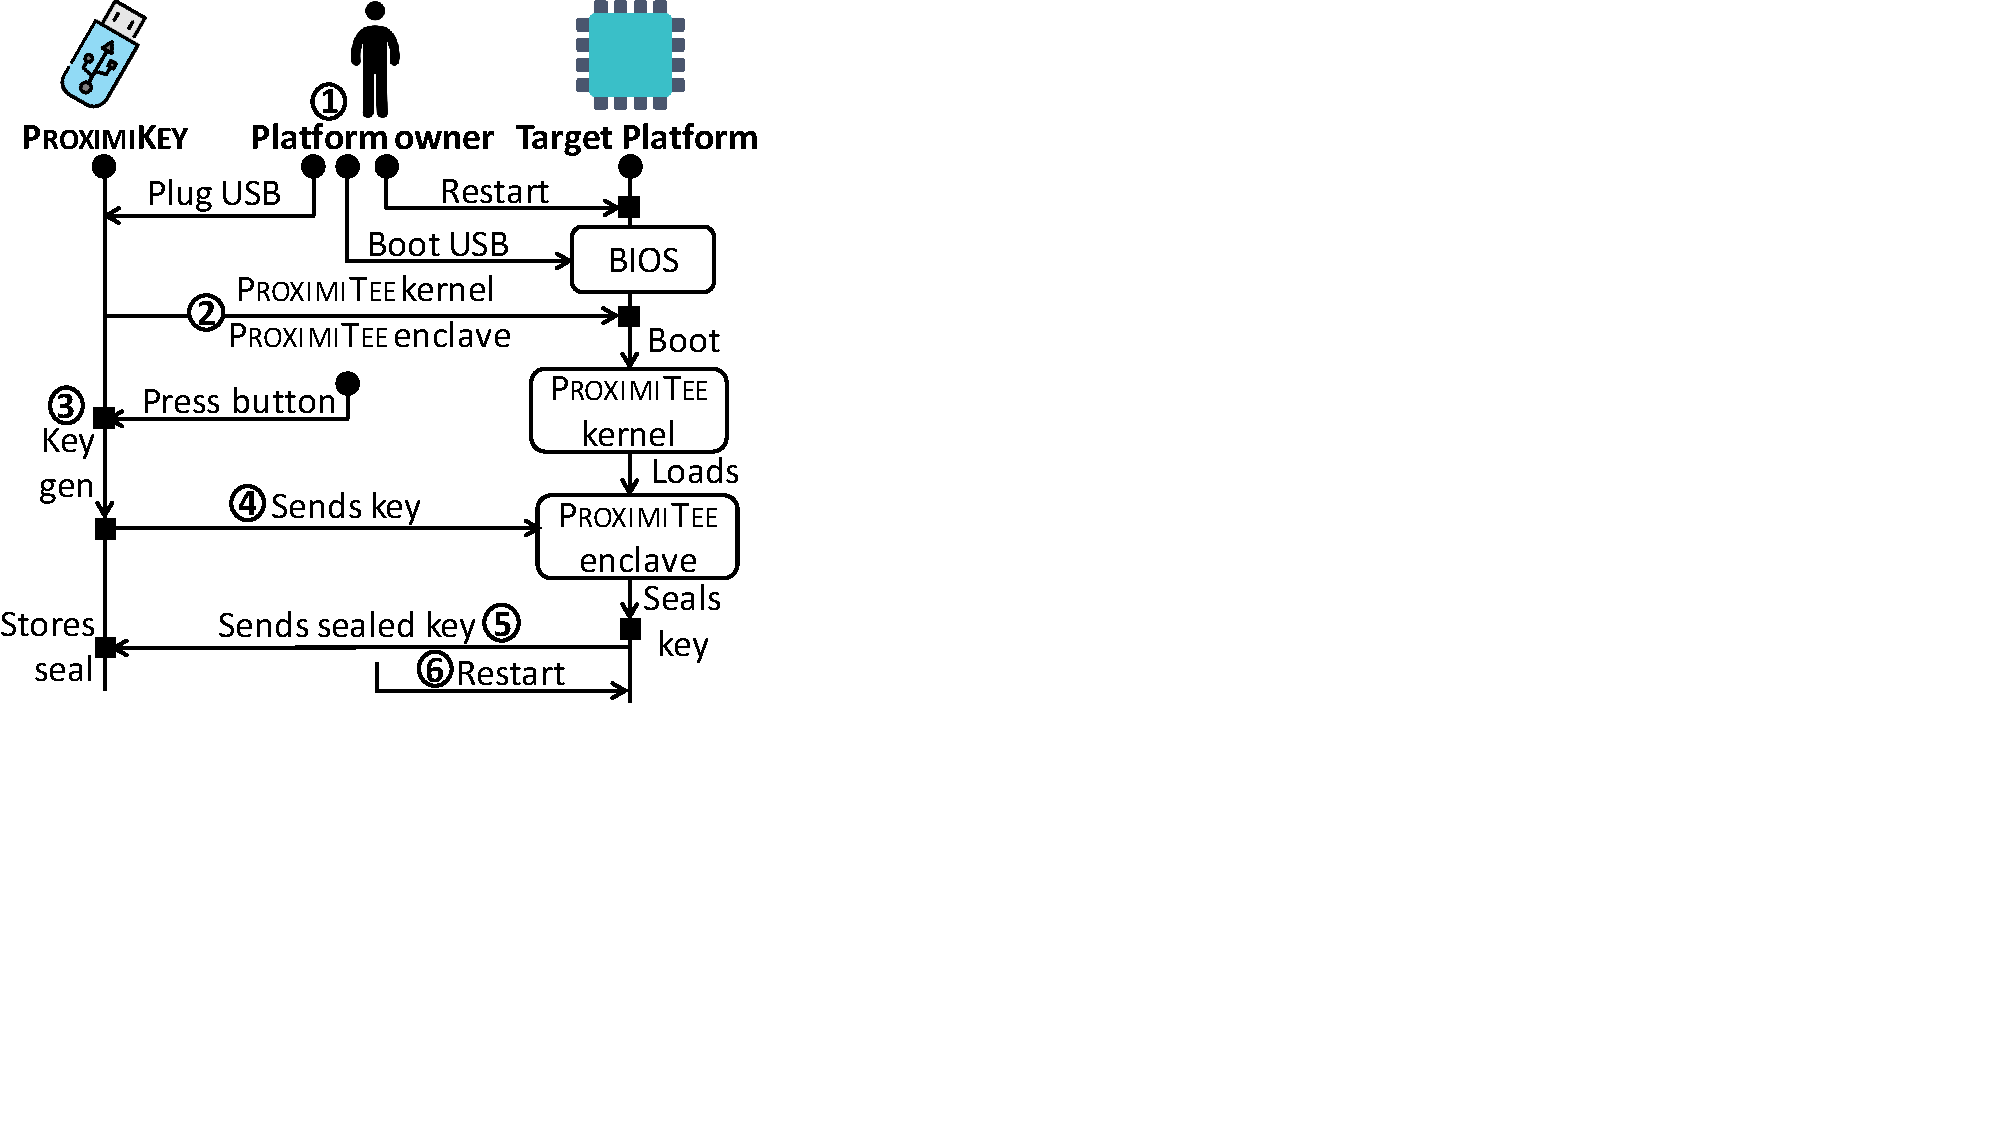
\includegraphics[trim={0 7cm 19cm 0},clip,width=0.7\linewidth]{chapters/ProximiTEE/figures/boot_init.pdf}
    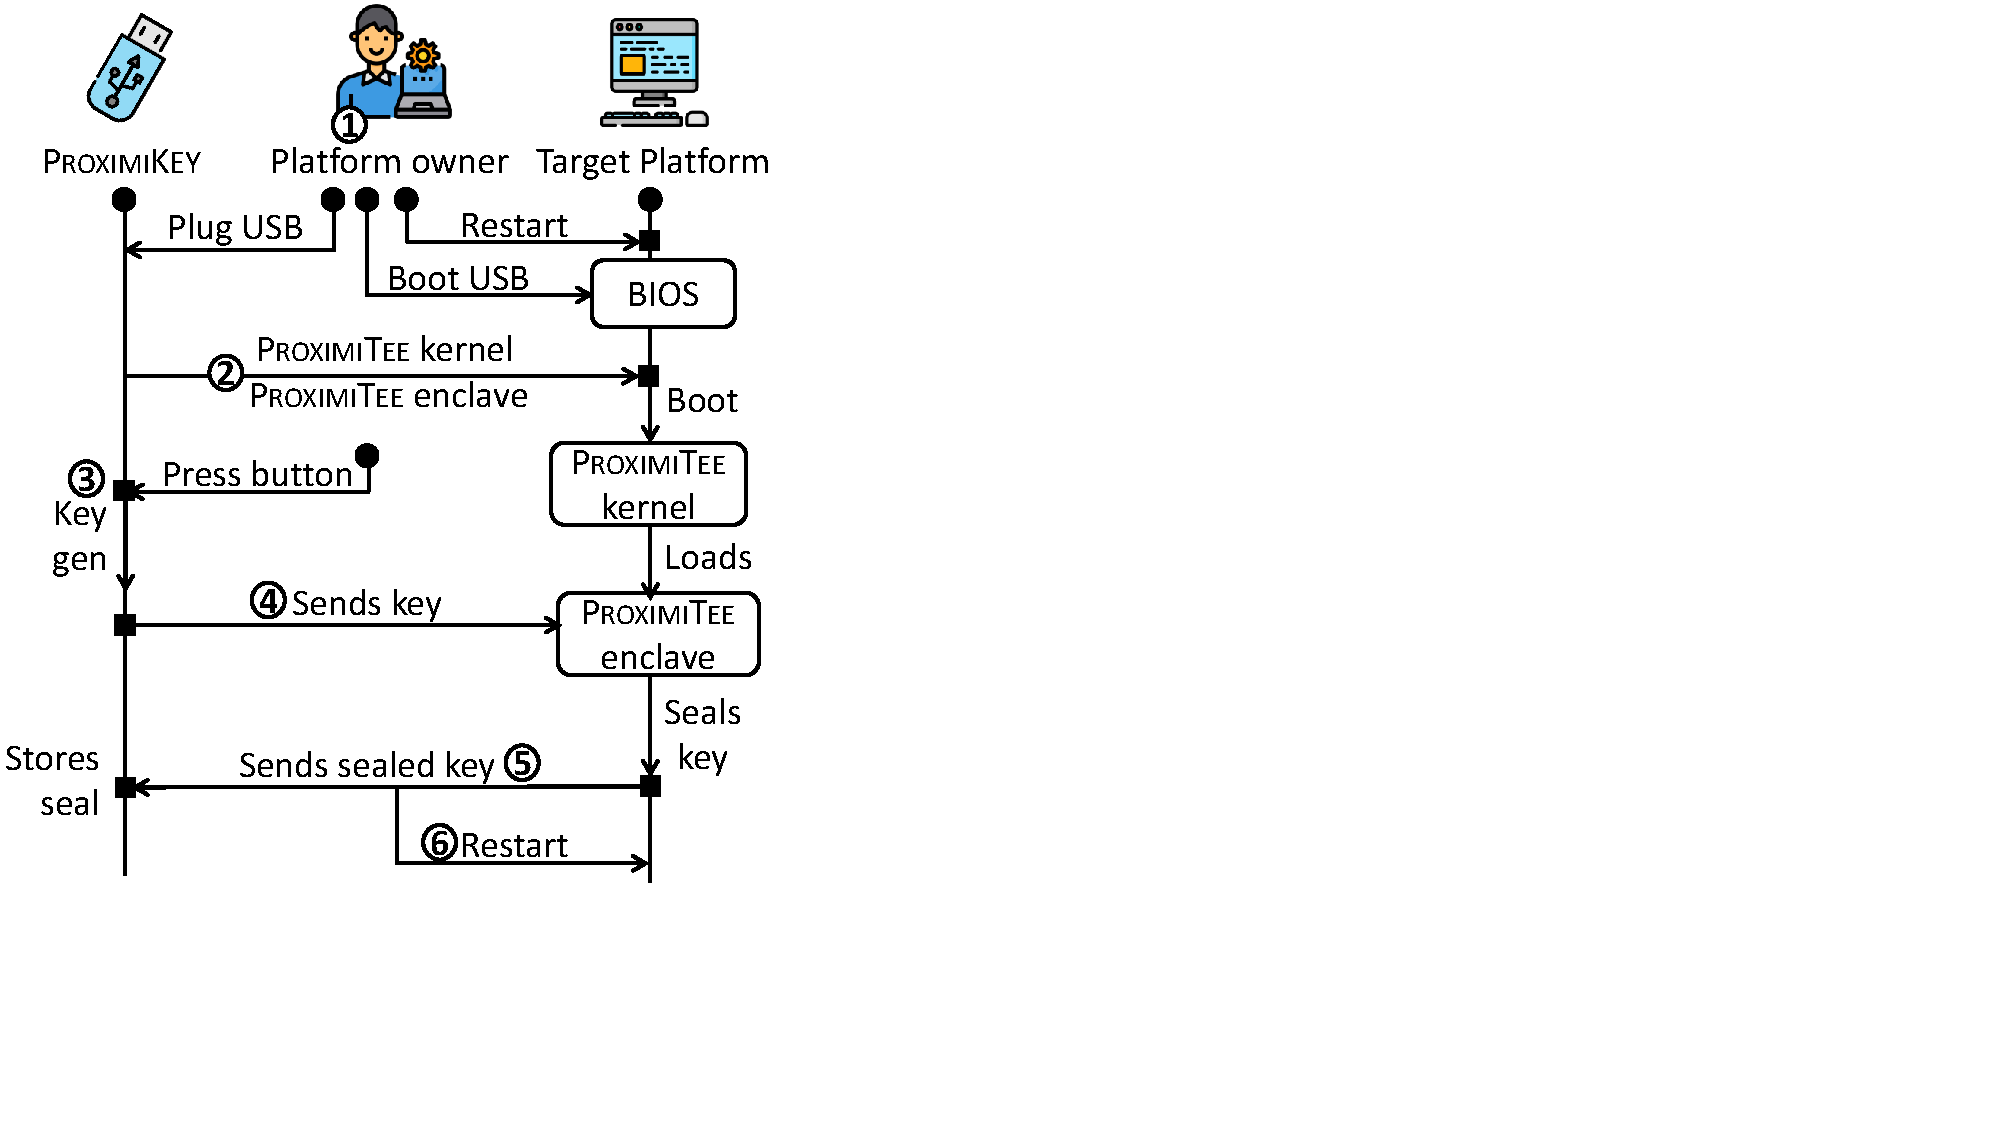
\includegraphics[trim={0 2cm 19cm 0},clip,width=0.7\linewidth]{chapters/ProximiTEE/images_new/boot_init.pdf}
 \caption[\name noot-time initialization]{\textbf{\name boot-time initialization.} The \device uses a minimal kernel Linux image to boot and load \nameclave on the target platform and seal a platform specific secret to the \device{}'s memory.}
 \label{fig:boot-init}
\end{figure}



\subsection{Boot-Time Initialization Solution}

Proximity verification alone cannot protect against the emulation attacker, as the locally emulated enclave would pass the proximity test. 
%
Therefore, we describe a second hardened attestation mechanism that leverages secure boot-time initialization and is designed to prevent emulation attacks. This solution can be seen as a \emph{novel variant} of the well-known TOFU principle, and the main benefit of our solution over previous variants is that it simplifies deployment and increases security. Additionally, when such attestation is used in combination with our previously described periodic proximity verification, our solution enables secure offline revocation.


\myparagraph{Security assumptions}
Our security assumptions regarding the target platform are as described in Section~\ref{sec:problemStatement}. The only difference is that in this case, we assume that the UEFI (or BIOS) on the target platform is trusted.


\myparagraph{Solution overview}
Figure~\ref{fig:boot-attest} illustrates an overview of this solution. During initialization, that is depicted in Figure~\ref{fig:boot-init}, the target platform is booted from the attached device that loads a minimal and single-purpose \name kernel on the target device. In particular, this kernel includes no network functionality. The kernel starts the \name enclave, which shares a secret with the device. This shared secret later bootstraps the secure communication between \device and the \name enclave. \emph{The security of the bootstrapping relies on the fact that the minimal kernel will not perform enclave emulation at boot time.} The \name enclave will later be used as a proxy to attest whether other (application-specific) enclaves in the system are real or emulated and on the same platform.


\myparagraph{Boot-time initialization} The boot-time initialization process is performed only once.
This process is depicted in Figure~\ref{fig:boot-init} and it proceeds as follows:


\begin{enumerate}
  \item[\one] The platform owner plugs \device to the target platform, restarts it to BIOS and selects the option to boot from \device.
  \item[\two] \device loads the \name kernel and boots from it. The \name kernel starts the \nameclave.
  \item[\three] The user presses a button on \device to confirm that this is a boot-initialization process. This step is necessary to prevent an attack where the compromised OS emulates a system boot.
  \item[\four] \device sends a randomly generated key $\mathcal{K}$ to the \nameclave.
  \item[\five] The enclave returns the sealed key $\mathcal{S}$ corresponding to the key $\mathcal{K}$ ($\mathcal{S}\leftarrow\texttt{Seal}(\mathcal{K})$) to \device that stores the key and the seal pair $(\mathcal{K}, \mathcal{S})$ on its flash storage.
  \item[\six] \device blocks further initializations, sends a restart signal and boots the platform with the normal OS.
\end{enumerate}


\myparagraph{Attestation process} After initialization the target platform runs a regular OS. The attestation process is depicted in Figure~\ref{fig:boot-attest} and proceeds as follows:

\begin{enumerate}


  \item[\one] \device sends the seal $\mathcal{S}$ to the \nameclave that unseals it and retrieves the key $\mathcal{K}$. \device and the \nameclave establish a secure channel (\tls) using $\mathcal{K}$.

  \item[\two] The remote verifier uploads a new \app on the target platform.

  \item[\three] The \nameclave performs local attestation (refer to~Section~\ref{ch:background:SGX:local}) on the \app that binds its public key to the attestation. %The local attestation ensures that i) the \app is on the same physical platform, and ii) the code integrity of the \app.

  \item[\four] The \nameclave sends the measurement and the public key of the \app to \device. \device establishes a secure channel to the \app and sends the measurement of the enclave to the remote verifier. The remote verifier then approves the communication to the \app.

  \item[\five] The remote verifier checks that the measurement of the \app is as expected. If this is the case, it can communicate with the enclave through \device.


\end{enumerate}


\myparagraph{Following communication} 
Similar to our previous solution, after the initial attestation, all the communication between a remote verifier and the enclave is mediated by the \device that periodically checks the proximity of the attested enclave and terminates the communication channel in case the embedded device is detached.


\subsection{Security Analysis and Implementation}
 
In this attestation mechanism, the task of establishing a secure communication channel to the correct enclave can be broken into three subtasks. The first subtask is to establish a secure channel to the correct \device device. In our solution, this is achieved using standard device certification. Recall that the attacker cannot compromise the specific \device used. 

The second subtask is to establish a secure communication channel from \device to the \nameclave. \device shares a key with an enclave that is started by the trusted \name kernel, hence at a time in which the attacker could not emulate any enclave. \device knows when secure initialization takes place as the platform owner indicates this by pressing a button -- an operation that the attacker cannot perform. The \nameclave seals the key during initialization. Different SGX CPUs cannot unseal each other's data, and therefore even if the attacker has extracted sealing keys from other SGX processors, she cannot unseal the key and masquerade as the legitimate \nameclave. 

The third subtask is to establish a secure communication channel from the \nameclave to the \app. The security of this step relies on SGX's built-in local attestation. An attacker in possession of leaked sealing attestation keys from other SGX processors cannot produce a local attestation report that the \name enclave would accept, and therefore the attacker cannot trick the remote verifier into establishing a secure communication channel to a wrong enclave.


\myparagraph{Comparison to TOFU} Our second attestation mechanism is a novel variant of the well-known ``trust on first use'' principle. In this section, we briefly explain the main benefits of our solution over common TOFU variants. 

\begin{enumerate}
\item \emph{Smaller TCB size and attack surface.} 
In the TOFU solution, the standard and general-purpose OS needs to be trusted on first use, and the CA needs to remain online for enrollment of new SGX platforms. In our solution, a significantly smaller and single-purpose kernel needs to be trusted on first use. Additionally, we require trust in the BIOS (or UEFI). In our solution, the CA can remain offline when a new platform is enrolled.


\item \emph{Reboot instead of reinstall.} Our solution requires that the target platform is rebooted once from \device. In most TOFU solutions, the target platform requires a clean state which is difficult to achieve without reinstall that makes deployment difficult.


\item \emph{Secure offline revocation.} When boot-time initialization is combined with the previously explained periodic proximity verification, our solution provides an additional property of secure offline revocation that requires no interaction with the CA. Such property is missing from previous TOFU solutions.

\end{enumerate}

\myparagraph{Implementation} We implemented a complete prototype of our second attestation mechanism. On top of our previous \name implementation (refer to Section~\ref{sec:implementation}), the boot-time initialization solution requires the \name kernel. We have modified an image of Tiny Core Linux~\cite{tinyCore} and used it as the boot image for our boot-time initialization. The image size of our modified Linux distribution is 14 MB (in contrast to 2 GB standard 64 bit Linux images build on the standard kernel). Our image supports bare minimum functionality and includes \texttt{libusb}, \texttt{gcc}, Intel SGX SDK, Intel SGX platform software (PSW), and Intel SGX Linux driver. The \name enclave is a minimal enclave that uses a simple serial library to communicate with the \device and local attestation mechanism to attest any application-specific enclave.

%!TEX root =  ../paper.tex

\section{Discussion and Related Work}
\label{sec:discussion}

%\parasaver
\myparagraph{Extension to other TEEs} Our approach could be applied to other TEEs as well. The critical requirements for the TEE is that it must support programmable operations that can be executed sufficiently fast. One TEE that meets these requirements is ARM TrustZone. %We consider adapting our solution for TrustZone an interesting direction for future work.


\vspace{-2pt}
\myparagraph{DRTM proximity verification}
Presence attestation~\cite{presenceAttestation} enables proximity verification DRTM-based TEEs~\cite{mccune2008flicker}. The TEE shows an image that is captured by a trusted camera and communicated to a remote verifier. The same approach cannot be used with SGX since it lacks trusted path for secure image output. Catching the cuckoo~\cite{CatchingCuckoo} uses timing side channel to verify proximity with a TPM emulator. The TPM latency is in the order of seconds, making it invisible for any practical distance bounding. 

%\section{Related Work}
\label{sec:relatedWork}

In this section, we discuss some of the most relevant works to \name. We also discuss the main differences with \name to these works.


\subsection{TEE-based solutions}
There exist several solutions for integrating external devices to widely deployed TEEs: Intel SGX, and ARM TrustZone. 

\myparagraph{SGXIO} SGXIO is a proposal by Weiser et al.~\cite{weiser2017sgxio} that builds on top of Intel SGX, intending to allow SGX to interact with input-output devices. They achieve that by introducing a trusted hypervisor that allows enclaves to access virtualized peripherals. Similar to our approach, SGXIO also considers a remote adversary. However, SGXIO is rather static in nature, i.e., all the peripherals have to be set up at boot time. After the system setup phase, no changes are allowed (connect new peripherals, etc.). It is not clear how enclaves are created and get access to a peripheral while preserving the confidentiality of previous enclaves that used said peripheral. Essentially, SGXIO allows for a static extension of the hardware TCB.

\myparagraph{Graviton and systems based on it} Graviton~\cite{volos2018graviton} is a TEE that runs on an accelerator such as a graphics card. It can provide isolation between the data of multiple stakeholders that run tasks on the GPU concurrently. It also provides remote attestation of an enclave on the accelerator. Graviton was evaluated on a modern graphics card and shows that the predominant overhead stems from encryption of the communication to the processor. However, they also demonstrate that the overhead of around 20\% is tolerable. Graviton would fit very well within a \name{} as it is an excellent example of an enclave on a peripheral. It provides isolation for secret data and attestation reports. In addition, it shows that even some of the most powerful accelerators can be extended with a local TEE. Visor~\cite{visor} is a system built upon Graviton~\cite{volos2018graviton} that proposes a hybrid TEE that spans over both CPU and GPU. Visor is aimed towards privacy-preserving video analytics where the computation pipeline is shared between the CPU (non-CNN workloads) and the GPU (CNN workloads) to increase efficiency. Visor addresses micro-architectural-based side-channel attacks where a local physical attacker can use the data-dependent memory access patterns (e.g., branch-prediction, cache-timing, or controlled page fault attacks) to reveal elements on the video analysis (e.g., leaks pixel patterns). The communication between the CPU and GPU enclaves is encrypted. Additionally, Visor ensures that the traffic pattern between the CPU and GPU enclaves is independent of the video content.

\myparagraph{HETEE} HETEE~\cite{zhu2020hetee} is another proposal to extend TEEs to accelerators (specifically GPUs) without requiring changes to existing CPUs/GPUs. HETEE focuses on data center applications and proposes an extra hardware box per rack that is protected from physical attacks. This box also contains all accelerators, which it then connects to compute servers in the same rack. Each enclave then runs on a dedicated compute server and a connected accelerator. In essence, the HETEE box provides secure routing of accelerators to dedicated compute servers. In contrast to HETEE, we aim to be able to execute multiple composite enclaves on the same compute server. 


\myparagraph{ARM TrustZone and systems based on it} TrustZone is a system TEE provided by ARM for their system-on-chips (SoC)~\cite{winter2008trusted}. TrustZone applications run on top of a secure OS that is trusted and isolated from the standard operating system (also known as the rich OS). Isolation between the two worlds is achieved by an extra bit on the bus. 
%and some additional configurable components such as the TrustZone Address Space Controller (AZASC). The AZASC is a dedicated hardware component on the SoC that may permit and refuse some access to memory. 
However, there is no isolation between different TrustZone applications. Due to this limitation, mobile phone manufacturers usually only allow TrustZone applications that are signed by them. % --  a restricted version of the local attestation. 
TrustZone only provides the lower level isolation property between the rich OS and the secure OS. Everything else, i.e., isolation between TrustZone applications, remote attestation, etc., has to be added to the secure OS~\cite{ning2014samsungknox}. There have been many proposals that try to improve on the capabilities of TrustZone~\cite{brasser2019sanctuary,hua2017vtz}. Sanctuary~\cite{brasser2019sanctuary} enables user-space TrustZone enclaves. Sanctuary achieves isolation by running enclaves in their own address space in the normal world. However, Sanctuary is very similar to Intel SGX, and thus, it does not extend to peripherals.
%Similar to these proposals, TrustZone could also be extended in the direction of \name{} to support \nameenclave{}s. 
There exist proposals that enable additional security properties such as a trusted path by enabling direct pairing of peripherals (e.g., the touchscreen) to the TrustZone application. Such proposals include TruZ-Droid~\cite{TruZ-Droid}, TrustUI~\cite{trustUI}, SeCloak~\cite{SeCloak}, VButton~\cite{VButton}. All of these solutions do not provide any form of peripheral attestation similar to \name{}. They also do not consider other peripherals or how to dynamically allow an enclave to access a peripheral previously used by another enclave. Moreover, as mentioned earlier, the absence of isolation between the TrustZone applications makes the proposal mentioned above weak in inter enclave isolation guarantee.


\subsection{Other isolation methods} 

Minimal hypervisors or operating systems~\cite{herder2006minix,klein2009sel4} can also achieve isolation, and some are even formally verified~\cite{klein2009sel4}. Usually, such hypervisors do not include attestation, but the cost of adding that should be very low. A \name{} could also be based on a microkernel such as seL4. One would have to add an interface for the malicious OS running in a virtual machine to interact with enclaves that run directly on top of seL4, similar to other pure hypervisor-based isolation systems~\cite{virtualGhost,Overshadow,InkTag,TrustVisor,SplittingInterfaces,terra}. It might even be possible to formally prove such modifications to provide an even stronger assurance of isolation. Similar to other pure hypervisor-based isolation system include Virtual Ghost~\cite{virtualGhost}, Overshadow~\cite{Overshadow}, InkTag~\cite{InkTag}, TrustVisor~\cite{TrustVisor}, Splitting Interface~\cite{SplittingInterfaces}, Terra~\cite{terra} etc.  The hypervisor is also in charge of the scheduling, resulting in a significantly bigger TCB than \name. Moreover, in none of the hypervisor-based proposals, platform awareness and platform-wide attestation are considered. Isolation is the sole objective of these proposals.

\subsection{Bump in the wire-based solutions} 

Fidelius~\cite{Fidelius}, ProtectIOn (refer to Chapter~\ref{ch:protectIOn}), IntegriScreen (refer to Chapter~\ref{ch:integriscreen}), FPGA-based overlays~\cite{fpga_overlay}, IntegriKey (refer to Chapter~\ref{ch:integrikey}) are some of the trusted path solutions that use external trusted hardware devices as intermediaries between the platform and IO devices. These external devices create a trusted path between a remote user and the peripheral and enable the user to exchange sensitive data securely with the peripheral in the presence of an attacker-controlled OS. Such solutions provide a loose notion of platform awareness and are focused on IO devices. Platform-wide attestation and strong isolation guarantee are out-of-scope of such proposals. 



% \begin{table*}[t]
%   \centering
%   \resizebox{\textwidth}{!}{%
%     
\newcommand{\yes}{\CIRCLE}
\newcommand{\no}{\Circle}
\newcommand{\yesno}{\LEFTcircle}
% \newcolumntype{Y}{>{\centering\arraybackslash}X}
\begin{tabular}{@{}lcccccccccccccccc@{}}
% \begin{tabularx}{\textwidth}{@{}lcclclYYYlYYYlYYY@{}}
% \footnotesize
% \begin{tabular}{@{}lcccccccccccccccc@{}}
\toprule
    & \multicolumn{4}{c}{Platform Awareness} &  & \multicolumn{11}{c}{Isolation between Partitions} \\ \cmidrule(lr){2-5} \cmidrule(l){7-17} 
    & \multicolumn{2}{c}{Attestation} &  & \multirow[c]{2}{*}[-3pt]{\begin{tabular}[c]{@{}l@{}}Bidirectional\\ Awareness\end{tabular}} &  & \multicolumn{3}{c}{Spatial} &  & \multicolumn{3}{c}{Temporal} &  & \multicolumn{3}{c}{Fault} \\ \cmidrule(lr){2-3} \cmidrule(lr){7-9} \cmidrule(lr){11-13} \cmidrule(l){15-17} 
    & Enclave & Platform &  &  &  & \multicolumn{3}{c}{Core/SoC/Platform} &  & \multicolumn{3}{c}{Core/SoC/Platform} &  & \multicolumn{3}{c}{Core/SoC/Platform} \\ \midrule
SGX~\cite{costan2016intel} & \yes & \no &  & \no &  & \yes & \no & \no &  & \no & \no & \no &  & \yes & \yes & \no \\
Sanctum~\cite{costan2016sanctum} & \yes & \no &  & \no &  & \yes & \no & \no &  & \yes & \yes & \no &  & \yes & \yes & \no \\
Keystone~\cite{keystone} & \yes & \no &  & \no &  & \yes & \no & \no &  & \yesno & \yesno & \no &  & \yes & \yes & \no \\
Sancus~\cite{noorman2013sancus} & \yes & \no &  & \no &  & \yes & ? & \no &  & \no & \no & \no &  & \yes & ? & \no \\
TrustZone & ? & \no &  & \no &  & \yesno & \yesno & \no &  & \no & \no & \no &  & \no & \no & \no \\
Samsung Knox & \yes & \no &  & \no &  & \yesno & \yesno & \no &  & \no & \no & \no &  & \no & \no & \no \\
Sanctuary~\cite{brasser2019sanctuary} & \yes & \no &  & \no &  & \yes & \no & \no &  & \no & \no & \no &  & \yes & ? & \no \\
TPM & ? & \no &  & \no &  & \no & \no & \no &  & \no & \no & \no &  & \no & \no & \no \\
DRTM & \yes & \no &  & \no &  & \no & \no & \no &  & \no & \no & \no &  & \no & \no & \no \\
XOM~\cite{lie2000xom} & \yes & \no &  & \no &  & \no & \no & \no &  & \no & \no & \no &  & \no & \no & \no \\
Aegis~\cite{suh2003aegis} & \yes & \no &  & \no &  & \yes & \no & \no &  & ? & ? & \no &  & ? & ? & \no \\
% Bastion & \yes & \no &  & \no &  & \yes & \no & \no &  & ? & ? & \no &  & ? & ? & \no \\ \bottomrule
% \end{tabularx}
\end{tabular}
%   }
%   \caption{Comparison between traditional TEEs.\todo{Fill remaining question marks. Add daggers for all isolation facilitated by MMU}\todo{Change to the new requirements}}
%   \label{tab:comparison}
% \end{table*}


\section{Conclusion} 
\label{integriscreen:sec:conclusion}

In this chapter, we explore the idea of \emph{visually supervising} user's IO data to provide IO integrity against a compromised host. We use a smartphone to capture the client's screen and enforce the integrity of the web rendered on the screen, alongside the input data the user submits on the web form. We show the feasibility of this approach by developing a fully functional prototype on an Android smartphone, evaluating it with a series of experimental tests, and running a user study to measure participants' responses to simulated attacks.
Considering the rapid increase in processing power and camera quality of smartphones, but also novel platforms such as augmented reality headsets and smart home assistants, we envision such systems that supervise user's IO will be ubiquitous.

%\clearpage

\bibliographystyle{ACM-Reference-Format}
 \balance
\bibliography{paper}


\end{document}
